
\documentclass[12pt, a4paper, oneside, romanian]{teza-upb}
\setcounter{secnumdepth}{3}
\setcounter{tocdepth}{3}
\usepackage{babel}
\usepackage{graphicx}
\usepackage{adjustbox}
\usepackage{caption}
\usepackage{subcaption}
\usepackage{babel}
\usepackage{color}
\usepackage{graphicx}
\usepackage{ragged2e}
\usepackage{multirow}
\usepackage{tabularx}
\usepackage{amsmath}
\usepackage{mathtools}
\usepackage{enumitem}
\usepackage{float}
\usepackage{fontenc}
\usepackage{afterpage}
\usepackage{pdfpages}
\usepackage[
  bookmarks,
  bookmarksopen=true,
  pdftitle={Licenta},
  linktocpage]{hyperref}
\usepackage{url}

\singlespacing 

%%%%%%%%%%%%%%%%%%%%%%%%%%%%%%%%%%%%%%%%%%%%%%%%%%%%%%%%cod colorat
\usepackage{listings}
\usepackage{color}
 
\definecolor{codegreen}{rgb}{0,0.6,0}
\definecolor{codegray}{rgb}{0.5,0.5,0.5}
\definecolor{codepurple}{rgb}{0.58,0,0.82}
\definecolor{backcolour}{rgb}{0.95,0.95,0.92
}
\DeclarePairedDelimiter\ceil{\lceil}{\rceil}

\newcommand\blankpage{%
    \null
    \thispagestyle{empty}%\
    \addtocounter{page}{-1}
    \newpage}

\lstdefinestyle{mystyle}{
	language=Matlab,
 %   backgroundcolor=\color{backcolour},   
    commentstyle=\color{codegreen},
    keywordstyle=\color{blue},
    numberstyle=\tiny\color{codegray},
    stringstyle=\color{codepurple},
	basicstyle=\ttfamily\scriptsize,
    breakatwhitespace=false,         
    breaklines=true,                 
    captionpos=b,                    
    keepspaces=true,                 
    numbers=left,                    
    numbersep=5pt,                  
    showspaces=false,                
    showstringspaces=false,
    showtabs=false,                  
    tabsize=2
}
 
\lstset{style=mystyle}
%%%%%%%%%%%%%%%%%%%%%%%%%%%%%%%%%%%%%%%%%%%%%%%

\begin{document}

\author{Stancovici Marian}

\title{Analiza imaginilor cu fund de ochi pentru ajutor în diagnosticul retinopatiei diabetice}


\facultatea{Facultatea de Electronică, Telecomunicații și Tehnologia Informației}
\tiplucrare{dizertație}
\domeniu{Calculatoare și Tehnologia Informației}
\catedra{Telecomunicații}
\campus{Leu}
\program{Ingineria Informaţiei}
\titlulobtinut{Master}
\director{Conf. dr. ing. Laura Maria FLOREA}

\submissionmonth{Iunie}
\submissionyear{2026}

\beforepreface

\newpage
\mbox{}
\newpage

\listoffigures

\listoftables

\newpage
\mbox{}
\newpage

\abbreviations{
  SOTA = State of the Art\\
  DR = Diabetic Retinopathy\\
  CNN = Convolutional Neural Network\\
  AUC = Area Under the Curve\\
  ROC = Receiver Operating Characteristic\\
  CE = Cross-Entropy\\
  BCE = Binary Cross-Entropy\\
  Deep DRiD = Deep Diabetic Retinopathy Image Dataset\\
  APTOS = Asia Pacific Tele-Ophthalmology Society\\
  UoA-DR = University of Auckland Diabetic Retinopathy\\
  IDRiD = Indian Diabetic Retinopathy Image Dataset\\
  DDR = Dataset of Diabetic Retinopathy\\
  DRIVE = Digital Retinal Images for Vessel Extraction\\
  STARE = Structured Analysis of the Retina\\
  QWK = Quadratic Weighted Kappa \\
  Grad-CAM = Gradient-weighted Class Activation Mapping\\
  CAM = Class Activation Mapping\\
  XAI = Explainable Artificial Intelligence\\
  CAD = Computer-Aided Diagnosis\\
  CUDA = Compute Unified Device Architecture\\
  GPU = Graphics Processing Unit\\
  CPU = Central Processing Unit\\
  HTTP = Hypertext Transfer Protocol\\
  JSON = JavaScript Object Notation\\
  RGB = Red Green Blue\\
  CORS = Cross-Origin Resource Sharing\\

}
%\preface{}
\afterpreface

\afterpage{\blankpage}

\chapter{Introducere}

\section*{Contextul și motivația lucrării}

\ \ \ \ Retinopatia diabetică reprezintă o provocare majoră de sănătate, fiind principala cauză
a orbirii prevenibile în rândul populației active. Creșterea continuă a numărului de pacienți cu diabet
generează presiune asupra sistemelor medicale, depășind adesea capacitatea de diagnosticare a
specialiștilor. Din cauză că această afecțiune poate evolua asimptomatic în fazele inițiale, identificarea pacienților
la risc este critică înainte ca leziunile retiniene să devină ireversibile, subliniind necesitatea unor soluții
de monitorizare scalabile și eficiente.
\bigskip

Complexitatea diagnosticării este dată de necesitatea unei clasificări precise, conform
standardelor internaționale care împart boala în cinci clase de severitate \cite{6_wang2021deep}, \cite{11_shakibania2024dual}. Procesul impune
medicului să distingă între stadiile incipiente, marcate doar de microanevrisme discrete \cite{13_staal2004ridge}, și formele
avansate, caracterizate de hemoragii și neovascularizație. Această granularitate a diagnosticului este
dificilă de menținut constant în programele de "screening" în masă, unde oboseala și subiectivitatea
specialiștilor pot duce la erori de clasificare cu impact asupra deciziilor terapeutice.
\bigskip

Pentru a depăși aceste limitări, domeniul imagisticii medicale a adoptat soluții bazate pe
inteligență artificială. Trecerea de la metodele clasice de procesare a imaginii \cite{2_sopharak2009automatic} la algoritmii de învățare
profundă ("Deep Learning") a marcat un punct de inflexiune, validat clinic prin studii extensive \cite{3_gulshan2016development}. Rețelele
neurale convoluționale au eliminat necesitatea definirii manuale a regulilor vizuale \cite{4_pratt2016convolutional}, având capacitatea
de a învăța trăsături complexe direct din datele brute \cite{9_chetoui2020explainable} și
de a identifica corelații subtile întretexturi și patologia ochiului.
\bigskip

Evoluția recentă a acestor tehnologii a permis tranziția de la modele experimentale simple la
arhitecturi robuste \cite{7_huang2022rtnet}, capabile să opereze în condiții clinice reale. Între timp cercetarea actuală s-a distanțat de
clasificarea binară elementară, concentrându-se pe sisteme care pot gestiona diversitatea imaginilor
provenite din multiple surse prin tehnici de adaptare la domeniu \cite{8_zhang2022multi}. Algoritmii moderni demonstrează o
flexibilitate crescută la artefacte și zgomot vizual, oferind o consistență a diagnosticului care reușesc să atingă nivelul
expertizei umane \cite{9_chetoui2020explainable}, \cite{10_jabbar2022transfer}.

\section*{Obiectivele lucrării}

\ \ \ \ Scopul lucrării de față este de a folosi algoritmi de vedere computerizată
bazați pe rețele convoluționale adânci pentru a crea o metodă de detectare
și clasificare a retinopatiei diabetice. Metoda se va testa pe seturi de
date publice. Implementarea se va face în Python folosind biblioteci specifice.
\bigskip

Aceasta urmărește atingerea următoarelor obiective:

\begin{itemize}
  \item Analizarea metodelor deja propuse în literatura de specialitate pentru detecția și clasificarea
    automată a retinopatiei diabetice folosind
  imagini cu fund de ochi.

  \item Căutarea seturilor de date publice ce conțin imagini cu fund de ochi
    și adnotări pentru clasificarea retinopatiei diabetice.

  \item Analizarea seturilor de date găsite.

  \item Propunerea unei metode bazate pe învățare profundă pentru detecția și clasificarea retinopatiei diabetice.

  \item Analizarea performanței pentru metoda propusă în diverse cazuri de antrenare/testare
\end{itemize}

\section*{Structura lucrării}

Lucrarea este organizată în opt capitole principale, urmărind trecerea de la contextul
medical și stadiul actual al cercetării la metodologia propusă, rezultatele experimentale și
aplicația de inferență dezvoltată.

\begin{itemize}
  \item \textbf{Capitolul 1 -- Introducere:} Se prezintă contextul medical al retinopatiei diabetice, motivația temei,
    obiectivele lucrării și modul de organizare a documentului.

  \item \textbf{Capitolul 2 -- Fundamente teoretice:} Se introduc noțiunile medicale și tehnice necesare: diabetul
    zaharat, retina, stadiile retinopatiei diabetice, imaginile de fund de ochi, rețelele neuronale
    convoluționale și principiile învățării profunde.

  \item \textbf{Capitolul 3 -- Stadiul actual al cercetării:} Se analizează metodele existente pentru detecția
    și clasificarea automată a retinopatiei diabetice, cu accent pe arhitecturi CNN, "transfer
    learning" și tehnici de generalizare între seturi de date.

  \item \textbf{Capitolul 4 -- Seturi de date și construirea dataset-urilor experimentale:} Se descriu sursele
    de date utilizate, scripturile de curățare și reorganizare, augmentarea, preprocesarea Ben Graham și
    verificarea riscului de \textit{data leakage}.

  \item \textbf{Capitolul 5 -- Metodologia sistemului propus:} Se prezintă fluxul general al sistemului,
    arhitecturile analizate, formularea în două etape, funcțiile de pierdere, hiperparametrii,
    regularizarea și strategia de evaluare.

  \item \textbf{Capitolul 6 -- Rezultate experimentale:} Include experimentele preliminare, analiza augmentării
    și a preprocesării, evaluarea sistemului principal și interpretarea impactului produs de
    \textit{data leakage}.

  \item \textbf{Capitolul 7 -- Aplicația de inferență:} Descrie aplicația web dezvoltată pentru testarea
    modelului, arhitectura frontend-backend, fluxul de utilizare și integrarea modelului antrenat.

  \item \textbf{Capitolul 8 -- Concluzii și direcții viitoare:} Se sintetizează rezultatele obținute, contribuțiile lucrării,
    limitările identificate și posibilele direcții de dezvoltare ulterioară.
\end{itemize}

\newpage
\mbox{}
\newpage


\chapter{Fundamente teoretice}

\section{Diabetul zaharat și complicațiile sale oculare}

\ \ \ \ Diabetul zaharat este o afecțiune metabolică cronică definită prin menținerea unor valori
crescute ale glicemiei pe perioade lungi. În mod fiziologic, nivelul glucozei din
sânge este reglat în principal prin acțiunea insulinei, hormon produs de pancreas,
care facilitează absorbția glucozei de către celule și utilizarea acesteia ca sursă
de energie. În cazul diabetului, acest mecanism este perturbat fie prin absența
sau producerea insuficientă de insulină, fie prin rezistența țesuturilor la acțiunea acesteia.
Din punct de vedere clinic, cele mai cunoscute forme sunt diabetul zaharat
de tip 1, asociat cu distrugerea celulelor beta pancreatice și deficit insulinic
sever, și diabetul zaharat de tip 2, asociat mai ales cu rezistența
la insulină și cu factori metabolici precum obezitatea, sedentarismul și predispoziția genetică
\cite{17_ada2024standards}.
\bigskip

Importanța diabetului pentru această lucrare nu se limitează la caracterul său metabolic,
ci derivă în special din complicațiile pe care le produce. Hiperglicemia
cronică afectează vasele de sânge de calibru mic și mare, nervii periferici,
rinichii, cordul și structurile oculare. Complicațiile microvasculare sunt de interes major în
oftalmologie, deoarece retina este un țesut puternic vascularizat și sensibil la variațiile
aportului de oxigen și nutrienți. Vasele retiniene au un diametru redus, iar
peretele vascular poate fi deteriorat gradual de modificările biochimice asociate diabetului. În
timp, apar alterări ale permeabilității vasculare, microanevrisme, hemoragii, exudate, zone ischemice și,
în stadiile avansate, vase de neoformație \cite{17_ada2024standards}, \cite{18_wong2016diabetic}.
\bigskip

Retina este una dintre puținele regiuni ale organismului în care microcirculația poate
fi observată direct prin imagistică neinvazivă. Această particularitate transformă examinarea fundului de
ochi într-un instrument esențial pentru monitorizarea efectelor diabetului asupra sistemului vascular. Din
perspectivă medicală, modificările retiniene reflectă atât afectarea oculară locală, cât și severitatea
afectării microvasculare. Din perspectivă computațională, imaginile retiniene oferă un suport vizual
bogat, în care semnele patologice pot fi analizate prin metode automate de
procesare a imaginilor și prin modele de învățare profundă \cite{3_gulshan2016development}, \cite{15_li2019diagnostic}.
\bigskip

Complicațiile oculare ale diabetului includ retinopatia diabetică, edemul macular diabetic, cataracta și
glaucomul. Dintre acestea, retinopatia diabetică este cea mai importantă în contextul "screening-ului"
automat, deoarece evoluează de obicei lent, poate fi asimptomatică în fazele inițiale și
poate produce pierdere ireversibilă de vedere dacă nu este identificată și tratată
la timp \cite{18_wong2016diabetic}. Edemul macular diabetic este o complicație strâns legată de retinopatie
și apare atunci când permeabilitatea vasculară crescută determină acumularea de lichid în
zona maculei, regiunea responsabilă pentru vederea centrală fină \cite{18_wong2016diabetic}. Chiar și atunci
când retinopatia nu este în stadiu proliferativ, afectarea maculară poate reduce semnificativ
acuitatea vizuală.
\bigskip

În contextul acestei lucrări, cele mai relevante complicații oculare pot fi sintetizate astfel:

\begin{itemize}
  \item \textbf{Retinopatia diabetică} -- afectează vasele retiniene și reprezintă principala țintă a sistemului automat de clasificare.
  \item \textbf{Edemul macular diabetic} -- implică acumularea de lichid în zona maculei și
    poate reduce vederea centrală.
  \item \textbf{Cataracta și glaucomul} -- nu sunt obiectivul direct al clasificării, dar pot
    influența calitatea imaginii și interpretarea clinică.
\end{itemize}

\bigskip

Din punctul de vedere al sistemelor automate, retinopatia diabetică este o problemă
dificilă deoarece semnele bolii au dimensiuni, forme și contraste diferite, iar severitatea
trebuie estimată pe o scară ordinală, nu doar printr-o decizie binară sănătos/bolnav.
Această particularitate justifică abordarea multiclasă detaliată în secțiunea următoare, unde sunt
prezentate stadiile bolii și semnele vizuale asociate fiecărui nivel de severitate
\cite{3_gulshan2016development}, \cite{6_wang2021deep}, \cite{14_liu2022deepdrid}.

\section{Anatomia ochiului și retina}

\ \ \ \ Ochiul uman este un sistem optic complex, specializat în captarea luminii și
transformarea acesteia în semnale nervoase interpretate de creier. Din punct de vedere
funcțional, componentele principale implicate în formarea imaginii sunt corneea, cristalinul, umoarea apoasă,
corpul vitros și retina. Corneea și cristalinul focalizează lumina, iar retina funcționează
ca un strat fotosensibil situat în partea posterioară a globului ocular. În
contextul analizei automate a imaginilor, retina este structura de interes, deoarece aici
pot fi observate vasele sanguine, discul optic, macula și leziunile asociate retinopatiei
diabetice \cite{18_wong2016diabetic}, \cite{13_staal2004ridge}.
\bigskip

Retina este formată din mai multe straturi celulare, incluzând fotoreceptori, celule bipolare,
celule ganglionare și celule de suport. Fotoreceptorii transformă stimulii luminoși în semnale
electrice, iar informația este transmisă prin nervul optic către cortexul vizual. Regiunea
centrală a retinei, numită maculă, este responsabilă pentru vederea detaliată, necesară cititului,
recunoașterii fețelor și percepției fine a culorilor. În centrul maculei se află
foveea, zona cu cea mai mare densitate de conuri și cu acuitatea
vizuală maximă. Din acest motiv, afectarea maculei prin edem sau exudate poate
avea consecințe majore asupra calității vieții pacientului \cite{16_giancardo2012exudate}, \cite{18_wong2016diabetic}.
\bigskip

În imaginile de fund de ochi, câteva repere anatomice sunt esențiale pentru
interpretare. Discul optic apare de obicei ca o regiune circulară sau ovalară,
mai luminoasă, din care pornesc vasele retiniene principale. Vasele se ramifică progresiv
și formează o rețea vasculară care acoperă suprafața retiniană vizibilă. Macula se
observă ca o zonă mai întunecată, situată lateral față de discul optic,
iar foveea reprezintă centrul acesteia. Aceste detalii se pot observa în figura de mai jos.
Pentru algoritmii de analiză, aceste structuri au
rol dublu: pe de o parte oferă informație anatomică utilă, iar pe
de altă parte pot produce confuzii. De exemplu, discul optic este o
regiune luminoasă care poate fi confundată cu exudatele dacă modelul nu învață
contextul anatomic corect.
\bigskip

\begin{figure}[H]
\centering
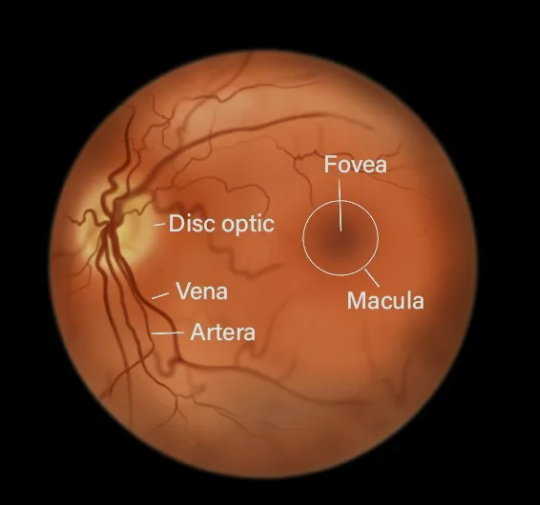
\includegraphics[width=0.7\columnwidth]{Figuri/Fund-de-Ochi.png}
\captionsetup{justification=centering}
\caption{Structura anatomică a fundului de ochi \cite{vitreum_fund_de_ochi}}
\label{fig:eye-fundus-anatomy}
\end{figure}

Principalele repere anatomice urmărite într-o imagine de fund de ochi sunt:

\begin{itemize}
  \item \textbf{Discul optic} -- regiune luminoasă din care pornesc vasele retiniene principale.
  \item \textbf{Macula} -- zonă responsabilă pentru vederea centrală, importantă în evaluarea edemului macular.
  \item \textbf{Foveea} -- centrul maculei, asociat cu acuitatea vizuală maximă.
  \item \textbf{Rețeaua vasculară} -- structură relevantă pentru identificarea hemoragiilor, microanevrismelor și modificărilor ischemice.
\end{itemize}

\bigskip

Vasele retiniene au o importanță deosebită în detectarea modificărilor patologice. În diabet,
afectarea microvasculară determină fragilizarea pereților capilari și modificări ale fluxului sanguin. Microanevrismele
apar ca mici dilatații ale capilarelor, fiind printre cele mai timpurii semne
vizibile ale retinopatiei diabetice. Hemoragiile sunt rezultatul ruperii sau scurgerii vaselor deteriorate,
iar exudatele apar prin depunerea de lipide și proteine în urma creșterii
permeabilității vasculare \cite{16_giancardo2012exudate}. În stadiile avansate, ischemia retiniană poate stimula formarea de
vase noi, fragile și anormale, fenomen numit neovascularizație \cite{18_wong2016diabetic}.
\bigskip

Din perspectiva prelucrării imaginilor, retina prezintă o combinație de structuri globale și
detalii locale fine. Structurile globale includ forma câmpului vizual, poziția discului optic
și distribuția vaselor principale, iar detaliile locale includ microanevrismele, punctele hemoragice,
exudatele mici sau modificările subtile de textură \cite{1_niemeijer2005automatic}, \cite{2_sopharak2009automatic}.
\bigskip

Un alt aspect relevant este diversitatea aspectului retinei: pigmentarea fundului de ochi,
diametrul vaselor și poziția discului optic pot varia între pacienți și între
achiziții. Modelele automate trebuie astfel să distingă între variații anatomice normale și
semne patologice reale, iar influența artefactelor de imagine este discutată separat în
secțiunea dedicată fotografiei fundus.

\section{Retinopatia diabetică -- definiție, stadii de evoluție și simptome}

\ \ \ \ Retinopatia diabetică este o complicație microvasculară a diabetului zaharat, caracterizată prin afectarea
progresivă a vaselor de sânge retiniene. Mecanismele patologice includ lezarea endoteliului vascular,
pierderea pericitelor, creșterea permeabilității capilare, ocluzii vasculare și ischemie retiniană. În timp,
aceste procese duc la apariția unor leziuni vizibile în imaginile fundului de
ochi. În fazele incipiente, pacientul poate să nu observe nicio modificare a
vederii, ceea ce face ca "screening-ul" periodic să fie esențial. În fazele
avansate, boala poate produce vedere încețoșată, pete în câmpul vizual, scăderea acuității
vizuale și, în cazuri severe, pierderea vederii \cite{18_wong2016diabetic}.
\bigskip

Clasificarea clinică a retinopatiei diabetice este de obicei organizată pe niveluri de
severitate. În lucrările de învățare automată, inclusiv în seturile de date publice
folosite frecvent, se utilizează adesea o scară cu cinci clase: \cite{3_gulshan2016development}, \cite{6_wang2021deep}, \cite{14_liu2022deepdrid} 
\begin{itemize}
  \item Clasa 0 -- fără retinopatie diabetică
  \item Clasa 1 -- retinopatie diabetică ușoară
  \item Clasa 2 -- retinopatie diabetică moderată
  \item Clasa 3 -- retinopatie diabetică severă 
  \item Clasa 4 -- retinopatie diabetică proliferativă
\end{itemize}

Această formulare este utilă pentru antrenarea modelelor de clasificare, deoarece transformă evaluarea clinică într-o problemă de
predicție multiclasă.
\bigskip

\begin{table}[H]
\centering
\caption{Interpretarea orientativă a claselor de severitate folosite în clasificarea retinopatiei diabetice}
\label{tab:stadii-dr}
\begin{tabular}{|c|p{4cm}|p{7cm}|}
\hline
\textbf{Clasa} & \textbf{Grad de severitate} & \textbf{Semne vizuale urmărite în imagine} \\
\hline
0 & Fără retinopatie diabetică & Nu sunt observate leziuni specifice; imaginea poate fi considerată normală din punct de vedere al retinopatiei diabetice. \\
\hline
1 & Retinopatie ușoară & Microanevrisme izolate, de obicei greu vizibile și ușor de confundat cu zgomot sau artefacte de achiziție. \\
\hline
2 & Retinopatie moderată & Număr mai mare de leziuni, cu posibile hemoragii, exudate dure și modificări vasculare vizibile. \\
\hline
3 & Retinopatie severă & Afectare vasculară extinsă, numeroase hemoragii și risc crescut de progresie către forma proliferativă. \\
\hline
4 & Retinopatie proliferativă & Neovascularizație și risc major de complicații severe, precum hemoragie vitroasă sau dezlipire de retină. \\
\hline
\end{tabular}
\end{table}

\begin{figure}[H]
\centering
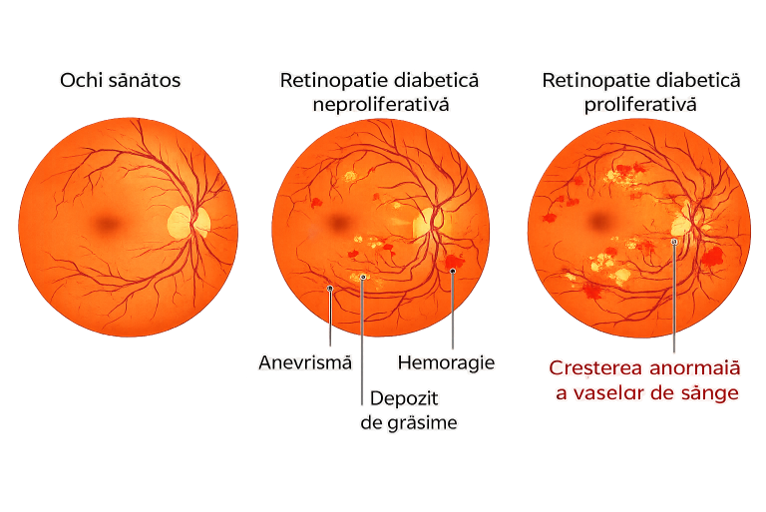
\includegraphics[width=0.95\columnwidth]{Figuri/neproli_vs_proli_eyes.png}
\captionsetup{justification=centering}
\caption{Reprezentare grafică a diferențelor vizuale între imagini cu, respectiv fără retinopatie \cite{vitreum_retinopatie_diabetica}}
\label{fig:proli-vs-nonproli}
\end{figure}
 
Clasele 0 și 1 sunt de obicei cele mai subtile din punct
de vedere vizual. Absența semnelor evidente într-o fotografie nu garantează absența completă
a riscului, deoarece detectabilitatea leziunilor depinde de calitatea imaginii și de câmpul
vizual acoperit. În același timp, retinopatia ușoară poate fi reprezentată doar de
câteva microanevrisme, motiv pentru care confuziile între clasele 0, 1 și 2
sunt frecvente în modelele automate \cite{3_gulshan2016development}, \cite{14_liu2022deepdrid}.
\bigskip

Clasele 3 și 4 sunt asociate cu afectare vasculară mai evidentă și
cu risc clinic mai ridicat. Imaginea devine, în general, mai evidentă din punct de vedere patologic,
iar modelele automate tind să obțină performanțe mai bune pentru aceste stadii
decât pentru cele incipiente. Totuși, identificarea corectă a claselor avansate este critică,
deoarece subestimarea severității poate întârzia intervenția medicală. Într-un sistem de screening, o
eroare de tip fals negativ pentru o formă proliferativă este mult mai
gravă decât o confuzie între două clase adiacente \cite{15_li2019diagnostic}.
\bigskip

În afara clasificării pe stadii, este importantă și natura leziunilor observabile. Cele
mai importante semne patologice sunt:

\begin{itemize}
  \item \textbf{Microanevrismele} -- printre primele semne ale bolii, vizibile ca puncte roșii foarte mici.
  \item \textbf{Hemoragiile} -- pot avea forme variate, de la punctiforme la pete mai extinse.
  \item \textbf{Exudatele dure} -- regiuni galben-albicioase, bine delimitate, asociate cu scurgeri lipidice.
  \item \textbf{Exudatele moi} -- pete vătămate care indică zone de ischemie în stratul fibrelor nervoase.
  \item \textbf{Neovascularizația} -- semn al trecerii către forma proliferativă.
\end{itemize}

Metodele automate pot aborda aceste semne fie prin clasificare globală a imaginii,
fie prin segmentarea leziunilor, fie prin combinații multi-task, în care modelul învață
simultan mai multe sarcini legate de severitate și localizare
\cite{1_niemeijer2005automatic}, \cite{2_sopharak2009automatic}, \cite{16_giancardo2012exudate}, \cite{18_wong2016diabetic}, \cite{6_wang2021deep}, \cite{7_huang2022rtnet}.

\section{Imagistica de fund de ochi ("fundus photography")}

\ \ \ \ Fotografia de fund de ochi reprezintă una dintre cele mai utilizate metode
de examinare imagistică a retinei. Aceasta permite captarea unei imagini color a
suprafeței retiniene, incluzând discul optic, vasele sanguine, macula și eventualele leziuni patologice.
Spre deosebire de metode mai complexe, precum angiografia cu fluoresceină sau tomografia
în coerență optică, fotografia fundus este relativ rapidă, neinvazivă și potrivită pentru
programe de "screening" la scară largă \cite{3_gulshan2016development}. Din acest motiv, majoritatea seturilor
de date utilizate în cercetarea privind detecția automată a retinopatiei diabetice se
bazează pe astfel de imagini \cite{9_chetoui2020explainable}, \cite{14_liu2022deepdrid}.
\bigskip

În mod obișnuit, o imagine fundus este obținută cu o cameră specializată
care iluminează retina și captează lumina reflectată prin pupilă. Achiziția poate fi
realizată cu sau fără dilatarea pupilei, iar câmpul vizual poate varia în
funcție de echipament. Imaginile pot avea rezoluții diferite, niveluri diferite de contrast
și grade variabile de claritate. În plus, pot apărea artefacte precum reflexii
luminoase, umbre, zone întunecate, margini circulare, praf pe lentilă sau defocalizare. Toate
aceste elemente influențează atât evaluarea umană, cât și performanța algoritmilor de clasificare
\cite{14_liu2022deepdrid}, \cite{8_zhang2022multi}.
\bigskip

Pentru analiza automată, imaginea fundus prezintă mai multe provocări. Prima este variația
de iluminare. Unele imagini sunt supraexpuse, iar leziunile luminoase pot fi greu
de distins de fundal. Altele sunt subexpuse, iar leziunile roșii sau vasele
fine pot deveni slab vizibile. A doua provocare este variația cromatică: tonul
general al retinei diferă între pacienți și între camere. A treia provocare
este rezoluția foarte mare a imaginilor originale. Leziunile mici pot ocupa doar
câțiva pixeli, iar redimensionarea agresivă poate elimina informație relevantă. În același timp,
procesarea directă a imaginilor la rezoluție completă poate fi costisitoare computațional
\cite{3_gulshan2016development}, \cite{11_shakibania2024dual}.
\bigskip

Cele mai frecvente dificultăți întâlnite în imaginile de fund de ochi sunt:

\begin{itemize}
  \item variații de iluminare și contrast între imagini;
  \item diferențe cromatice între pacienți și între camere de achiziție;
  \item rezoluții diferite și dimensiuni mari ale imaginilor originale;
  \item artefacte precum reflexii, blur, margini întunecate sau câmp vizual incomplet;
  \item dimensiunea foarte mică a unor leziuni, în special a microanevrismelor.
\end{itemize}

\bigskip

Preprocesarea imaginilor are rolul de a reduce aceste variații și de a
oferi modelului date mai consistente. Etapele frecvente includ decuparea marginilor negre, redimensionarea
la o dimensiune standard, normalizarea valorilor pixelilor, corectarea iluminării și aplicarea unor
transformări de augmentare. În unele abordări, se utilizează metode pentru evidențierea vaselor
sau pentru îmbunătățirea contrastului local. În altele, modelul primește imaginea aproape brută,
iar rețeaua neuronală învață singură trăsăturile relevante. Alegerea depinde de dimensiunea setului
de date, de arhitectura folosită și de obiectivul experimentului
\cite{2_sopharak2009automatic}, \cite{13_staal2004ridge}, \cite{9_chetoui2020explainable}.
\bigskip

Într-un flux tipic de lucru, preprocesarea poate include:

\begin{itemize}
  \item decuparea zonelor negre din jurul câmpului circular al imaginii;
  \item redimensionarea imaginilor la dimensiunea cerută de model;
  \item normalizarea intensităților pixelilor;
  \item corectarea parțială a iluminării neuniforme;
  \item augmentări precum rotații, flip-uri, modificări de luminozitate sau contrast.
\end{itemize}

\bigskip

Din punct de vedere practic, preprocesarea trebuie să păstreze leziunile fine, nu
doar să uniformizeze aspectul general al imaginii. O redimensionare prea agresivă poate
elimina microanevrismele, iar o corecție de contrast nepotrivită poate accentua artefactele. De
aceea, etapele de preprocesare sunt alese în funcție de modelul folosit și
de rezoluția minimă la care semnele patologice rămân vizibile.
\bigskip

Aceste observații sunt importante pentru proiectarea fluxului experimental: imaginile trebuie aduse
la o formă comparabilă fără a elimina informația patologică fină. Diferența dintre
abordările bazate pe trăsături proiectate manual și cele bazate pe învățare profundă este
discutată în secțiunea următoare
\cite{1_niemeijer2005automatic}, \cite{2_sopharak2009automatic}, \cite{4_pratt2016convolutional}.
\bigskip

Un element important în folosirea imaginilor fundus pentru clasificare este raportul dintre
informația globală și cea locală. O imagine poate conține semne patologice mici,
dar decizia finală depinde și de distribuția acestora în câmpul retinian. Un
model care analizează doar fragmente locale poate detecta leziuni, dar poate pierde
contextul global. Un model care analizează imaginea întreagă poate învăța distribuția generală,
dar poate rata detalii fine după redimensionare. Din acest motiv, literatura recentă
explorează arhitecturi care combină informații la mai multe scări, ramuri multiple sau
mecanisme de atenție \cite{11_shakibania2024dual}, \cite{7_huang2022rtnet}.

\section{Diagnosticul clinic -- procesul actual și limitările sale}

\ \ \ \ Diagnosticul clinic al retinopatiei diabetice se bazează pe evaluarea imaginilor retiniene de
către medici oftalmologi sau specialiști instruiți în screening. În cadrul unui flux
standard, pacientului i se realizează una sau mai multe fotografii ale fundului
de ochi, iar imaginile sunt analizate pentru identificarea leziunilor specifice. În funcție
de severitate, pacientul poate fi încadrat într-o categorie de risc și poate
primi recomandări pentru monitorizare, investigații suplimentare sau tratament. În programele de screening,
scopul principal este identificarea pacienților care necesită evaluare medicală mai rapidă, înainte
de apariția pierderii ireversibile de vedere \cite{3_gulshan2016development}, \cite{15_li2019diagnostic}.
\bigskip

Procesul clinic are însă mai multe limitări \cite{3_gulshan2016development}, \cite{14_liu2022deepdrid}:

\begin{itemize}
  \item \textbf{Disponibilitatea specialiștilor:} Pe măsură ce numărul pacienților cu diabet crește, volumul imaginilor
    care trebuie evaluate devine tot mai mare.
  \item \textbf{Variabilitatea opiniei între observatori:} Doi specialiști pot evalua diferit aceeași imagine, mai ales în
    cazurile de graniță dintre clase.
  \item \textbf{Variabilitatea intra-observator:} Același specialist poate avea discrepanțe în decizie în funcție de
    oboseală, experiență sau calitatea imaginii.
  \item \textbf{Calitatea imaginilor:} Imaginile slab focalizate, întunecate sau parțial acoperite de artefacte sunt greu de interpretat.
\end{itemize}
\bigskip

În practică, problema calității imaginii rămâne deosebit de importantă. În unele cazuri,
imaginea trebuie repetată, ceea ce crește timpul și costul examinării. În alte
cazuri, imaginea poate fi evaluată cu incertitudine, ceea ce afectează consistența diagnosticului.
Din acest motiv, unele sisteme moderne includ nu doar clasificarea retinopatiei, ci
și estimarea calității imaginii, astfel încât imaginile neinterpretabile să fie semnalate separat
\cite{14_liu2022deepdrid}.
\bigskip

Sistemele automate bazate pe inteligență artificială nu înlocuiesc medicul, dar pot funcționa
ca instrumente de suport. Într-un scenariu de "screening", un algoritm poate analiza
rapid un număr mare de imagini și poate prioritiza cazurile suspecte. De
asemenea, poate oferi o a doua opinie sau poate reduce timpul necesar
pentru trierea imaginilor fără semne evidente. Studiile moderne au demonstrat că modelele
de învățare profundă pot atinge performanțe ridicate în detectarea retinopatiei diabetice pe
imagini fundus \cite{3_gulshan2016development}, \cite{15_li2019diagnostic}. Totuși, integrarea clinică necesită validare riguroasă, interpretabilitate, robustețe
la imagini din surse diferite și control al erorilor critice.
\bigskip

O dificultate specifică diagnosticului automat este faptul că nu toate erorile au
aceeași importanță. În clasificarea multiclasă, o predicție greșită cu o clasă adiacentă
poate fi tolerabilă în anumite contexte, dar o predicție care subestimează severitatea
bolii poate întârzia tratamentul. De exemplu, clasificarea unei imagini severe ca fiind
fără retinopatie este o eroare mult mai periculoasă decât clasificarea unei imagini
moderate ca ușoare. Din acest motiv, evaluarea unui model nu trebuie să
se bazeze exclusiv pe acuratețe globală, ci pe un set mai larg
de metrici \cite{15_li2019diagnostic}, \cite{14_liu2022deepdrid}:

\begin{itemize}
  \item \textbf{Sensibilitate} (\textit{Sensitivity / Recall}) -- exprimă proporția cazurilor patologice detectate corect de model.
   În context medical, această metrică este importantă deoarece un scor scăzut indică existența unor cazuri de boală ratate 
   (\textit{false negatives}), ceea ce poate afecta diagnosticul precoce.

  \item \textbf{Specificitate} (\textit{Specificity}) -- exprimă proporția cazurilor sănătoase identificate corect.
   O specificitate ridicată indică faptul că modelul produce puține alarme false și nu clasifică eronat pacienții sănătoși ca fiind bolnavi.

  \item \textbf{Scorul AUC} (\textit{Area Under the ROC Curve}) -- evaluează capacitatea modelului de a separa clasele 
  pentru diferite praguri de decizie. Un scor AUC apropiat de 1 indică o separare foarte bună, iar un scor apropiat de 
  0.5 sugerează o performanță slabă, comparabilă cu alegerea aleatoare.

  \item \textbf{Matricea de confuzie} -- oferă o reprezentare detaliată a relației dintre clasele reale și cele prezise. 
  Aceasta permite identificarea tipurilor de erori produse de model și evidențierea claselor care sunt confundate frecvent.

  \item \textbf{Performanța pe fiecare clasă} -- este necesară mai ales în cazul seturilor de date dezechilibrate.
   Prin raportarea valorilor de \textit{precision}, \textit{recall} și \textit{F1-score} pentru fiecare clasă, se poate
    evalua dacă modelul funcționează bine doar pentru clasele majoritare sau și pentru cele rare, dar importante clinic.
\end{itemize}

\section{Învățarea automată și învățarea profundă în analiza imaginilor medicale}

\ \ \ \ Învățarea automată este un domeniu al inteligenței artificiale care urmărește dezvoltarea unor
algoritmi capabili să învețe modele din date. În loc ca regulile să
fie definite explicit de programator, sistemul ajustează parametri interni pe baza unor
exemple. În cazul clasificării imaginilor medicale, exemplele sunt imagini asociate cu etichete
clinice, iar obiectivul modelului este să învețe o funcție care primește o
imagine și produce o predicție. Pentru retinopatia diabetică, această predicție poate fi
binară, de tipul retinopatie prezentă/absentă, sau multiclasă, corespunzătoare severității bolii \cite{3_gulshan2016development}, \cite{15_li2019diagnostic}.
\bigskip

Metodele clasice de învățare automată necesitau de obicei o etapă separată de
extragere a trăsăturilor. În imaginile retiniene, aceste trăsături puteau include culoarea, textura,
forma leziunilor, grosimea vaselor sau distribuția spațială a exudatelor. După extragerea trăsăturilor,
un clasificator precum SVM, k-NN sau Random Forest putea fi antrenat pentru
a lua decizia finală. Avantajul acestor metode este interpretabilitatea relativ mai mare
a unor trăsături proiectate manual. Dezavantajul este dependența puternică de calitatea acestor
trăsături și dificultatea de a acoperi toată aria și diversitatea imaginilor reale
\cite{1_niemeijer2005automatic}, \cite{2_sopharak2009automatic}, \cite{13_staal2004ridge}.
\bigskip

Într-o abordare clasică, "pipeline"-ul era de obicei împărțit în etape distincte:

\begin{itemize}
  \item preprocesarea imaginii și corectarea iluminării;
  \item extragerea manuală a trăsăturilor relevante;
  \item selectarea sau reducerea dimensionalității trăsăturilor;
  \item antrenarea unui clasificator clasic;
  \item validarea rezultatului pe imagini nefolosite la antrenare.
\end{itemize}

\bigskip

Învățarea profundă schimbă această paradigmă prin folosirea unor rețele neuronale cu multe
straturi, capabile să învețe reprezentări ierarhice \cite{19_lecun2015deep}. Într-o rețea convoluțională, primele straturi
învață filtre simple, precum muchii, contraste locale sau texturi. Straturile intermediare combină
aceste filtre în forme mai complexe, iar straturile profunde pot reprezenta structuri
relevante pentru sarcina finală. Această ierarhie este potrivită pentru imagini medicale, deoarece
semnele patologice apar la scări diferite și în contexte anatomice variate
\cite{19_lecun2015deep}, \cite{4_pratt2016convolutional}.
\bigskip

În procesul de antrenare supervizată, modelul primește perechi imagine-etichetă și produce o
predicție. Diferența dintre predicție și eticheta reală este măsurată printr-o funcție de
pierdere, iar parametrii rețelei sunt actualizați prin algoritmi de optimizare, de obicei
pe baza propagării inverse a gradientului. Pentru clasificarea multiclasă, se pot utiliza
mai multe tipuri de funcții de pierdere, fiecare abordând problema dintr-o perspectivă diferită:

\begin{itemize}
  \item \textbf{Cross-Entropy (CE)} -- este funcția standard pentru problemele de clasificare multiclasă. 
  Aceasta măsoară divergența dintre distribuția de probabilitate prezisă de model și distribuția reală a etichetelor. 
  Funcționează optim atunci când setul de date este echilibrat, dar poate favoriza clasele majoritare în scenarii dezechilibrate.
  \item \textbf{Weighted Cross-Entropy (WCE)} -- reprezintă o extensie a funcției standard, introdusă pentru a combate dezechilibrul 
  claselor. Prin asocierea unei ponderi mai mari erorilor provenite din clasele rare (minoritare), modelul este penalizat 
  mai sever dacă greșește în aceste cazuri, asigurând o învățare echitabilă și performanțe superioare pentru clasele critice.
  \item \textbf{Focal Loss} -- este o funcție avansată concepută special pentru a rezolva problema dezechilibrului
  extrem și a exemplelor greu de separat. Aceasta modifică ecuația standard prin introducerea unui factor de modulare care reduce semnificativ contribuția exemplelor clasificate ușor și forțează modelul să se concentreze prioritar pe exemplele dificile (\textit{hard examples}) \cite{20_lin2017focal}.
\end{itemize}

\bigskip

Dezechilibrul claselor este o problemă frecventă în retinopatia diabetică. În multe seturi
de date, clasa fără retinopatie este mult mai numeroasă decât clasele severe.
Dacă modelul este antrenat fără corecții, acesta poate obține acuratețe bună prin
favorizarea clasei dominante, dar poate avea sensibilitate slabă pentru clasele rare. Din
acest motiv, evaluarea trebuie să urmărească performanța pe fiecare clasă, nu doar
media globală. Tehnicile de reechilibrare includ ponderarea funcției de pierdere, eșantionarea echilibrată,
augmentare mai puternică a claselor minoritare sau folosirea unor metrici robuste la dezechilibru
\cite{20_lin2017focal}, \cite{14_liu2022deepdrid}.
\bigskip

\begin{figure}[H]
\centering
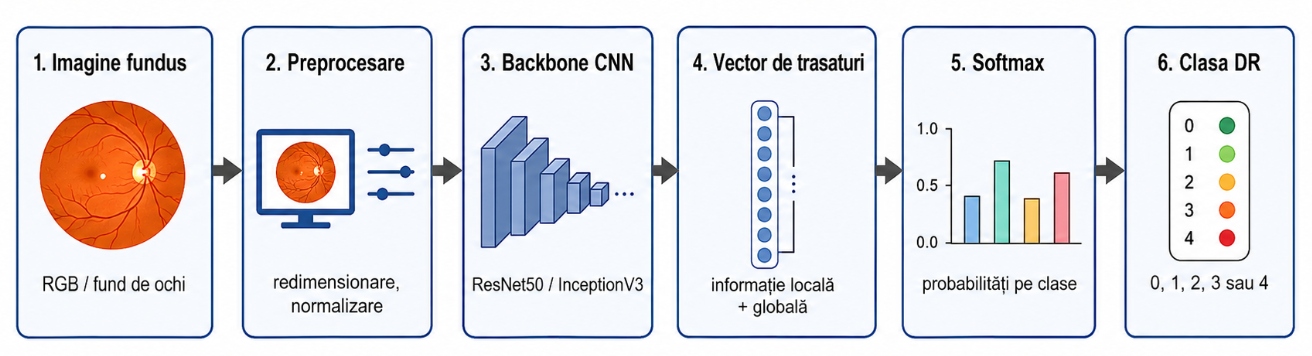
\includegraphics[width=0.95\columnwidth]{Figuri/schema_flux_cnn.png}
\captionsetup{justification=centering}
\caption{Flux conceptual pentru clasificarea imaginilor de fund de ochi cu o rețea neuronală convoluțională}
\label{fig:schema-flux-cnn}
\end{figure}

În analiza imaginilor medicale, o altă provocare este dimensiunea limitată a datelor
adnotate. Obținerea etichetelor clinice necesită timp și expertiză, iar datele pot fi
afectate de restricții etice și de confidențialitate. Una dintre soluțiile folosite frecvent
pentru această problemă este transfer learning-ul, prezentat separat la finalul capitolului
\cite{10_jabbar2022transfer}.

\section{Rețele neuronale convoluționale}

\ \ \ \ Rețelele neuronale convoluționale, cunoscute sub abrevierea CNN, reprezintă una dintre cele mai
importante arhitecturi pentru analiza imaginilor. Ele sunt concepute pentru a exploata structura
spațială a datelor vizuale. Spre deosebire de o rețea complet conectată, care
ar trata fiecare pixel independent de poziția sa, o rețea convoluțională aplică
filtre locale pe imagine și păstrează relațiile spațiale dintre pixeli. Această proprietate
este esențială pentru imagini retiniene, deoarece semnele patologice sunt definite de configurații
locale de culoare, formă și textură \cite{4_pratt2016convolutional}, \cite{9_chetoui2020explainable}.
\bigskip

Operația de convoluție constă în deplasarea unui filtru peste imagine și calcularea
unui răspuns local. Fiecare filtru învață să detecteze un anumit tipar vizual.
În primele straturi, filtrele pot detecta margini, pete sau contraste. În straturile
mai profunde, combinațiile de filtre pot detecta structuri mai complexe, precum vase,
exudate sau zone hemoragice. Parametrii filtrelor sunt învățați automat în timpul antrenării,
ceea ce elimină necesitatea proiectării manuale a descriptorilor vizuali
\cite{19_lecun2015deep}, \cite{4_pratt2016convolutional}.
\bigskip

Pe lângă straturile convoluționale, CNN-urile includ mai multe componente recurente, așa cum se poate observa 
și în figura \ref{fig:cnn}:

\begin{itemize}
  \item \textbf{funcții de activare}, care introduc neliniaritate și permit modelului să aproximeze relații complexe;
  \item \textbf{operații de pooling}, care reduc dimensiunea spațială a hărților de trăsături;
  \item \textbf{straturi de normalizare}, care pot stabiliza antrenarea și accelera convergența;
  \item \textbf{straturi complet conectate sau globale}, care transformă trăsăturile extrase într-o predicție finală;
  \item \textbf{strat softmax}, folosit frecvent pentru a obține probabilități pe clase în clasificarea multiclasă.
\end{itemize}
\bigskip

\begin{figure}[H]
\centering
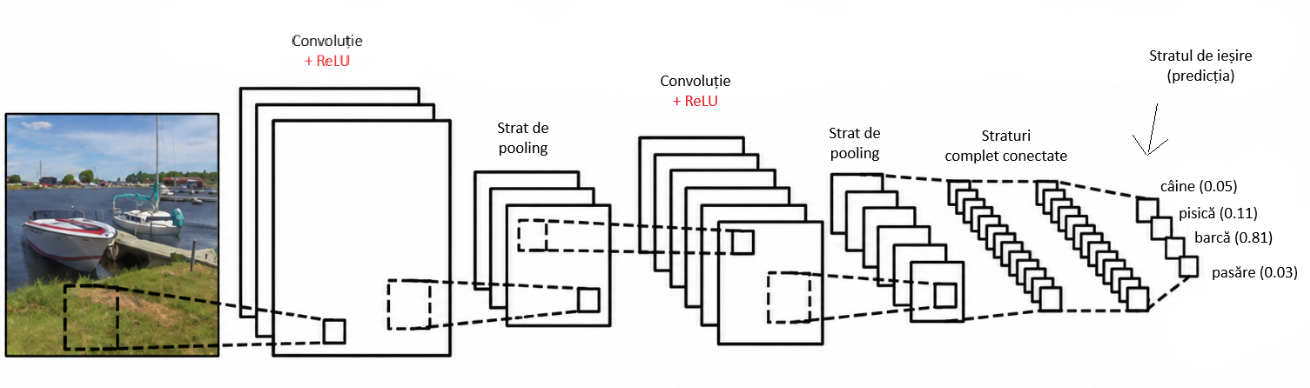
\includegraphics[width=0.95\columnwidth]{Figuri/cnn.png}
\captionsetup{justification=centering}
\caption{Schema generală a unei rețele neuronale convoluționale \cite{master_taid_cnn}}
\label{fig:cnn}
\end{figure}

Arhitecturile CNN moderne diferă prin adâncime, tipul blocurilor folosite și modul în
care gestionează propagarea informației. Dintre acestea, câteva arhitecturi s-au remarcat în mod special în analiza imaginilor medicale:

\begin{itemize}
  \item \textbf{ResNet (Residual Networks)} -- introduce conexiuni reziduale (``skip connections''), care permit transmiterea directă 
  a informației peste unul sau mai multe straturi \cite{21_he2016deep}. Această inovație atenuează problema dispariției gradientului 
  și previne degradarea 
  \newline performanței în rețelele foarte adânci, facilitând învățarea unor reprezentări vizuale complexe.
  
  \begin{figure}[H]
  \centering
  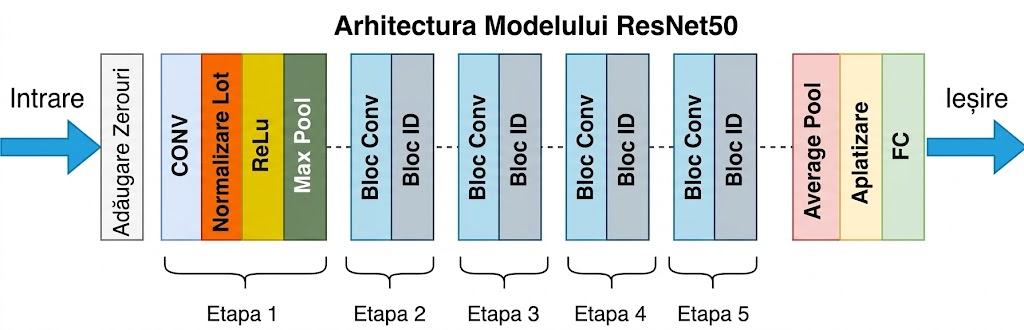
\includegraphics[width=0.8\columnwidth]{Figuri/resnet50.png}
  \captionsetup{justification=centering}
  \caption{Schema unei arhitecturi ResNet50 \cite{researchgate_resnet50_diagram}}
  \label{fig:resnet50}
  \end{figure}
  
  \item \textbf{Inception} -- utilizează module care aplică simultan filtre convoluționale de dimensiuni diferite 
  (ex. 1$\times$1, 3$\times$3, 5$\times$5) pe aceeași intrare, capturând astfel informații la scări spațiale multiple 
  \cite{22_szegedy2016rethinking}. Acest mecanism este crucial în retinopatia diabetică, unde patologia variază de la leziuni minuscule
  (microanevrisme punctiforme) la zone masive (exudate extinse sau hemoragii).
  
  \begin{figure}[H]
  \centering
  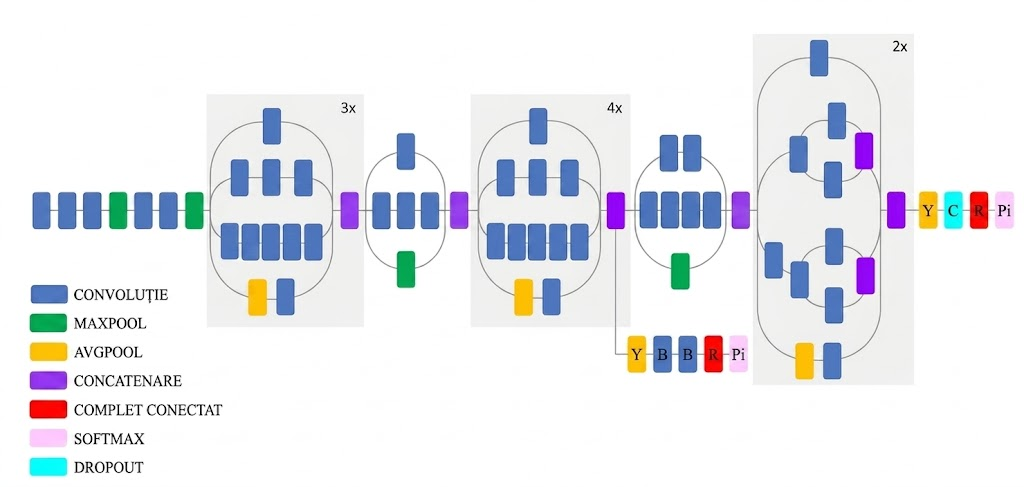
\includegraphics[width=0.8\columnwidth]{Figuri/inception-v3.png}
  \captionsetup{justification=centering}
  \caption{Schema unei arhitecturi Inception-v3 \cite{researchgate_inceptionv3_diagram}}
  \label{fig:inception-v3}
  \end{figure}

  \item \textbf{EfficientNet-B3} -- face parte din familia EfficientNet, arhitecturi care folosesc o strategie de 
  scalare compusă (\textit{compound scaling}) pentru a crește simultan adâncimea, lățimea și rezoluția rețelei într-un
  mod echilibrat. Varianta B3 oferă un compromis între acuratețe și cost computațional, fiind potrivită pentru 
  imagini medicale unde detaliile fine trebuie păstrate fără a crește excesiv complexitatea modelului. 
  În contextul retinopatiei diabetice, această arhitectură poate ajuta la identificarea leziunilor subtile, 
  precum microanevrismele sau exudatele mici, menținând în același timp capacitatea de a surprinde contextul global 
  al imaginii fundus \cite{tan2019efficientnet}.

  \begin{figure}[H]
  \centering
  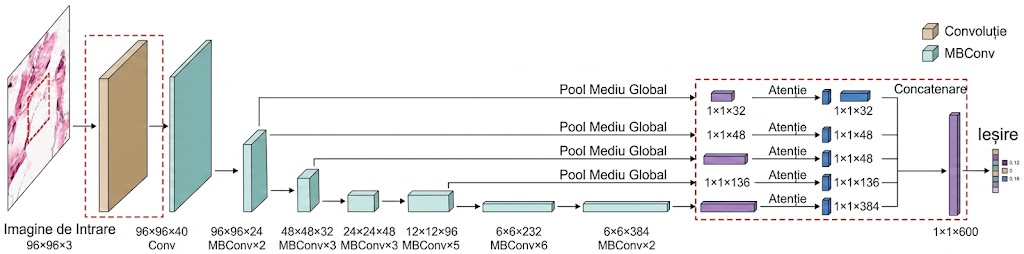
\includegraphics[width=0.8\columnwidth]{Figuri/boosted-efficientnet-b3.png}
  \captionsetup{justification=centering}
  \caption{Schema unei arhitecturi EfficientNet-B3 \cite{wang2021boosted_efficientnet}}
  \label{fig:efficientnet-b3}
  \end{figure}  

  \item \textbf{Inception-ResNet} -- reprezintă o arhitectură hibridă care combină eficiența de procesare multi-scală a modulelor Inception
  cu propagarea robustă a gradientului oferită de conexiunile reziduale. Această fuziune crește viteza de convergență și oferă o 
  capacitate superioară de generalizare, aspect esențial pentru imaginile cu patologii retiniene complexe
  \cite{10_jabbar2022transfer}, \cite{11_shakibania2024dual}.

  \begin{figure}[H]
  \centering
  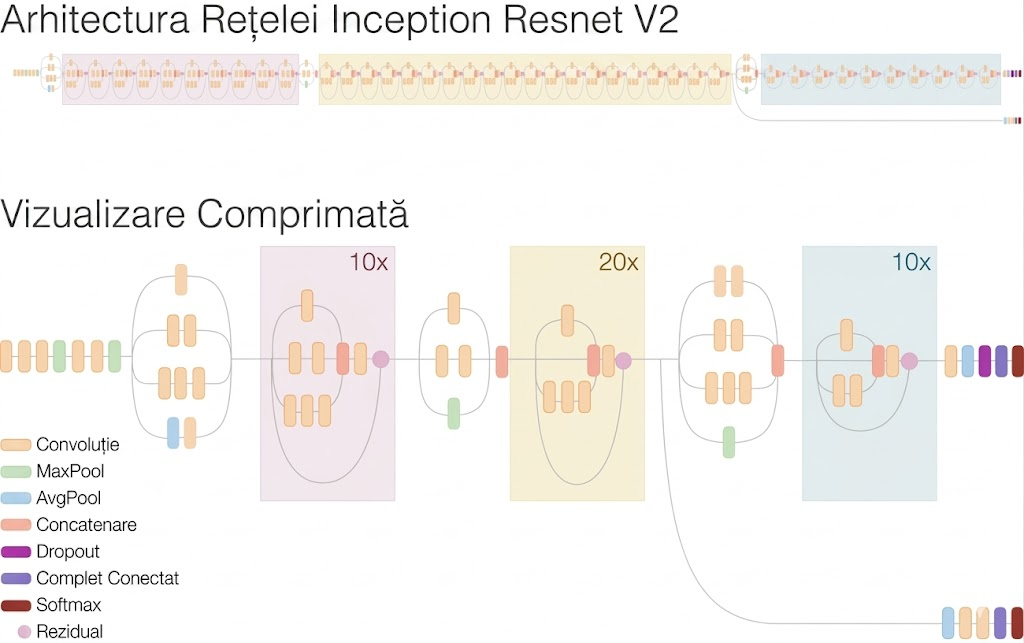
\includegraphics[width=0.8\columnwidth]{Figuri/incres-v2.png}
  \captionsetup{justification=centering}
  \caption{Schema unei arhitecturi Inception-ResNet-v2 \cite{researchgate_inception_resnet_v2_diagram}}
  \label{fig:incres-v2}
  \end{figure}

\end{itemize}
\bigskip

În retinopatia diabetică, CNN-urile pot fi folosite în mai multe moduri:

\begin{itemize}
  \item \textbf{clasificare globală}, în care modelul primește fotografia fundus și produce gradul de severitate;
  \item \textbf{detecție de leziuni}, în care modelul indică prezența unor semne patologice;
  \item \textbf{segmentare semantică}, în care modelul identifică regiunile afectate la nivel de pixel;
  \item \textbf{modele hibride sau multi-task}, care învață simultan clasificarea, localizarea și interpretarea leziunilor.
\end{itemize}

Segmentarea poate oferi informație mai detaliată și poate susține interpretabilitatea, dar necesită
etichete "pixel-level", mai greu de obținut. Metodele hibride combină ramuri globale și
locale pentru a integra contextul cu detaliile patologice
\cite{6_wang2021deep}, \cite{7_huang2022rtnet}, \cite{11_shakibania2024dual}.
\bigskip

Un aspect important al CNN-urilor este interpretabilitatea. Deși performanța lor poate fi
ridicată, modelele profunde sunt adesea percepute ca sisteme de tip ``cutie neagră''.
În medicină, această problemă este critică, deoarece deciziile trebuie să fie verificabile
și explicabile. Tehnici precum hărțile de activare a claselor pot evidenția regiunile
care au influențat predicția, oferind medicului o indicație vizuală asupra motivului pentru
care modelul a ales o anumită clasă. Astfel de metode nu garantează
corectitudinea deciziei, dar pot crește transparența și pot ajuta la detectarea cazurilor
în care modelul se bazează pe artefacte sau regiuni irelevante \cite{9_chetoui2020explainable}.

\section{Transfer learning și modele pre-antrenate}

\ \ \ \ Transfer learning-ul este o tehnică prin care cunoștințele învățate într-o sarcină sunt
reutilizate pentru o altă sarcină. În contextul imaginilor medicale, această tehnică este
foarte importantă deoarece seturile de date adnotate sunt mai greu de obținut
decât în domeniile generale ale vederii computerizate. Un model pre-antrenat pe milioane
de imagini poate învăța filtre generale pentru muchii, texturi, forme și compoziții
vizuale. Chiar dacă imaginile naturale diferă de imaginile retiniene, primele straturi ale
rețelei pot rămâne utile, iar straturile finale pot fi adaptate la clasificarea
medicală \cite{10_jabbar2022transfer}, \cite{19_lecun2015deep}.
\bigskip

Există mai multe moduri de utilizare a transfer learning-ului:

\begin{itemize}
  \item \textbf{Extractor de trăsături fix.} Straturile convoluționale sunt păstrate fixe, iar doar clasificatorul
    final este antrenat pe datele medicale.
  \item \textbf{Fine-tuning parțial.} Se ajustează doar ultimele blocuri ale rețelei, pentru a adapta
    reprezentările la imaginile retiniene.
  \item \textbf{Fine-tuning complet.} Toți parametrii modelului sunt actualizați, variantă utilă când există suficiente
    date și regularizare adecvată.
\end{itemize}

Fine-tuning-ul poate oferi performanțe mai bune, dar necesită atenție la rata de
învățare, dimensiunea setului de date, regularizare și optimizatorul folosit, Adam fiind una
dintre alegerile frecvente în antrenarea rețelelor profunde \cite{10_jabbar2022transfer}, \cite{23_kingma2014adam}.
\bigskip

În aplicații de retinopatie diabetică, arhitecturile pre-antrenate pot fi adaptate prin
înlocuirea ultimului strat cu un clasificator pentru cele cinci clase de severitate și
prin continuarea antrenării pe imaginile fundus disponibile \cite{4_pratt2016convolutional}, \cite{10_jabbar2022transfer}. Detaliile arhitecturilor utilizate experimental sunt
prezentate ulterior în metodologia propusă.
\bigskip

Transfer learning-ul nu elimină însă toate problemele. Dacă datele de antrenare sunt
dezechilibrate sau conțin artefacte sistematice, modelul poate învăța corelații nedorite. De exemplu,
dacă imaginile severe provin predominant de la o anumită cameră sau au
o anumită rezoluție, modelul poate asocia caracteristicile tehnice cu boala. Această problemă
este cunoscută ca bias de domeniu și afectează capacitatea de generalizare. Din
acest motiv, este importantă evaluarea pe seturi de validare și testare reprezentative,
precum și analiza erorilor prin matrice de confuzie și curbe ROC \cite{8_zhang2022multi}, \cite{14_liu2022deepdrid}.
\bigskip

În această lucrare, fundamentele prezentate în capitolul curent susțin partea experimentală ulterioară.
Retinopatia diabetică este o problemă medicală cu impact ridicat, imaginile de fund
de ochi oferă suportul vizual pentru screening automat, iar rețelele convoluționale permit
învățarea directă a trăsăturilor relevante. Transfer learning-ul facilitează adaptarea arhitecturilor moderne la
date medicale, iar metricile de evaluare permit compararea configurațiilor de antrenare. Împreună,
aceste elemente definesc cadrul teoretic necesar pentru metodologia propusă și pentru interpretarea
rezultatelor experimentale.


\chapter{Stadiul actual al cercetării}

\section{Analiza seturilor de date disponibile}

\ \ \ \ Performanța și capacitatea de generalizare a modelelor de învățare profundă sunt intrinsec
dependente de calitatea, volumul și diversitatea datelor utilizate în procesul de antrenare. În contextul
oftalmologiei computaționale, disponibilitatea bazelor de date publice a permis tranziția de la metodele
clasice de procesare a imaginii la arhitecturi neuronale complexe, oferind un teren comun pentru
evaluarea obiectivă a algoritmilor.

\begin{itemize}
  \item \textbf{Seturi de referință pentru clasificarea globală (“Grading”)}
  
      \begin{itemize}
          \item \textbf{EyePACS} (Kaggle Diabetic Retinopathy Detection) \cite{3_gulshan2016development}, \cite{9_chetoui2020explainable} rămâne cea mai 
                vastă resursă publică disponibilă, conținând aproximativ 88.702 de imagini. Importanța sa constă în caracterul eterogen al
                imaginilor (variații de expunere, focalizare, artefacte), fiind critic pentru antrenarea unor
                rețele backbone robuste capabile să gestioneze fenomenul de “domain shift” \cite{8_zhang2022multi} și să generalizeze pe
                imagini de calitate slabă

          \item \textbf{APTOS 2019} Blindness Detection \cite{9_chetoui2020explainable} reprezintă standardul modern de calitate. Colectat de Aravind Eye
                Hospital, acest set de 3.662 de imagini este utilizat frecvent în literatura recentă pentru “fine-tuning”,
                oferind o vizibilitate superioară a detaliilor retiniene comparativ cu seturile mai vechi

          \item \textbf{MESSIDOR-2} \cite{9_chetoui2020explainable} este considerat în prezent „Benchmark-ul de Aur” pentru testarea algoritmilor.
                Extinzând setul original Messidor la 1.748 de imagini, acesta se distinge prin consistența diagnostică și
                este utilizat ca domeniu țintă (Target Domain) în studiile de adaptare \cite{8_zhang2022multi} și pentru validarea sistemelor
                explicabile (XAI) \cite{9_chetoui2020explainable}, oferind o metrică fidelă a performanței reale pe date curate.

          \item \textbf{DeepDRiD} \cite{14_liu2022deepdrid} aduce o inovație necesară prin structurarea
                celor 2.000 de imagini în perechi binoculare și includerea notelor de calitate, simulând fluxul de triaj
                clinic.

          \item \textbf{UoA-DR} \cite{9_chetoui2020explainable} este o resursă istorică (~200 imagini), utilizată
                complementar în studiile comparative pentru a asigura diversitatea demografică a validării.
      \end{itemize}

  \item \textbf{Seturi specializate pentru segmentarea leziunilor și analiza detaliată}

      \begin{itemize}
        \item \textbf{IDRiD} \cite{9_chetoui2020explainable} este setul critic pentru sarcinile de segmentare
              semantică fină \cite{7_huang2022rtnet}. Pentru 81 dintre imagini, experții au trasat manual măști
              binare la nivel de pixel,
              făcându-l indispensabil pentru antrenarea arhitecturilor complexe de tip Transformer și pentru validarea
              localizării leziunilor în sistemele end-to-end \cite{9_chetoui2020explainable}.

        \item \textbf{DDR} \cite{15_li2019diagnostic} a revoluționat segmentarea pe scară largă, oferind 13.673 de
              imagini. Este esențial pentru antrenarea rețelelor adânci de segmentare (precum RTNet) fără a risca
              “overfitting-ul”, oferind adnotări “pixel-wise” pentru leziuni multiple \cite{7_huang2022rtnet}.

        \item \textbf{E-Ophtha} \cite{9_chetoui2020explainable} este o bază de date vitală pentru reducerea alarmelor false
          în metodele de detecție a
              exudatelor \cite{2_sopharak2009automatic}. Valoarea sa unică constă în includerea imaginilor cu patologii non-diabetice care pot fi
              confundate cu DR

        \item \textbf{DiaRetDB1} \cite{9_chetoui2020explainable} este standardul istoric pentru calibrarea sensibilității la leziuni roșii (microanevrisme) în
              lucrările de detecție automată \cite{1_niemeijer2005automatic}. Complementar, HEI-MED \cite{16_giancardo2012exudate} oferă 169 de imagini focalizate exclusiv
              pe segmentarea zonelor de Edem Macular Diabetic.

        \begin{figure}[h]
        \centering
        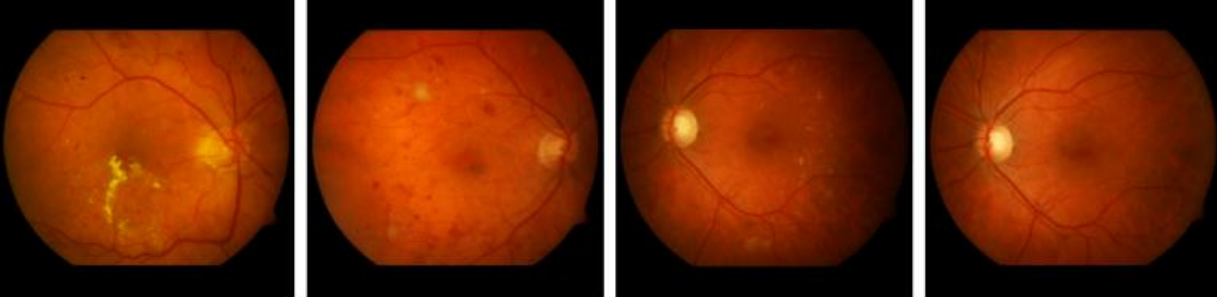
\includegraphics[width=1\columnwidth]{Figuri/Fig1_Eye-fundus-examples.png}
        \captionsetup{justification=centering}
        \caption{Exemple de imagini ale fundului de ochi în seturile de date DIARETDB0 și DIARETDB1 \cite{9_chetoui2020explainable}}
        \label{fig: Examples-fundus-eyes}
        \end{figure}

      \end{itemize}

  \item \textbf{Seturi standard pentru preprocesarea vasculară}
  
        \begin{itemize}
          \item \textbf{DRIVE} \cite{13_staal2004ridge} și \textbf{STARE} \cite{9_chetoui2020explainable} sunt pilonii etapei de preprocesare.
                Deși conțin un număr redus de imagini, ele sunt utilizate obligatoriu pentru validarea algoritmilor de
                segmentare a vaselor de sânge, cum ar fi arhitecturile U-Net modificate \cite{12_sambyal2020modified} sau metodele clasice de
                extragere a trăsăturilor \cite{1_niemeijer2005automatic}.

                Tabelul de mai jos sintetizează caracteristicile tehnice esențiale ale seturilor de date analizate,
                evidențiind diferențele de volum, rezoluție și tipul de adnotare disponibil, elemente care dictează
                utilizarea lor în diversele etape ale proiectului.

            \begin{table}[H]
            \centering
            \small
            \caption{Tabel comparativ între seturile de date disponibile}
            \label{tab:datasets-comparativ}
            \begin{adjustbox}{max width=\textwidth}
            \begin{tabular}{|p{2.6cm}|p{2.3cm}|p{3cm}|p{3.8cm}|p{4cm}|}
            \hline
            \textbf{Set de date} & \textbf{Număr imagini (total)} & \textbf{Rezoluție tipică (px)} & \textbf{Tip adnotare} & \textbf{Utilizare principală} \\
            \hline
            EyePACS & 88.702 & Variabilă, până la 4000+ & Globală, clase 0--4 & Antrenare backbone și generalizare \\
            \hline
            DDR & 13.673 & Variabilă & Pixel-wise, măști și bounding box & Segmentare la scară largă \\
            \hline
            APTOS 2019 & 3.662 & Înaltă, standardizată & Globală, clase 0--4 & Fine-tuning și validare \\
            \hline
            DeepDRiD & 2.000 & 512$\times$512, reconstruit & Globală, calitate și binocular & Analiza calității imaginii \\
            \hline
            MESSIDOR-2 & 1.748 & 1440$\times$960 -- 2240$\times$1488 & Globală și edem & Benchmark și testare \\
            \hline
            IDRiD & 516 & 4288$\times$2848 & Pixel-wise pentru 81 imagini și globală & Segmentare semantică fină \\
            \hline
            E-Ophtha & 381 EX / 381 MA & Variabilă, medie/mare & Contur leziuni EX/MA & Reducerea alarmelor false pozitive \\
            \hline
            UoA-DR & $\sim$200 & Variabilă & Globală, clase 0--4 & Validare încrucișată \\
            \hline
            HEI-MED & 169 & 2196$\times$1958 & Măști edem & Detecție edem macular \\
            \hline
            DiaRetDB1 & 89 & 1500$\times$1152 & Coordonate punctuale & Calibrare microanevrisme \\
            \hline
            DRIVE & 40 & 565$\times$584 & Măști vase binare & Preprocesare și segmentare vase de sânge \\
            \hline
            STARE & 20 & 700$\times$605 & Măști vase binare & Preprocesare și segmentare vase de sânge \\
            \hline
            \end{tabular}
            \end{adjustbox}
            \end{table}

        \end{itemize}
\end{itemize}

\section{Metoda bazată pe arhitectura Inception-V3 \cite{3_gulshan2016development}}

\ \ \ \ Studiul realizat de Gulshan et al. \cite{3_gulshan2016development} este considerat un reper major
în literatura de specialitate,
marcând una dintre primele validări clinice ale utilizării rețelelor neuronale convoluționale
pentru screening-ul automat al retinopatiei diabetice. Lucrarea demonstrează că un sistem de deep
learning poate atinge și chiar depăși performanța medie a medicilor oftalmologi în detectarea
retinopatiei diabetice, contribuind decisiv la acceptarea inteligenței artificiale în aplicații medicale reale
\cite{3_gulshan2016development}.
\bigskip

Arhitectura utilizată este Inception-v3, o rețea convoluțională profundă caracterizată prin
utilizarea modulelor Inception, care combină în paralel convoluții de dimensiuni diferite (1×1, 3×3, 5×5)
și operații de pooling. Această strategie permite captarea informațiilor la multiple scări spațiale și reduce
costul computațional prin utilizarea convoluțiilor 1×1 pentru diminuarea dimensionalității. Datorită
acestei structuri, modelul este capabil să învețe reprezentări vizuale complexe, esențiale pentru
identificarea leziunilor subtile specifice retinopatiei diabetice.
\bigskip

Modelul a fost antrenat pe un set de date extins, alcătuit din
peste 128.000 de imagini fundus
color, etichetate independent de mai mulți medici oftalmologi certificați în 2015. Utilizarea consensului
între experți a contribuit la reducerea subiectivității etichetelor și la creșterea fiabilității procesului de
antrenare. Sarcina principală a rețelei a fost clasificarea imaginilor în funcție de prezența sau absența
retinopatiei diabetice referabile, conform standardelor clinice acceptate internațional \cite{3_gulshan2016development}.
\bigskip

Preprocesarea imaginilor a inclus decuparea automată a regiunii retiniene, redimensionarea la o
rezoluție compatibilă cu Inception-v3 și normalizarea intensității pixelilor. În plus, au fost aplicate tehnici
extensive de augmentare a datelor, precum rotații, translații și ajustări de luminozitate și contrast, pentru
a îmbunătăți generalizarea și a reduce supraînvățarea \cite{3_gulshan2016development} \cite{10_jabbar2022transfer}.
\bigskip

Evaluarea performanței a fost realizată pe seturile de date EyePACS-1 și Messidor-2 \cite{9_chetoui2020explainable}, unde modelul a
obținut o arie sub curba ROC (AUC) de aproximativ 0.99 pentru detectarea retinopatiei diabetice
referabile, cu valori ridicate de sensibilitate, comparabile cu performanța medicilor oftalmologi
experimentați \cite{3_gulshan2016development} \cite{4_pratt2016convolutional}.

\section{“Transfer Learning” pentru diagnosticul retinopatiei diabetice \cite{10_jabbar2022transfer}}

\ \ \ \ Lucrarea propusă de Jabbar et al. \cite{10_jabbar2022transfer} abordează problema diagnosticului automat al
retinopatiei diabetice dintr-o perspectivă practică, concentrându-se pe utilizarea tehnicilor de “transfer
learning” pentru a compensa limitările impuse de dimensiunea redusă a seturilor de date medicale
etichetate. Studiul evidențiază faptul că modelele CNN pre-antrenate pe seturi de date generale de mari
dimensiuni, precum ImageNet, pot fi adaptate eficient pentru analiza imaginilor fundus, obținând
performanțe competitive cu un cost de antrenare semnificativ redus \cite{10_jabbar2022transfer}.
\bigskip

Autorii investighează mai multe arhitecturi consacrate de rețele neuronale convoluționale,
printre care VGG16, VGG19, ResNet50, Inception-v3 și DenseNet, utilizate ca extractoare de
caracteristici. Strategia de transfer learning constă în inițializarea rețelelor cu ponderi pre-antrenate,
urmată de ajustarea straturilor superioare pentru sarcina specifică de clasificare a retinopatiei diabetice.
În unele experimente, straturile convoluționale inferioare sunt înghețate pentru a preveni
supraînvățarea, în timp ce în altele este aplicat “fine-tuning” progresiv pentru a îmbunătăți adaptarea la
domeniul imagisticii medicale. Una din abordările propuse poate fi observată în figura următoare.

\begin{figure}[h]
\centering
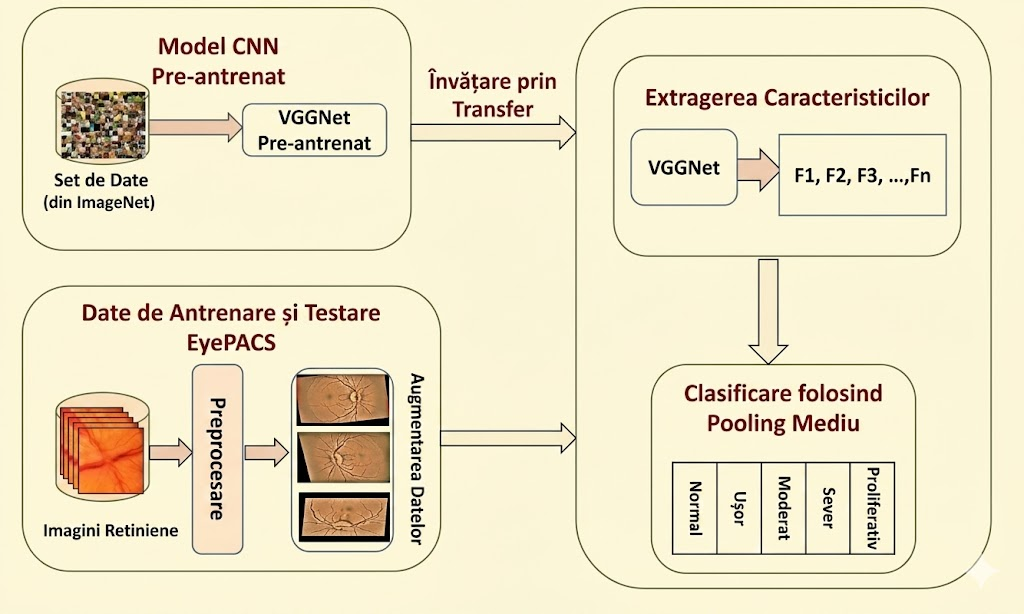
\includegraphics[width=1\columnwidth]{Figuri/Recommended_framework.png}
\captionsetup{justification=centering}
\caption{Framework propus pentru detectarea și clasificarea retinopatiei diabetice \cite{10_jabbar2022transfer}}
\label{fig: recommended-framework}
\end{figure}

\bigskip

Seturile de date utilizate includ imagini fundus publice din Kaggle EyePACS \cite{9_chetoui2020explainable}, preprocesate prin
redimensionare, normalizare și augmentare extensivă a datelor. Tehnicile de augmentare, precum
rotațiile, flip-urile orizontale și ajustările de luminozitate, joacă un rol central în creșterea diversității
artificiale a datelor și în îmbunătățirea capacității de generalizare a modelelor. Această etapă este
esențială în contextul “transfer learning-ului”, unde diferențele de distribuție dintre datele naturale și
imaginile medicale pot afecta performanța rețelelor \cite{10_jabbar2022transfer}.
\bigskip

Evaluarea performanței este realizată folosind metrici standard, precum acuratețea,
sensibilitatea, specificitatea și scorul F1, permițând o comparație riguroasă între diferitele arhitecturi
analizate. Rezultatele experimentale indică faptul că modelele bazate pe DenseNet și ResNet obțin
performanțe superioare față de arhitecturile mai vechi, confirmând avantajele reutilizării caracteristicilor
vizuale generale în sarcini medicale specializate. Studiul subliniază că transfer learning-ul reprezintă o
soluție viabilă și eficientă pentru implementarea rapidă a sistemelor automate de screening în contexte
cu resurse limitate \cite{10_jabbar2022transfer}.

\section{“Multi-task Learning” pentru gradarea retinopatiei diabetice \cite{6_wang2021deep}}

\ \ \ \ Lucrarea propusă de Wang et al. \cite{6_wang2021deep} introduce o abordare de tip
“deep multi-task learning”
pentru gradarea automată a retinopatiei diabetice, având ca obiectiv principal exploatarea relației clinice
dintre severitatea bolii și prezența leziunilor retiniene specifice. Spre deosebire de metodele clasice de
clasificare “single-task”, autorii demonstrează că învățarea simultană a mai multor sarcini corelate clinic
conduce la reprezentări vizuale mai discriminative și la performanțe superioare în sarcina principală de
gradare \cite{6_wang2021deep}.
\bigskip

Arhitectura propusă este alcătuită dintr-un backbone convoluțional comun, bazat pe o rețea CNN
profundă (ResNet18), utilizat pentru extracția caracteristicilor globale din imaginile fundus. Peste acest
extractor comun sunt construite mai multe ramuri specializate (task-specific branches), fiecare 
corespunzătoare unei sarcini distincte. Sarcina principală constă în clasificarea severității retinopatiei
diabetice în mai multe stadii, în timp ce sarcinile auxiliare vizează detectarea prezenței diferitelor tipuri
de leziuni, precum microanevrismele, exudatele dure, exudatele moi și hemoragiile, considerate
“markeri” clinici relevanți ai progresiei bolii \cite{6_wang2021deep}.
\bigskip

Un element central al arhitecturii îl reprezintă mecanismul de partajare controlată a
caracteristicilor între sarcini. În locul unei separări rigide între ramuri, modelul permite propagarea
informației relevante între sarcina de gradare și cele de detecție a leziunilor, încurajând învățarea unor
reprezentări comune sensibile la semnalele patologice fine. Funcția de pierdere globală este definită ca o
combinație ponderată a pierderilor individuale asociate fiecărei sarcini:

$$L_{isr} = \lambda_{img} \cdot L_{img\_isr} + \lambda_{tv} \cdot L_{tv\_isr} + \lambda_{sa} \cdot
L_{seg\text{-}aware} + \lambda_{ca} \cdot L_{cls\text{-}aware}$$
\bigskip

,unde $\lambda_{img}$, $\lambda_{tv}$, $\lambda_{sa}$ și $\lambda_{ca}$ sunt hiperparametri care controlează 
contribuția pierderilor ``intra-task'', ``segmentation-aware'' și ``classification-aware''. Această formulare permite echilibrarea
influenței fiecărei sarcini și stabilizează procesul de optimizare \cite{6_wang2021deep}.

Modelul este antrenat și evaluat pe seturi de date publice de imagini fundus etichetate (DDR
\cite{15_li2019diagnostic} și EyePACS \cite{9_chetoui2020explainable}) atât cu stadiul retinopatiei diabetice, cât și cu adnotări la nivel de imagine privind
prezența leziunilor. Imaginile sunt supuse unor etape standard de preprocesare, incluzând decuparea
regiunii retiniene, redimensionarea și augmentarea datelor, pentru a reduce variațiile de iluminare și
pentru a îmbunătăți capacitatea de generalizare. Prin includerea sarcinilor auxiliare, modelul beneficiază
de un efect de regularizare implicită, reducând riscul de supraînvățare, aspect observat și în lucrările
anterioare bazate pe CNN-uri “single-task” \cite{3_gulshan2016development}, \cite{4_pratt2016convolutional}.
\bigskip

Rezultatele experimentale raportate în articol indică îmbunătățiri consistente ale performanței
față de modelele “single-task”, atât în termeni de acuratețe, cât și de
scor F1 pentru sarcina de gradare a
retinopatiei diabetice. În plus, autorii evidențiază o creștere a stabilității predicțiilor și o sensibilitate mai
bună la stadiile intermediare ale bolii, considerate dificil de clasificat. Aceste rezultate confirmă faptul că
integrarea informațiilor despre leziuni în procesul de antrenare contribuie direct la o evaluare mai
precisă a severității retinopatiei diabetice și validează eficiența paradigmei “multi-task learning” în
context clinic \cite{6_wang2021deep}.
\bigskip

\section{Analiza arhitecturii “Modified U-Net” pentru segmentarea semantică \cite{12_sambyal2020modified}}

\ \ \ \ Segmentarea semantică a structurilor retiniene, în special a rețelei vasculare și a
leziunilor
asociate retinopatiei diabetice, reprezintă o etapă critică în diagnosticarea automată, deoarece
modificările morfologice ale vaselor de sânge sunt adesea primii indicatori ai bolii.
Deși arhitectura UNet, introdusă inițial de Ronneberger
et al. \cite{5_ronneberger2015u} pentru segmentarea biomedicală, a devenit standardul de
aur în domeniu datorită structurii sale simetrice de tip “encoder-decoder”, aceasta prezintă limitări în
detectarea vaselor capilare foarte fine, pierzând informații spațiale esențiale în procesul de subeșantionare.
\bigskip

În studiul "Modified U-Net architecture for semantic segmentation of diabetic retinopathy
images", Sambyal et al \cite{12_sambyal2020modified}. propun o optimizare arhitecturală semnificativă pentru a contracara aceste
deficiențe. Modelul propus, denumit Modified U-Net, păstrează structura în formă de „U” a rețelei
originale, dar inovează fundamental la nivelul blocurilor de procesare.
\bigskip

Autorii au înlocuit blocurile convoluționale standard cu blocuri reziduale (residual blocks),
inspirate din arhitecturile de tip ResNet. Această modificare este crucială din punct de vedere tehnic: în
rețelele adânci, apare frecvent problema dispariției gradientului (vanishing gradient), ceea ce face
antrenarea dificilă și duce la pierderea detaliilor fine. Prin introducerea conexiunilor reziduale (“skip
connections” la nivel de bloc), informația originală este propagată mai eficient prin straturi, permițând
rețelei să învețe caracteristici complexe fără a degrada performanța pe detaliile de finețe, precum
microanevrismele sau vasele subțiri. Aceste detalii se pot observa și în figura următoare.

\begin{figure}[h]
\centering
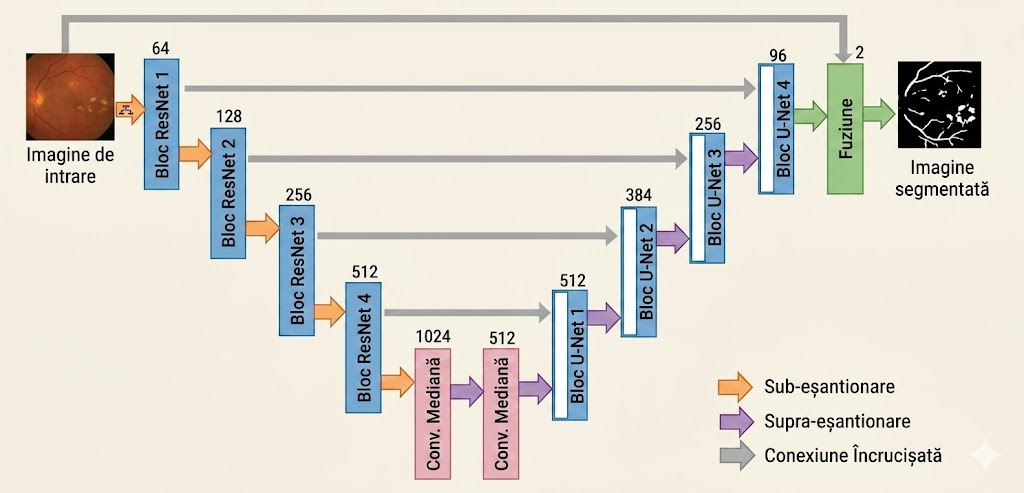
\includegraphics[width=1\columnwidth]{Figuri/modified-u-net.png}
\captionsetup{justification=centering}
\caption{Arhitectura U-net modificată \cite{12_sambyal2020modified}}
\label{fig: modified-u-net}
\end{figure}

\bigskip

Importanța acestei abordări constă în capacitatea de generalizare comparativ cu metodele
clasice de procesare a imaginii, precum cele bazate pe “clustering fuzzy” propuse anterior de Sopharak et
al. \cite{2_sopharak2009automatic}. În timp ce metodele de tip “clustering” sunt sensibile la
zgomot și la variațiile de iluminare
(frecvente în imaginile de fund de ochi), arhitectura Modified U-Net demonstrează o robustețe sporită
prin învățarea contextuală a trăsăturilor
\bigskip

Pentru validarea performanței, metoda a fost testată pe seturile de date publice standardizate
DRIVE \cite{13_staal2004ridge} și STARE \cite{9_chetoui2020explainable}, recunoscute pentru dificultatea lor în segmentarea vaselor.

Rezultatele experimentale raportate de Sambyal et al. \cite{12_sambyal2020modified} au indicat o îmbunătățire clară față de
U-Net-ul standard. Pe setul de date DRIVE, autorii au obținut o acuratețe
maximă de 96.94% și o arie de
sub curba ROC (AUC) de 0.98, valori care plasează metoda în topul
soluțiilor de segmentare. Mai mult,
analiza vizuală a rezultatelor arată o continuitate mult mai bună a vaselor
de sânge segmentate și o
reducere a alarmelor false în zonele cu patologii, demonstrând că integrarea învățării reziduale în
arhitectura de segmentare este o direcție esențială pentru analiza detaliată a retinopatiei diabetice.

\section{Tranziția către arhitecturi globale: RTNet (Relation Transformer Network) \cite{7_huang2022rtnet}}

\ \ \ \ Dacă modelele bazate pe U-Net, precum cel discutat anterior \cite{12_sambyal2020modified}, excelează în
capturarea
detaliilor locale, ele suferă totuși de o limitare inerentă a rețelelor convoluționale: incapacitatea de a
modela dependențe la distanță mare (long-range dependencies). În patologia retiniană, leziunile nu apar
izolat; există adesea o corelație spațială între poziția vaselor de sânge și apariția microanevrismelor sau a
exudatelor. Pentru a adresa această lipsă de „context global”, Huang et al.
\cite{7_huang2022rtnet} au propus în 2022 o
schimbare de paradigmă prin introducerea RTNet (Relation Transformer Network), o arhitectură care
marchează trecerea către mecanismele de atenție.
\bigskip

Inovația centrală a RTNet constă în înlocuirea parțială a operațiilor convoluționale standard cu
blocuri de tip “Transformer”, denumite Relation Transformer Blocks (RTB). Spre deosebire de CNN-uri
care „văd” doar o fereastră mică de pixeli la un moment dat,
RTB-ul utilizează două mecanisme de
atenție complementare:

\begin{enumerate}
  \item “Self-Attention” (Atenție proprie): Permite modelului să înțeleagă relațiile dintre leziunile
        dispersate pe toată suprafața retinei (de exemplu, grupuri de exudate dure care semnalează o
        zonă de edem).

\item “Cross-Attention” (Atenție încrucișată): Autorii au observat că leziunile vasculare sunt strâns
      legate de structura vaselor de sânge. Astfel, mecanismul de “cross-attention” folosește harta
      vaselor de sânge ca un „ghid” pentru a localiza mai precis leziunile fine, transferând informație
      structurală dinspre ramura vasculară către ramura de detectare a leziunilor.
\end{enumerate}
\bigskip

Pentru validare, metoda a fost testată pe seturile de date IDRiD \cite{9_chetoui2020explainable}
și DDR \cite{15_li2019diagnostic}, care conțin adnotări
la nivel de pixel pentru multiple tipuri de leziuni. Rezultatele cantitative au demonstrat că RTNet
depășește metodele existente anterioare (inclusiv diverse variante de U-Net și DeepLab), obținând cele
mai bune scoruri de segmentare pentru Exudate (EX), Microanevrisme (MA) și Exudate Moi (SE).
\bigskip

Deși inovația teoretică a arhitecturii RTNet (Relation Transformer Network) propusă de Huang et al.
\cite{7_huang2022rtnet} este evidentă prin integrarea mecanismelor de atenție, validarea practică a acesteia necesită o
demonstrație riguroasă a faptului că fiecare modul propus contribuie activ la îmbunătățirea segmentării.
În acest sens, autorii au realizat un studiu extensiv de ablație (ablation study), analizând impactul
incremental al componentelor arhitecturale asupra capacității de învățare și generalizare a rețelei.
\bigskip

Această analiză comparativă este sintetizată în graficele de performanță care monitorizează evoluția
funcției de pierdere (Loss) și curbele Precision-Recall (PR) pentru cele patru tipuri principale de leziuni
asociate retinopatiei diabetice: microanevrisme (MA), exudate (EX), hemoragii (HE) și exudate moi (SE).
\bigskip

Comparatia pornește de la un model “Baseline” (o rețea convoluțională standard de tip U-Net fără
mecanisme de atenție) și adaugă progresiv componentele specifice RTNet, regasite în figura de mai jos:

\begin{enumerate}
  \item GTB (Global Transformer Block): Adăugarea capacității de procesare globală.
  \item SAH (Self-Attention Head): Introducerea atenției proprii pentru corelarea leziunilor similare.
  \item RAH (Relation Attention Head / Cross-Attention): Modulul critic care leagă leziunile de structura
vaselor de sânge.
  \item RTB (Relation Transformer Block): Arhitectura completă propusă.
\end{enumerate}

\begin{figure}[h]
\centering
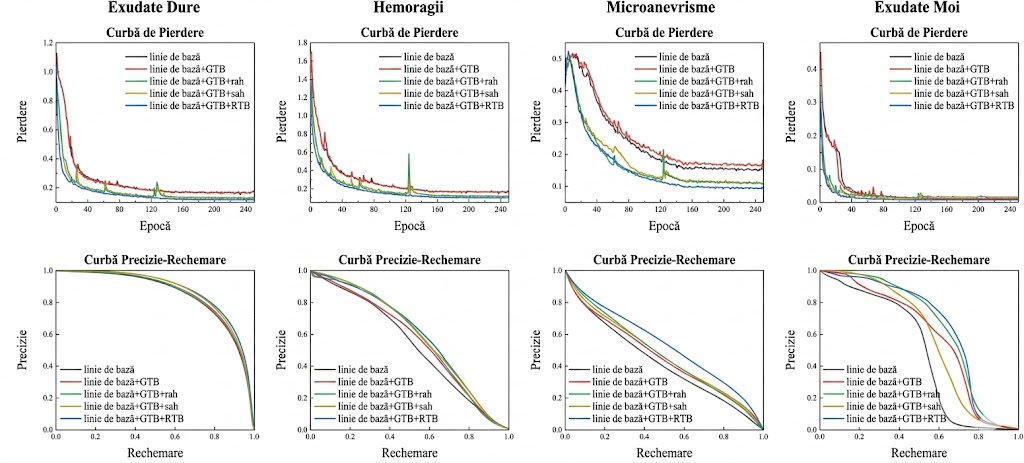
\includegraphics[width=1\columnwidth]{Figuri/loss-curves-ablations.png}
\captionsetup{justification=centering}
\caption{Curbele de Loss (stânga) și curbele Precision-Recall (dreapta) pentru studiile de ablație asupra celor patru leziuni DR. \cite{7_huang2022rtnet}}
\label{fig: loss-curves}
\end{figure}
\bigskip

Lucrarea lui Huang et al. \cite{7_huang2022rtnet} validează ipoteza că integrarea informației globale prin Transformere
este pasul necesar pentru a depăși plafonul de performanță atins de rețelele convoluționale pure în
segmentarea medicală complexă.

\section{Arhitectura “Dual Branch” \cite{11_shakibania2024dual}}

\ \ \ \ Deși progresele în segmentarea semantică, ilustrate prin metodele bazate pe U-Net \cite{12_sambyal2020modified}
sau pe
Transformere \cite{7_huang2022rtnet}, au permis o delimitare precisă a leziunilor, translatarea acestor detalii într-un
diagnostic global (grading) rămâne o provocare majoră din cauza naturii subtile a diferențelor dintre
stadiile retinopatiei diabetice. Rețelele convoluționale standard utilizate în studiile fundamentale,
precum cel al lui Gulshan et al. \cite{3_gulshan2016development}, tind să piardă detaliile
fine, cum ar fi microanevrismele incipiente, în
procesul de redimensionare a imaginii necesar pentru analiza globală. Pentru a depăși acest compromis
inerent între contextul vizual și rezoluția detaliilor, Shakibania et al. \cite{11_shakibania2024dual} au propus o arhitectură
inovatoare de tip “Dual Branch Deep Learning Network”, care restructurează procesul de învățare prin
decuplarea extragerii trăsăturilor în două fluxuri paralele distincte.

Conceptul central al acestei abordări constă în imitarea procesului cognitiv uman de
diagnosticare, procesând imaginea simultan pe o „ramură globală” și o „ramură locală”. Ramura globală
analizează imaginea completă a fundului de ochi pentru a captura structura generală a vaselor și
geometria retinei, o strategie similară cu metodele clasice de “Transfer Learning” \cite{10_jabbar2022transfer}. În paralel, ramura
locală operează pe decupaje de înaltă rezoluție, fiind specializată în identificarea leziunilor microscopice 
care ar fi invizibile pentru rețeaua globală. Elementul de noutate adus de această lucrare față de
abordările “multi-task” anterioare \cite{6_wang2021deep}, este mecanismul de fuziune a celor două fluxuri, care utilizează
tehnici de atenție pentru a pondera importanța trăsăturilor locale în decizia finală, asigurând că un
detaliu critic nu este ignorat în favoarea unei imagini de ansamblu aparent sănătoase.

Eficiența acestei arhitecturi hibride este validată prin rezultatele experimentale obținute pe
seturile de date standard, unde modelul “Dual Branch” a demonstrat o superioritate clară în clasificarea
stadiilor intermediare ale bolii (ușor și moderat). Analiza performanței indică faptul că integrarea
informației locale crește semnificativ sensibilitatea modelului și reduce confuzia între clasele adiacente,
oferind o robustețe superioară la variațiile de calitate a imaginii comparativ cu
arhitecturile “singlestream”. Astfel, lucrarea confirmă faptul că performanța actuală în 2024 nu
derivă doar din adâncimea
rețelei, ci din capacitatea arhitecturală de a reuni viziunea macroscopică cu cea microscopică într-un
diagnostic coerent.

\section{Abordarea “Explainable AI” \cite{9_chetoui2020explainable}}

\ \ \ \ În timp ce arhitecturile precum “Dual Branch Network” \cite{11_shakibania2024dual} sau Transformer-ele relaționale
\cite{7_huang2022rtnet}
au reușit să împingă limitele acurateței și ale segmentării fine, integrarea acestor sisteme în fluxul clinic
real se lovește de o barieră fundamentală: lipsa de încredere a medicilor
în algoritmii de tip „black-box”.
Validarea clinică inițiată de Gulshan et al. \cite{3_gulshan2016development} a demonstrat potențialul diagnostic, însă pentru ca un
sistem de inteligență artificială să fie acceptat ca asistent de încredere, acesta trebuie să își poată
justifica deciziile. În acest context, lucrarea publicată de Chetoui și Akhloufi \cite{9_chetoui2020explainable}, reprezintă un pilon
esențial al stadiului actual al cunoașterii, adresând simultan două probleme critice: interpretabilitatea
(Explainable AI - XAI) și robustețea pe seturi de date eterogene.
\bigskip

Metodologia propusă de autori se bazează pe o arhitectură de tip CNN modificată (utilizând
backbone-uri precum DenseNet121 sau ResNet50), în care straturile clasice complet conectate sunt
înlocuite cu Global Average Pooling (GAP). Această modificare tehnică permite generarea Hărților de
Activare a Claselor (CAM), oferind medicului o confirmare vizuală a regiunilor patologice care au
determinat diagnosticul.
\bigskip

Relevanța clinică a acestei abordări extensive este evidențiată în rezultatele vizuale, unde hărțile
de saliență generate de algoritm se suprapun cu precizie peste semnele patologice reale, indiferent de
setul de date din care provine imaginea. Zonele marcate cu roșu intens pe hărțile CAM corespund
anatomic cu microanevrismele și exudatele, confirmând că rețeaua neuronală a învățat trăsăturile
intrinseci ale bolii și nu caracteristicile specifice ale camerei foto (bias-ul echipamentului). Prin urmare,
modelul propus \cite{9_chetoui2020explainable} validează faptul că un sistem trebuie să fie nu
doar precis, ci și independent de sursa
datelor și transparent în decizii.

\section{Generalizarea în scenarii reale: “Multi-Model Domain Adaptation” \cite{8_zhang2022multi}}

\ \ \ \ Ultima frontieră în dezvoltarea sistemelor de diagnostic asistat de calculator (CAD) pentru
retinopatia diabetică nu mai este legată strict de acuratețea obținută pe un
singur set de date de
antrenament, ci de capacitatea algoritmului de a funcționa corect într-un mediu clinic eterogen. În
realitate, imaginile de fund de ochi variază drastic în funcție de modelul camerei, setările de iluminare,
etnia pacientului sau protocolul de achiziție, fenomen cunoscut sub numele de “domain shift”. Modelele
antrenate pe un „domeniu sursă” (de exemplu, imagini de înaltă calitate de
la EyePACS \cite{9_chetoui2020explainable}) tind să aibă
performanțe scăzute atunci când sunt aplicate pe un „domeniu țintă” (imagini clinice noi, cu
caracteristici vizuale diferite), ceea ce limitează sever aplicabilitatea lor universală.
\bigskip

Pentru a soluționa această problemă critică de implementare, Zhang et al. \cite{8_zhang2022multi} au propus în 2022
o metodă inovatoare denumită “Multi-Model Domain Adaptation” (MMDA). Spre deosebire de
abordările anterioare care încearcă să alinieze domeniile folosind un singur model, autorii introduc o
arhitectură complexă bazată pe o rețea siameză, utilizând două modele distincte pentru a extrage
trăsături complementare și pentru a crește robustețea deciziei.
\bigskip

Inovația tehnică centrală a lucrării constă în integrarea simultană a trei mecanisme de optimizare
care lucrează concertat pentru a forța modelul să ignore diferențele stilistice dintre
seturile de date și să
se concentreze exclusiv pe patologie. Astfel, arhitectura combină o pierdere de clasificare pentru a
asigura acuratețea diagnostică pe domeniul sursă etichetat, cu o pierdere de discrepanță care
maximizează diferența dintre predicțiile celor două clasificatore pe domeniul țintă pentru a detecta
exemplele aflate la granița de decizie. În plus, se utilizează o pierdere
de adaptare adversarială care, prin
intermediul unui discriminator, minimizează distanța dintre distribuția trăsăturilor din sursă și cea din
țintă, făcând ca imaginile provenite din spitale diferite să fie reprezentate similar de către rețeaua
neuronală.
\bigskip

Validarea experimentală a metodei a fost realizată folosind setul de date EyePACS \cite{9_chetoui2020explainable} ca domeniu
sursă și Messidor-2 \cite{9_chetoui2020explainable} ca domeniu țintă, simulând un scenariu realist de
transfer tehnologic de la imagini
de screening la imagini clinice de referință. Rezultatele au demonstrat că abordarea MMDA depășește
semnificativ metodele standard de antrenare și alte tehnici de adaptare cunoscute, obținând o
îmbunătățire substanțială a metricilor de performanță pe domeniul țintă fără a necesita etichete pentru
acesta. Această lucrare încheie logic analiza stadiului actual al cunoașterii, subliniind faptul că un sistem
complet nu trebuie doar să segmenteze leziuni fine sau să fie explicabil,
ci trebuie să fie capabil să iasă
din mediul controlat al laboratorului și să ofere o performanță robustă și generalizabilă în diversele
condiții întâlnite în practica medicală globală.

\section{Concluzii}

\ \ \ \ Analiza literaturii de specialitate relevă faptul că detectarea automată a retinopatiei diabetice
a
depășit stadiul de experiment teoretic, devenind o direcție de cercetare matură, cu rezultate clinice
valide. Totuși, problema rămâne una de o complexitate ridicată, care depășește simpla clasificare a
imaginilor. Dificultatea majoră nu constă doar în volumul masiv de date necesar, ci în subtilitatea
semnelor patologice incipiente, precum microanevrismele, care pot ocupa doar câțiva pixeli dintr-o
imagine de înaltă rezoluție, fiind ușor de confundat cu artefactele sau zgomotul de fond. Această
granularitate fină impune algoritmilor o capacitate de discriminare vizuală care, în anumite scenarii
limită, trebuie să depășească acuitatea ochiului uman.
\bigskip

În ciuda acestor obstacole, soluțiile algoritmice existente demonstrează o evoluție remarcabilă.
Trecerea de la rețelele convoluționale standard la arhitecturi sofisticate, capabile să integreze informația
globală cu cea locală prin mecanisme de tip “dual-branch” \cite{11_shakibania2024dual}, a permis o creștere semnificativă a
sensibilității în detectarea stadiilor intermediare ale bolii. Mai mult, rezultatele obținute prin tehnici de
adaptare la domeniu \cite{8_zhang2022multi} sugerează că bariera variabilității echipamentelor medicale începe să fie
depășită, deschizând calea pentru sisteme robuste, capabile să funcționeze corect indiferent de spitalul
în care sunt implementate.
\bigskip

Un alt aspect promițător este schimbarea de paradigmă de la modelele de tip „cutie neagră” la
sistemele explicabile (Explainable AI). Așa cum evidențiază studiile recente \cite{9_chetoui2020explainable}, capacitatea modelelor de
a genera hărți de activare precise transformă inteligența artificială dintr-un simplu clasificator statistic
într-un partener transparent pentru medic, facilitând validarea rapidă a deciziei. Deși provocările legate
de dezechilibrul claselor și de generalizarea pe populații diverse persistă, performanțele atinse de
metodele actuale, validate pe seturi de date riguroase precum MESSIDOR-2 \cite{9_chetoui2020explainable}, confirmă potențialul
acestor tehnologii de a eficientiza screening-ul în masă și de a preveni orbirea la scară globală.


\chapter{Seturi de date și construirea dataset-urilor experimentale}

\section{Rolul seturilor de date în lucrare}

\ \ \ \ Clasificarea automată a retinopatiei diabetice depinde puternic de calitatea imaginilor,
de distribuția claselor și de modul în care datele sunt separate înainte de antrenare. În
literatură, diferențele dintre seturi precum EyePACS, APTOS, DDR, IDRiD sau Messidor sunt
discutate frecvent în raport cu robustețea modelelor și cu problema schimbării domeniului
vizual (\textit{domain shift}) \cite{3_gulshan2016development}, \cite{8_zhang2022multi},
\cite{9_chetoui2020explainable}, \cite{14_liu2022deepdrid}, \cite{15_li2019diagnostic}.
Din acest motiv, în această lucrare seturile de date nu au fost tratate ca simple directoare
de imagini, ci ca o componentă de metodologie centrală a sistemului.
\bigskip

O parte importantă a lucrării a constat în construirea, curățarea și verificarea mai multor
variante de seturi de date. Imaginile au fost reorganizate local, filtrate, împărțite în subseturi,
augmentate și preprocesate prin fluxuri reproductibile. Acest efort a fost necesar deoarece
rezultate aparent foarte bune pot fi obținute artificial atunci când imagini derivate din
aceeași sursă ajung simultan în antrenare și în validare sau testare. În consecință, capitolul
prezintă nu doar sursele de date, ci și munca practică realizată pentru a transforma aceste
surse în seturi experimentale controlate.
\bigskip

Pașii urmăriți în construirea dataset-urilor au fost:

\begin{itemize}
  \item identificarea și descărcarea surselor publice relevante pentru clasificarea retinopatiei diabetice;
  \item verificarea structurii inițiale a fiecărui set și numărarea imaginilor pe clase;
  \item reorganizarea imaginilor într-un format comun \texttt{train}/\texttt{val}/\texttt{test}, fiecare subset fiind împărțit în clasele 0-4;
  \item curățarea imaginilor invalide, foarte neclare sau fără regiune retiniană detectabilă;
  \item aplicarea augmentărilor doar pe subsetul de antrenare;
  \item generarea variantelor preprocesate prin metoda Ben Graham;
  \item verificarea riscului de \textit{data leakage}, mai ales în seturile care conțin augmentări preexistente. 
\end{itemize}
\bigskip

Au fost folosite mai multe surse de date: EyePACS, APTOS 2019, \texttt{Diabetic\_Balanced\_Data}
și \texttt{Diabetic\_Balanced\_Aug}. Modelul principal al lucrării este construit pe EyePACS,
într-un pipeline local CUDA, iar celelalte seturi au fost folosite pentru experimente
preliminare, comparații între arhitecturi și analiza robustă a protocolului de evaluare.
Toate variantele finale au fost aduse, pe cât posibil, la o structură comună de tip:

\begin{center}
\small
\begin{verbatim}
dataset/
  train/0  train/1  train/2  train/3  train/4
  val/0    val/1    val/2    val/3    val/4
  test/0   test/1   test/2   test/3   test/4
\end{verbatim}
\end{center}

Clasele numerice corespund celor cinci niveluri clinice ale retinopatiei diabetice: clasa 0
reprezintă absența bolii, clasa 1 forma ușoară, clasa 2 forma moderată, clasa 3 forma severă,
iar clasa 4 forma proliferativă.

\section{Sursele de date utilizate}

\ \ \ \ Setul EyePACS a fost utilizat ca sursă principală pentru sistemul final. Acesta conține
un număr mare de imagini de fund de ochi, dar are o distribuție puternic dezechilibrată:
clasa 0 este dominantă, în timp ce clasele severe sunt mult mai puțin reprezentate.
Dezechilibrul este o caracteristică întâlnită frecvent în screening-ul pentru retinopatie
diabetică, unde imaginile normale sau cazurile moderate apar mai des decât formele severe
\cite{3_gulshan2016development}, \cite{15_li2019diagnostic}. Tocmai din acest motiv, EyePACS
este relevant pentru scenarii apropiate de practica reală, dar impune atenție la metricile
folosite și la strategia de antrenare.
\bigskip

Setul APTOS 2019 a fost folosit pentru experimente comparative și pentru analiza efectului
augmentării și al preprocesării Ben Graham. Imaginile APTOS provin dintr-o distribuție diferită
de EyePACS, astfel încât ele permit observarea sensibilității modelelor la schimbarea
domeniului vizual. Această diferență de domeniu este importantă deoarece modelele antrenate
pe un singur set pot învăța particularități ale camerei, iluminării sau rezoluției, nu doar
semne clinice ale bolii \cite{8_zhang2022multi}, \cite{9_chetoui2020explainable}.
\bigskip

Din punct de vedere experimental, APTOS este valoros deoarece are un volum mai redus decât
EyePACS, dar imagini relativ bine standardizate și etichete pe aceeași scară de severitate
0--4, făcandu-l fiabil pentru experimente rapide și eficiente. Prin urmare, el a fost folosit 
ca set de test pentru deciziile de preprocesare și augmentare: dacă o strategie funcționează 
doar pe un dataset mare, dar nu se păstrează pe APTOS, atunci există riscul ca modelul să fi 
învățat particularități ale sursei, nu trăsături generale ale retinopatiei diabetice.
\bigskip

Setul \texttt{Diabetic\_Balanced\_Data}, disponibil public pe Kaggle sub denumirea
\textit{Diabetic Retinopathy Balanced} \cite{24_kaggle_diabetic_balanced}, a fost folosit în
experimentele inițiale de comparație între arhitecturi, funcții de pierdere și optimizatori.
Ulterior, analiza acestui set a devenit importantă metodologic, deoarece s-a observat că
organizarea sa poate permite apariția unui \textit{data leakage} între subseturi. 
\bigskip

Setul \texttt{Diabetic\_Balanced\_Aug} a fost folosit ca sursă mare, dezechilibrată, din care au
fost construite mai multe variante: split inițial, variantă curățată, variantă augmentată și
variantă augmentată cu preprocesare Ben Graham. Aceste variante au fost generate prin
scripturile din directorul \path{Scripts/Diabetic_Balanced_Aug}.
\bigskip

Prin folosirea acestor surse complementare, lucrarea a urmărit două obiective practice:

\begin{itemize}
  \item obținerea unui set principal suficient de mare pentru antrenarea modelelor CNN prin \textit{transfer learning};
  \item testarea deciziilor de preprocesare și organizare pe seturi cu distribuții și niveluri de calitate diferite.
\end{itemize}

\section{Pipeline-ul de prelucrare pentru EyePACS}

\ \ \ \ Pentru EyePACS au fost create mai multe variante experimentale prin scripturile din
\path{Scripts/EyePACS}. Primul pas este realizat de notebook-ul \path{split_eyepacs.ipynb},
care citește fișierele CSV cu etichete, caută imaginile existente în directorul
\path{Images}, păstrează doar intrările care pot fi mapate corect și creează o împărțire
stratificată în subseturile \texttt{train}, \texttt{val} și \texttt{test}. Imaginile sunt apoi
copiate în directoare numerotate de la 0 la 4, corespunzătoare claselor.
\bigskip

Al doilea pas este curățarea imaginilor, implementată în \path{clean_eyepacs.ipynb}. Scriptul
verifică fiecare imagine printr-un set de criterii simple de calitate: citirea corectă a
fișierului, claritatea estimată prin varianța Laplacianului, existența unei regiuni retiniene
detectabile prin threshold și contur, precum și aria regiunii principale. Imaginile valide
sunt copiate în \texttt{eyepacs\_cleaned}.
\bigskip

Algoritmul de curățare a fost construit ca un filtru automat, aplicat înainte de augmentare și
preprocesare. Logica urmărită este următoarea:

\begin{itemize}
  \item \textbf{Redimensionarea pentru analiză:} imaginea este adusă temporar la o dimensiune standard, astfel încât pragurile de claritate și de arie să fie comparabile între fișiere.
  \item \textbf{Conversia în grayscale:} imaginea este convertită în tonuri de gri pentru a analiza intensitatea globală și pentru a separa mai ușor retina de fundal.
  \item \textbf{Estimarea clarității:} se calculează varianța Laplacianului; valori foarte mici indică imagini încețoșate, din care modelul poate învăța trăsături instabile.
  \item \textbf{Detectarea regiunii retiniene:} se aplică un prag de intensitate pentru separarea fundului de ochi de fundalul negru, apoi se caută contururile rezultate.
  \item \textbf{Validarea conturului principal:} este păstrat cel mai mare contur, presupus a fi regiunea retiniană; imaginile fără contur sau cu o arie prea mică sunt respinse.
\end{itemize}
\bigskip

Prin această succesiune de pași, curățarea nu modifică diagnosticul și nu introduce imagini noi,
ci elimină intrările care ar putea afecta negativ antrenarea: imagini neclare, imagini aproape
goale, imagini cu fund de ochi foarte mic sau fișiere imposibil de citit. Această etapă a fost
aplicată înaintea augmentării tocmai pentru ca imaginile sintetizate să pornească din exemple
valide, nu din imagini problematice.
\bigskip

Această etapă a avut rolul de a elimina cazurile în care imaginea nu putea fi folosită în mod
fiabil de model: fișiere corupte, imagini aproape complet întunecate, imagini cu fund de ochi
foarte mic în cadru sau imagini în care conturul retinian nu putea fi separat suficient de
fundal. În analiza imaginilor medicale, calitatea intrării influențează direct capacitatea
modelului de a învăța trăsături utile \cite{14_liu2022deepdrid}.
\bigskip

Pentru reducerea dezechilibrului de clase, notebook-ul \path{form_eyepacs_augmented.ipynb}
generează o variantă augmentată. Scriptul copiază imaginile originale și aplică augmentări
doar pe subsetul de antrenare: flip, transformări afine, blur gaussian, variații moderate
de luminozitate/contrast și zgomot. Scopul nu este modificarea diagnosticului, ci creșterea
diversității vizuale pentru clasele minoritare.
\bigskip

În alegerea augmentărilor s-a urmărit păstrarea sensului clinic al imaginii. Astfel, transformările
au fost limitate la modificări care pot simula variații obișnuite de achiziție, fără a introduce
artefacte agresive. Pentru retinopatia diabetică, această precauție este importantă deoarece
leziunile relevante pot fi mici, iar o augmentare excesivă poate estompa microanevrismele,
hemoragiile punctiforme sau exudatele \cite{1_niemeijer2005automatic}, \cite{2_sopharak2009automatic}.
\bigskip

Augmentarea a avut trei roluri practice. În primul rând, a crescut numărul de exemple pentru
clasele slab reprezentate, reducând tendința modelului de a favoriza clasa majoritară. În al
doilea rând, a expus rețeaua la variații de poziție, scară, luminozitate și claritate asemănătoare
celor întâlnite între camere sau sesiuni diferite de achiziție. În al treilea rând, a permis
compararea între variante de dataset fără a schimba arhitectura modelului, astfel încât efectul
preprocesării și al augmentării să poată fi analizat separat. Pentru a păstra validitatea
evaluării, imaginile din validare și test nu au fost augmentate artificial.
\bigskip

Ultima variantă este generată de \path{form_eyepacs_augmented_bengraham.ipynb}, care aplică
preprocesarea Ben Graham peste imaginile augmentate. Astfel se obține un set în care
fundalul, contrastul și regiunea retiniană sunt mai uniformizate.

\section{Pipeline-ul de prelucrare pentru APTOS 2019}

\ \ \ \ Setul APTOS 2019 a fost prelucrat printr-un flux asemănător cu cele folosite pentru
EyePACS și \texttt{Diabetic\_Balanced\_Aug}. Imaginile au fost reorganizate pe clase, apoi au
fost construite variante experimentale cu augmentare și cu preprocesare Ben Graham. Scopul nu
a fost doar creșterea numerică a setului, ci obținerea unui banc de testare mai controlat pentru
efectul preprocesărilor.
\bigskip

În cazul APTOS, augmentările au fost importante deoarece setul este mai mic decât EyePACS, iar
clasele severe au mai puține exemple disponibile. Au fost folosite transformări moderate:
flip-uri, rotații mici, scalări, modificări de luminozitate și contrast, blur ușor și zgomot
gaussian. Aceste transformări simulează variații reale ale achiziției, dar evită deformarea
patologiei. Astfel, modelul este încurajat să recunoască structuri retiniene relevante, nu
poziții fixe sau caracteristici accidentale ale imaginilor.
\bigskip

După augmentare, au fost generate și variante preprocesate prin metoda Ben Graham. Această etapă
a uniformizat iluminarea, a redus influența fundalului și a făcut mai vizibile structurile
retiniene. Prin folosirea aceluiași tip de preprocesare ca în celelalte dataset-uri, APTOS a
devenit util pentru experimente comparative: se poate observa dacă modelul reacționează similar
pe o distribuție diferită sau dacă performanța depinde de sursa imaginilor.
\bigskip

APTOS a fost, așadar, un dataset experimental potrivit pentru lucrare din patru motive:

\begin{itemize}
  \item dimensiunea sa mai redusă, dar totuși în același timp echilibrată și cu imagini curate
  \item are aceeași formulare multiclasă 0--4 ca celelalte seturi folosite;
  \item provine dintr-un domeniu vizual diferit, util pentru testarea robusteții;
  \item permite analiza separată a efectului augmentării și al preprocesării Ben Graham pe un set mai mic și mai controlabil.
\end{itemize}

\section{Pipeline-ul de prelucrare pentru Diabetic\_Balanced\_Aug}

\ \ \ \ Pentru \texttt{Diabetic\_Balanced\_Aug}, fluxul este similar și este implementat în
\path{Scripts/Diabetic_Balanced_Aug}. Notebook-ul \path{split_balanced_aug.ipynb} citește
\texttt{trainLabels.csv}, potrivește etichetele cu imaginile din \path{resized_train} și
creează un split stratificat pe clase.
\bigskip

Notebook-ul \path{clean_balanced_aug.ipynb} construiește varianta \texttt{balanced\_aug\_cleaned}.
\newline
Acesta aplică filtre de calitate asemănătoare cu cele folosite pentru EyePACS: verificarea
citirii imaginii, redimensionarea pentru analiză, estimarea clarității, segmentarea aproximativă
a fundului de ochi și validarea conturului principal.
\bigskip

Pentru acest set, curățarea a fost utilă deoarece imaginile provin dintr-o colecție deja
prelucrată și nu toate fișierele au aceeași calitate vizuală. Prin aplicarea acelorași criterii
ca în cazul EyePACS, s-a obținut un protocol comparabil între dataset-uri. Această uniformizare
nu elimină complet diferențele dintre surse, dar reduce variațiile produse de organizarea locală
a fișierelor.
\bigskip

În practică, același algoritm de curățare a avut două efecte importante asupra acestui dataset:

\begin{itemize}
  \item a separat etapa de control al calității de etapa de augmentare, ceea ce a permis compararea clară între dataset-ul curățat și dataset-ul augmentat;
  \item a redus riscul ca imaginile cu fundal dominant, contur incorect sau blur puternic să fie multiplicate prin augmentări și să influențeze disproporționat antrenarea.
\end{itemize}
\bigskip

Notebook-ul \path{form_balanced_augmented.ipynb} creează varianta \texttt{balanced\_augmented}.
Pentru fiecare clasă, imaginile originale din train sunt păstrate, iar clasele minoritare sunt
completate prin augmentări generate dinamic. Transformările includ flip, rotații și scalări
mici, blur, variații de culoare și zgomot gaussian. Subseturile de validare și testare sunt
copiate fără augmentări suplimentare, pentru a păstra evaluarea stabilă.
\bigskip

Pentru acest dataset, augmentarea a fost tratată ca o etapă de construcție a datelor, nu ca o
operație aplicată întâmplător în timpul evaluării. Prin generarea variantelor augmentate offline,
s-a putut verifica explicit câte imagini apar în fiecare clasă și în fiecare subset. Această
abordare a făcut mai ușoară compararea dintre setul curățat, setul augmentat și setul augmentat
cu Ben Graham.
\bigskip

În final, \path{form_balanced_augmented_bengraham.ipynb} aplică metoda Ben Graham și generează
\texttt{balanced\_augmented\_bengraham}. Această variantă a fost folosită pentru a observa dacă
uniformizarea iluminării și accentuarea contrastului local ajută modelele pe un set mai mare
și dezechilibrat.

\section{Verificarea distribuției imaginilor}

\ \ \ \ Pe lângă generarea efectivă a dataset-urilor, a fost realizată și o etapă de verificare
a distribuției imaginilor. În notebook-ul \path{Notebooks/teste_si_incercari.ipynb} au fost incluse
funcții pentru numărarea imaginilor pe clase și subseturi, aplicate succesiv pe variantele
intermediare și finale. Această verificare a fost importantă deoarece o eroare de copiere sau
o distribuție foarte diferită între \texttt{train}, \texttt{val} și \texttt{test} poate afecta
direct interpretarea rezultatelor, dând avantaj clasei majoritare.
\bigskip
\bigskip 

Pentru fiecare dataset au fost urmărite următoarele aspecte:

\begin{itemize}
  \item existența tuturor claselor în fiecare subset;
  \item numărul de imagini pe clasă după curățare și augmentare;
  \item păstrarea validării și testării fără augmentări generate artificial;
  \item compararea vizuală a imaginilor originale cu imaginile preprocesate;
  \item identificarea variantelor de dataset care pot fi folosite pentru experimente preliminare și a celor potrivite pentru sistemul final.
\end{itemize}

\section{Separarea originalelor de augmentări în Diabetic\_Balanced\_Data}

\ \ \ \ Un pas distinct a fost realizat pentru setul \texttt{Diabetic\_Balanced\_Data}. Scriptul
\path{Scripts/DIabetic_Balanced_Data/split_diabetic_balanced_augmented.py} separă imaginile
originale de cele augmentate pe baza markerului \texttt{\_aug\_} din numele fișierului.
Rezultatul constă în două colecții separate: una cu imagini originale și una cu imagini
augmentate. Această separare a fost necesară pentru a înțelege mai bine compoziția setului
și pentru a investiga dacă imaginile augmentate pot apărea în subseturi diferite față de
imaginea originală.
\bigskip

Din punct de vedere experimental, această etapă a fost una dintre cele mai importante, deoarece
a mutat accentul de la simpla antrenare a modelelor la validitatea datelor folosite. Într-un
dataset care include deja imagini augmentate, fișierele pot părea exemple independente, deși
ele provin din aceeași imagine inițială. Dacă aceste versiuni sunt distribuite aleator în
subseturi diferite, modelul poate recunoaște structuri aproape identice în validare sau testare.

\section{Controlul data leakage prin split grupat}

\ \ \ \ În ultimele experimente realizate pe \texttt{Diabetic\_Balanced\_Data} s-a observat o
problemă metodologică importantă: setul public de pe Kaggle poate produce rezultate artificiale 
dacă imaginile originale și augmentările lor sunt împărțite între subseturi diferite.
Această situație reprezintă \textit{data leakage}, deoarece modelul poate vedea în antrenare o
variantă foarte apropiată de o imagine care apare ulterior în validare sau testare.
\bigskip 


Pentru verificarea acestei ipoteze a fost creat scriptul
\path{Scripts/DIabetic_Balanced_Data/grouped_split_diabetic_balanced_data.py}. Scriptul grupează
fiecare imagine originală împreună cu augmentările sale, apoi împarte grupurile, nu fișierele
individuale, în \texttt{train}, \texttt{val} și \texttt{test}, folosind raportul 70\%/20\%/10\%.
După copiere, scriptul validează că niciun grup nu apare în mai multe subseturi și salvează
un raport în \path{grouped_split_report.json}.
\bigskip

\begin{figure}[H]
\centering
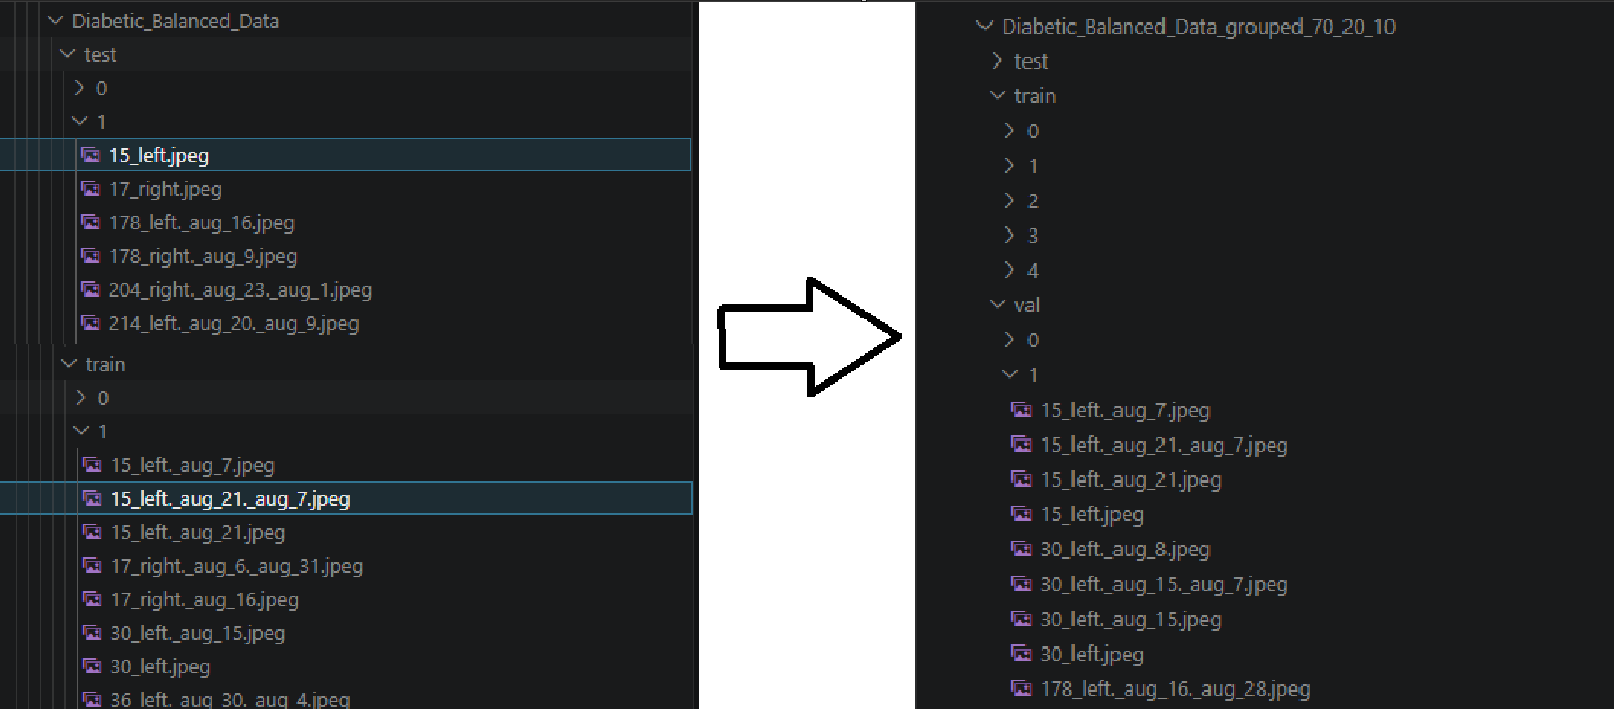
\includegraphics[width=0.95\textwidth]{Figuri/data_leakage_example_DBD.png}
\captionsetup{justification=centering}
\caption{Exemplu de data leakage în \texttt{Diabetic\_Balanced\_Data}: imaginea originală și augmentările sale apar în subseturi diferite, permițând modelului să recunoască structuri aproape identice în validare sau testare.}
\label{fig:data-leakage-example}
\end{figure}

Logica scriptului poate fi rezumată astfel:

\begin{itemize}
  \item se extrage numele imaginii de bază prin eliminarea markerilor de augmentare;
  \item toate fișierele care provin din aceeași imagine sunt plasate în același grup;
  \item împărțirea se face la nivel de grup, nu la nivel de fișier individual;
  \item după copiere se verifică intersecția grupurilor între subseturi;
  \item se salvează un raport care documentează numărul de imagini și grupuri rezultate.
\end{itemize}
\bigskip

Această descoperire este o contribuție practică a lucrării. Ea arată că performanțele obținute
pe seturi publice trebuie interpretate împreună cu modul exact de împărțire a datelor. În
capitolul de rezultate se arată că, după eliminarea acestui risc de \textit{data leakage},
performanța scade semnificativ, ceea ce confirmă că evaluarea inițială era prea optimistă.

\section{Preprocesarea Ben Graham}

\ \ \ \ Preprocesarea Ben Graham este folosită pentru reducerea variațiilor de iluminare și pentru
accentuarea structurilor retiniene. În scripturile de construire a dataset-urilor, metoda aplică
redimensionare, conversie în tonuri de gri, detectarea regiunii retiniene prin threshold,
extragerea conturului principal, eroziunea măștii, blur gaussian și combinația ponderată dintre
imaginea originală și imaginea blurată.
\bigskip

Pentru a documenta vizual fiecare etapă, în \path{Notebooks/teste_si_incercari.ipynb} a fost creată
funcția \texttt{procesare\_ben\_graham\_detaliata}. Aceasta afișează secvențial transformările
aplicate unei imagini de fund de ochi: imaginea originală, conversia în tonuri de gri, masca
retiniană, blur-ul gaussian folosit pentru estimarea iluminării de fond, filtrul Ben Graham,
masca exterioară, harta distanțelor, haloul exterior și imaginea finală. Figura
\ref{fig:ben-graham-subprocesari} sintetizează această analiză vizuală.
\bigskip

Etapele principale ale preprocesării sunt:

\begin{itemize}
  \item izolarea regiunii retiniene prin prag de intensitate și contur principal;
  \item erodarea măștii pentru reducerea marginilor instabile;
  \item estimarea iluminării de fond prin blur gaussian cu deviație proporțională cu dimensiunea imaginii;
  \item aplicarea formulei de tip \texttt{addWeighted}, care accentuează diferența dintre imagine și fundalul blurat;
  \item uniformizarea exteriorului retinei printr-un halou gradual, pentru a evita margini dure;
  \item salvarea imaginii procesate pentru antrenare offline.
\end{itemize}
\bigskip

În figura următoare se poate observa cum fiecare etapă a preprocesării Ben Graham contribuie la transformarea imaginii 
inițiale într-o versiune în care fundalul este uniformizat, iar structurile retiniene sunt mai vizibile. 
Această vizualizare detaliată ajută la înțelegerea modului în care preprocesarea influențează datele de 
intrare și, implicit, performanța modelelor antrenate pe aceste date.

\begin{figure}[H]
\centering
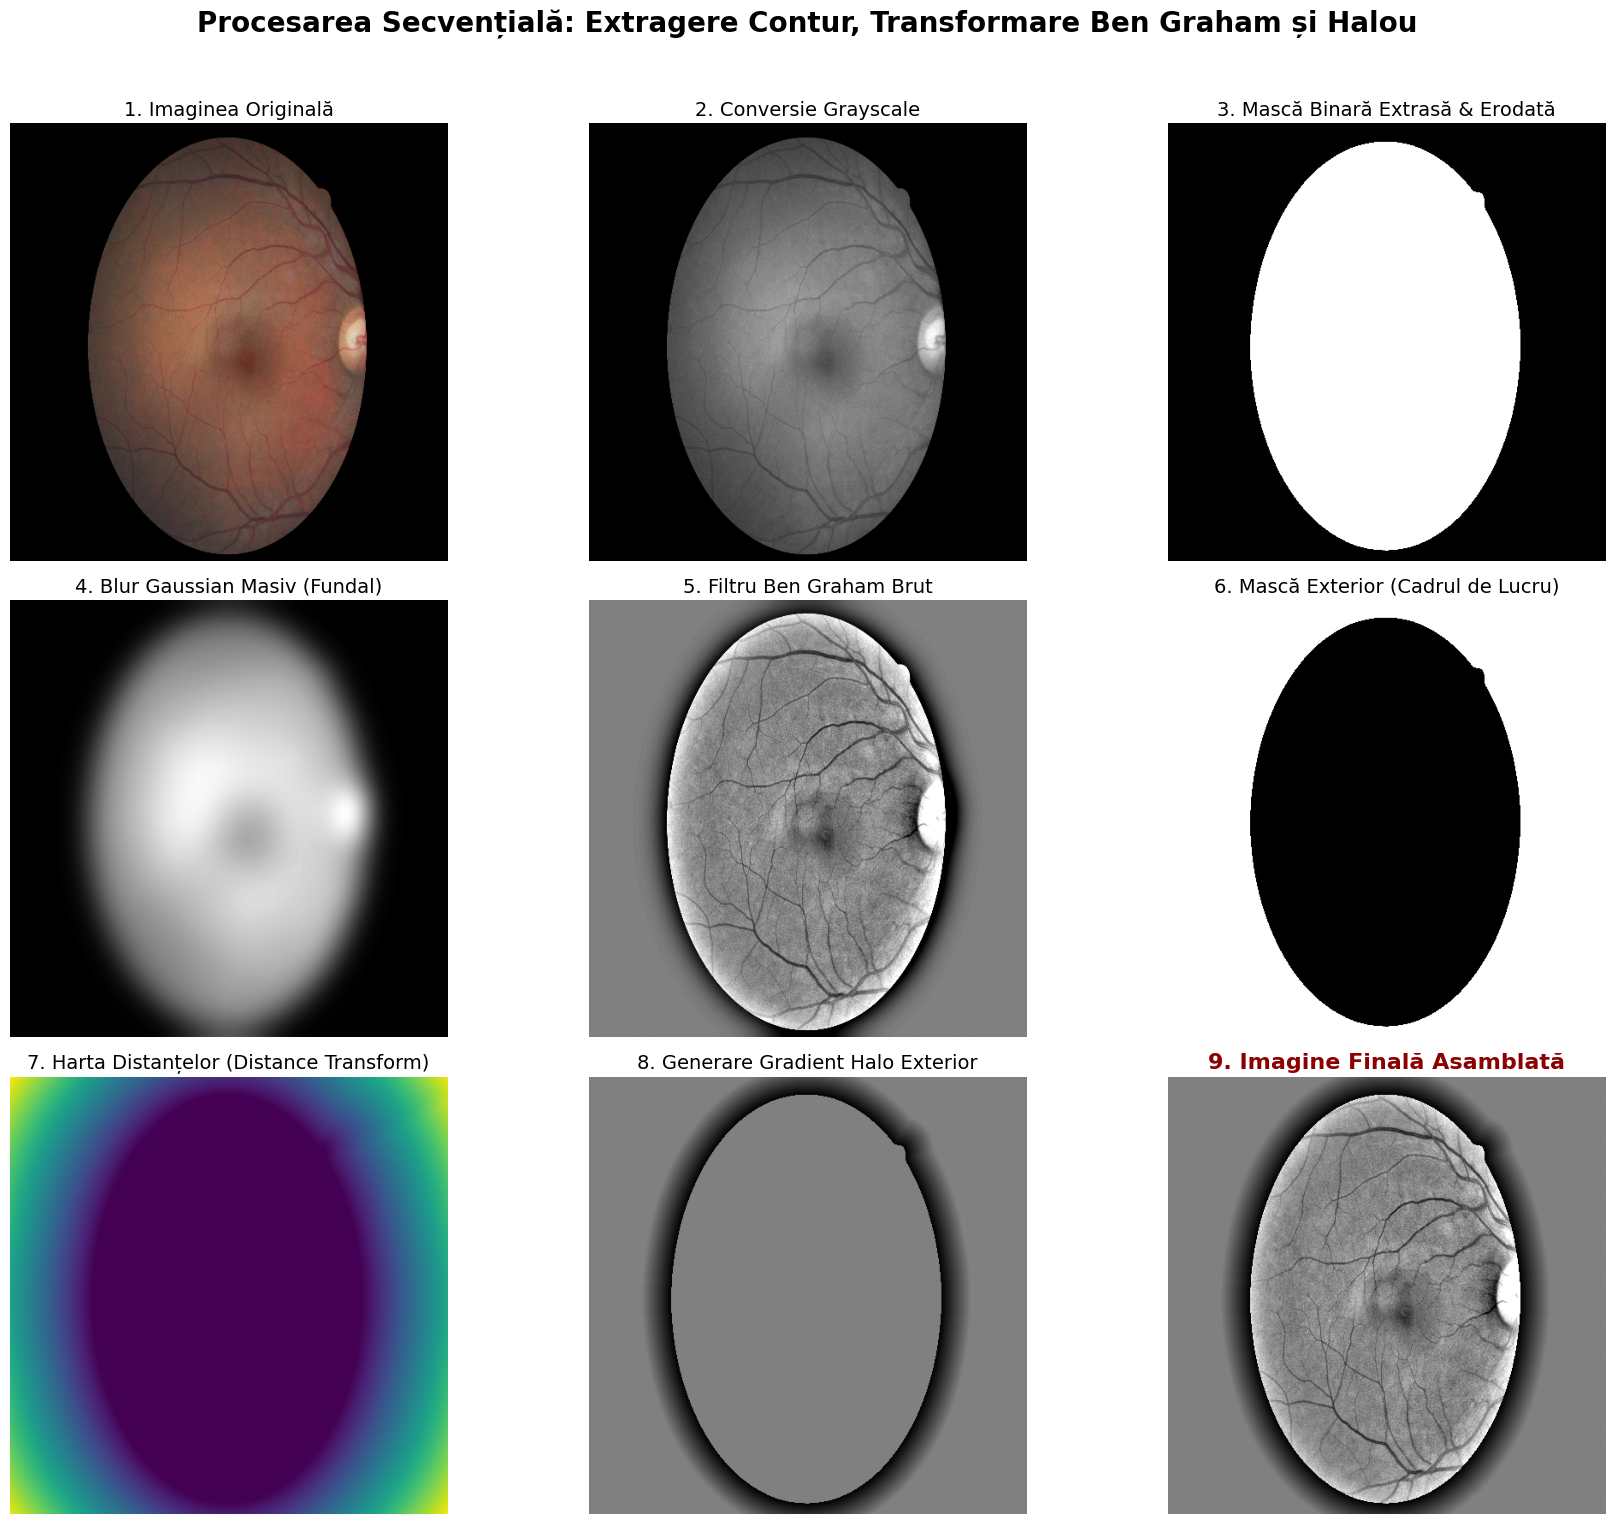
\includegraphics[width=0.95\textwidth]{Figuri/ben_graham_subprocesari.png}
\captionsetup{justification=centering}
\caption{Vizualizarea etapelor de preprocesare Ben Graham: imagine inițială, mască retiniană, estimarea iluminării de fond, filtrare, generarea haloului și imagine finală.}
\label{fig:ben-graham-subprocesari}
\end{figure}

În modelul principal local CUDA, preprocesarea este realizată prin metoda Ben Graham.
Imaginile sunt redimensionate, regiunea retiniană este mascată, iar fundalul este uniformizat
pentru a reduce variațiile de iluminare înainte de utilizarea lor în antrenare.
\bigskip

Preprocesarea Ben Graham a fost aleasă deoarece reduce variațiile globale de iluminare și face
mai vizibile structurile retiniene relevante, fără a introduce o etapă suplimentară de ajustare
locală a contrastului. Totuși, această preprocesare nu a fost presupusă automat ca fiind optimă
pentru toate seturile. Ea a fost testată experimental pe variantele construite, iar rezultatele
sunt discutate în capitolele următoare. Această abordare este importantă deoarece literatura arată
că modelele pot reacționa diferit la schimbări de preprocesare și de domeniu vizual \cite{8_zhang2022multi},
\cite{9_chetoui2020explainable}.

\section{Formarea dataset-urilor EyePACS pentru sistemul principal}

\ \ \ \ Pe lângă variantele EyePACS folosite în experimentele comparative, pentru sistemul principal
în două etape au fost construite două dataset-uri specializate: \texttt{eyepacs\_binar} și
\texttt{eyepacs\_1\_4}. Acestea au fost generate separat deoarece pipeline-ul final nu rezolvă
direct o singură clasificare multiclasă 0--4, ci împarte decizia în două probleme mai controlabile:
detecția bolii și gradarea severității pentru cazurile patologice.
\bigskip

Dataset-ul \texttt{eyepacs\_binar} este construit în notebook-ul
\path{Scripts/EyePACS/create_eyepacs_binar.ipynb}. Scriptul pornește de la fișierul
\texttt{all\_labels.csv} și de la imaginile originale EyePACS, verifică existența fiecărui fișier și
transformă etichetele originale 0--4 într-o problemă binară: clasa 0 devine \textit{sănătos}, iar
clasele 1--4 sunt grupate în clasa \textit{bolnav}. Imaginile sunt preprocesate prin metoda Ben Graham
în momentul copierii în dataset-ul final. Împărțirea urmărește raportul 70\%/15\%/15\%, iar setul de
test este construit explicit 50/50 între imagini sănătoase și imagini patologice, pentru evaluarea
clară a detectorului binar.
\bigskip

După split, subsetul de antrenare al dataset-ului binar este echilibrat prin augmentare offline.
Augmentările sunt aplicate doar în \texttt{train}, astfel încât validarea și testarea să rămână
nealterate. Varianta finală conține 96.664 imagini în train, câte 48.332 pentru fiecare clasă,
13.304 imagini în validare și 13.304 imagini în test. Setul de test conține 6.652 imagini
\textit{sănătos} și 6.652 imagini \textit{bolnav}.
\bigskip

Dataset-ul \texttt{eyepacs\_1\_4} este construit în notebook-ul
\path{Scripts/EyePACS/create_eyepacs_1-4.ipynb}. În această variantă sunt păstrate doar imaginile cu
etichete patologice, adică nivelurile 1, 2, 3 și 4. Scopul său este antrenarea celei de-a doua etape
a sistemului principal, care primește doar cazurile considerate bolnave de detectorul binar și estimează
gradul de severitate. Split-ul inițial este stratificat pe clasele patologice, cu raport 70\% pentru
antrenare, 15\% pentru validare și 15\% pentru test.
\bigskip

Pentru a reduce dezechilibrul puternic dintre stadiile patologice, subsetul de antrenare din
\texttt{eyepacs\_1\_4} este echilibrat prin augmentare offline până la 10.000 imagini pentru fiecare
clasă. Rezultatul final are 40.000 imagini în train, distribuite egal între stadiile 1--4, 3.503
imagini în validare și 3.504 imagini în test. Validarea și testarea păstrează distribuția naturală a
cazurilor patologice, tocmai pentru ca evaluarea modelului de severitate să rămână realistă.
\bigskip

Prin separarea acestor două dataset-uri, sistemul principal poate optimiza diferit cele două obiective.
Primul model este antrenat pentru sensibilitate ridicată în separarea \textit{sănătos}--\textit{bolnav},
iar al doilea model este antrenat doar pe diferențele mai fine dintre stadiile patologice. Această
organizare reduce conflictul dintre clasa majoritară 0 și clasele de boală, problemă frecventă în
clasificarea directă pe scala completă 0--4.

\section{Dataset-urile finale rezultate}

\ \ \ \ În urma acestor pași au rezultat mai multe variante experimentale și două dataset-uri dedicate
sistemului principal. Tabelul
\ref{tab:dataseturi-finale} sintetizează rolul fiecăreia.

\begin{table}[H]
\centering
\caption{Dataset-uri construite și rolul lor în lucrare}
\label{tab:dataseturi-finale}
\scriptsize
\setlength{\tabcolsep}{3pt}
\renewcommand{\arraystretch}{1.25}
\begin{tabularx}{\textwidth}{|>{\raggedright\arraybackslash}p{3.5cm}|>{\raggedright\arraybackslash}p{4.0cm}|>{\raggedright\arraybackslash}X|}
\hline
\textbf{Dataset} & \textbf{Script / sursă} & \textbf{Rol} \\
\hline
\texttt{eyepacs\_split} & \path{split_eyepacs.ipynb} & Split stratificat inițial pentru EyePACS. \\
\hline
\texttt{eyepacs\_cleaned} & \path{clean_eyepacs.ipynb} & Variantă filtrată calitativ. \\
\hline
\texttt{eyepacs\_augmented} & \path{form_eyepacs_augmented.ipynb} & Variantă cu augmentare pentru reducerea dezechilibrului. \\
\hline
\shortstack[l]{\texttt{eyepacs\_augmented}\\\texttt{\_bengraham}} & \shortstack[l]{\path{form_eyepacs_augmented}\\\path{_bengraham.ipynb}} & EyePACS augmentat și preprocesat Ben Graham. \\
\hline
\texttt{eyepacs\_binar} & \path{create_eyepacs_binar.ipynb} & Dataset pentru prima etapă a sistemului principal: clasificare \textit{sănătos}--\textit{bolnav}, cu train echilibrat și test 50/50. \\
\hline
\texttt{eyepacs\_1\_4} & \path{create_eyepacs_1-4.ipynb} & Dataset pentru a doua etapă a sistemului principal: gradarea cazurilor patologice în clasele 1--4, cu train echilibrat la 10.000 imagini/clasă. \\
\hline
\texttt{aptos\_augmented} & \path{form_aptos_augmented.ipynb} & Variantă APTOS construită pentru experimente cu augmentare controlată. \\
\hline
\shortstack[l]{\texttt{aptos\_augmented}\\\texttt{\_bengraham}} & \shortstack[l]{\path{form_aptos_augmented}\\\path{+b_g.ipynb}} & APTOS augmentat și preprocesat Ben Graham, folosit pentru comparații între domenii vizuale. \\
\hline
\shortstack[l]{\texttt{balanced\_aug}\\\texttt{\_cleaned}} & \path{clean_balanced_aug.ipynb} & Variantă curățată din dataset-ul Diabetic\_Balanced\_Aug. \\
\hline
\texttt{balanced\_augmented} & \path{form_balanced_augmented.ipynb} & Variantă echilibrată prin augmentare. \\
\hline
\shortstack[l]{\texttt{balanced\_augmented}\\\texttt{\_bengraham}} & \shortstack[l]{\path{form_balanced_augmented}\\\path{_bengraham.ipynb}} & Variantă augmentată și preprocesată Ben Graham. \\
\hline
\shortstack[l]{\texttt{Diabetic\_Balanced\_Data}\\\texttt{\_grouped\_70\_20\_10}} & \shortstack[l]{\path{grouped_split}\\\path{_diabetic_balanced_data.py}} & Split grupat fără leakage între originale și augmentări. \\
\hline 
\end{tabularx}
\renewcommand{\arraystretch}{1}
\end{table}  

\chapter{Metodologia propusă}

\section{Fluxul general al sistemului}

\ \ \ \ Metodologia propusă urmărește construirea unui flux complet pentru clasificarea automată a retinopatiei
diabetice pe baza imaginilor de fund de ochi. Sistemul pornește de la seturi de date reorganizate
în directoare de antrenare, validare și testare. Pentru experimentele comparative sunt folosite
EyePACS, APTOS și \textit{Diabetic\_Balanced\_Aug}, iar pentru sistemul principal sunt construite
două seturi EyePACS specializate: \texttt{EyePACS\_binar}, pentru separarea imaginilor bolnave de
cele sănătoase, și \texttt{EyePACS\_1\_4}, pentru gradarea severității bolii. Fluxul ajunge la
salvarea unor modele antrenate care pot fi folosite ulterior într-o aplicație de inferență.
Implementarea este realizată în Python, folosind PyTorch pentru
antrenarea rețelelor, Torchvision și \texttt{timm} pentru arhitecturi pre-antrenate, iar scikit-learn, Matplotlib și
Seaborn pentru evaluare și vizualizare.
\bigskip

Fluxul de lucru este împărțit în mai multe componente principale. Fișierul
\texttt{my\_dataset.py} se ocupă de încărcarea imaginilor și de aplicarea transformărilor.
Fișierul \texttt{builder.py} definește modelele, funcțiile de pierdere, modul de calcul al
predicțiilor și optimizatorii. Fișierul \texttt{utils.py} grupează funcțiile auxiliare necesare
pentru rularea experimentelor: crearea directoarelor de rezultate, generarea numelor de fișiere,
calculul metricilor suplimentare, rularea unei epoci de antrenare sau validare, salvarea
graficelor, construirea matricelor de confuzie, a curbelor ROC și a hărților Grad-CAM.
Scriptul \texttt{train.py} integrează aceste componente, rulează antrenarea, validează modelul la
fiecare epocă, salvează cea mai bună variantă și generează graficele de evaluare.
\bigskip

Separarea funcțiilor utilitare într-un fișier dedicat este importantă deoarece menține
\texttt{train.py} concentrat pe fluxul principal al experimentului. În același timp,
\texttt{utils.py} permite reutilizarea acelorași funcții de evaluare și vizualizare pentru mai
multe arhitecturi, surse de date și configurații de antrenare. În experimentele documentate,
QWK este folosită ca metrică principală de salvare a celui mai bun model, iar rezultatele
generate pentru experimente diferite au aceeași structură și pot fi comparate mai ușor.
\bigskip

Problema este formulată ca o clasificare multiclasă în cinci clase, corespunzătoare stadiilor
retinopatiei diabetice. Pentru fiecare imagine, modelul produce un vector de cinci scoruri,
iar clasa finală este obținută prin alegerea valorii maxime în cazul funcțiilor
de pierdere de tip Cross-Entropy și Focal Loss. Pentru varianta ordinală, 
ieșirea continuă a rețelei este interpretată prin praguri de decizie optimizate, 
deoarece clasele au o ordine clinică naturală.
\bigskip

\begin{figure}[H]
    \centering
    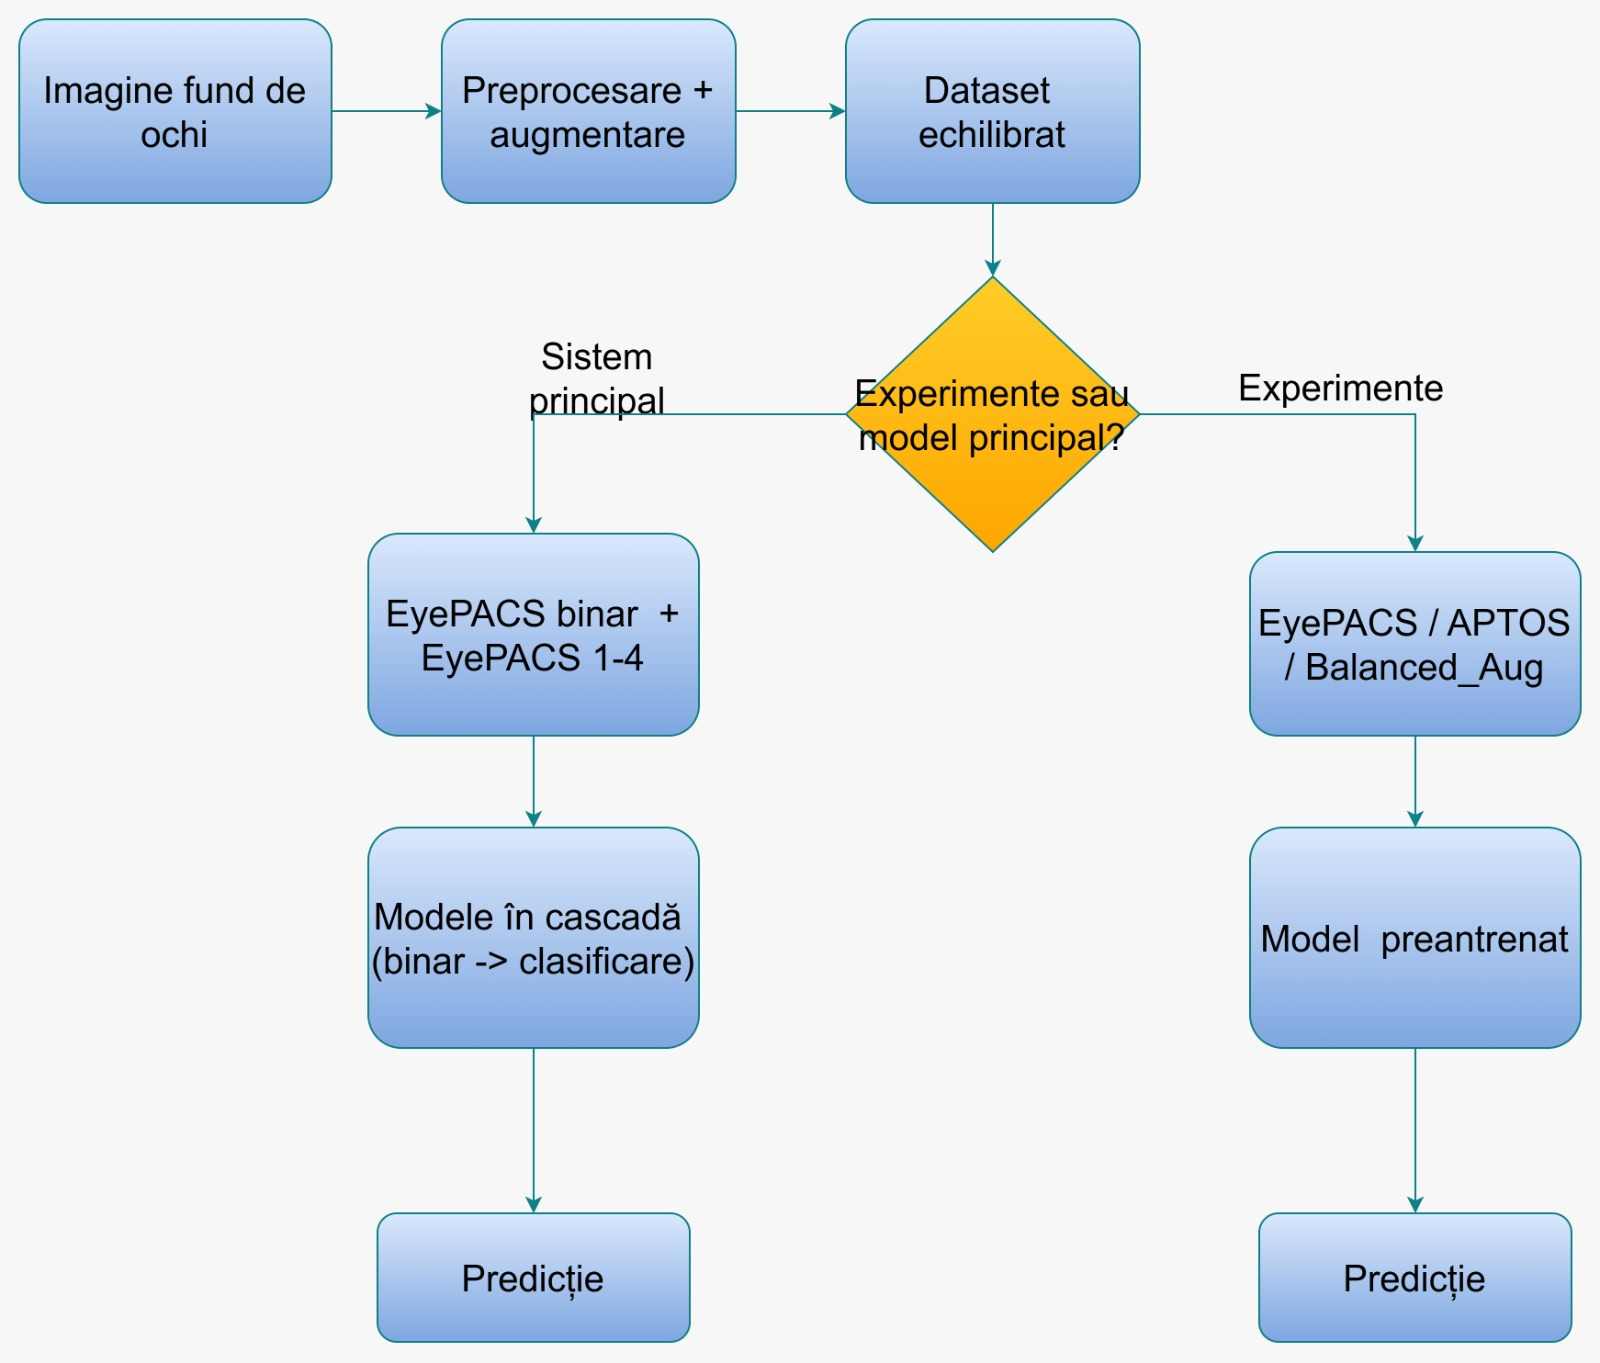
\includegraphics[width=0.98\textwidth]{Figuri/schema_flux_sistem_complet.png}
    \captionsetup{justification=centering}
    \caption{Fluxul general al lucrării, de la imaginea de fund de ochi și preprocesare până la
    ramura de experimente și ramura sistemului principal.}
    \label{fig:schema-flux-sistem-complet}
\end{figure}

\ \ \ \ Figura \ref{fig:schema-flux-sistem-complet} sintetizează organizarea întregului sistem.
Pornind de la imaginea fundus, datele sunt preprocesate și echilibrate, apoi sunt folosite fie pentru
experimente comparative, fie pentru construirea pipeline-ului principal. Ramura experimentală include
evaluarea pe EyePACS, APTOS și \texttt{Diabetic\_Balanced\_Aug}, cu modele preantrenate folosite
pentru compararea arhitecturilor și a strategiilor de antrenare. Ramura principală folosește
\texttt{EyePACS\_binar} pentru decizia bolnav/sănătos și \texttt{EyePACS\_1\_4} pentru gradele de boală,
astfel încât decizia finală să poată fi obținută prin modele în cascadă.
\bigskip 

Pe lângă această formulare multiclasă, soluția principală a lucrării este organizată ca un
pipeline în două etape. Prima etapă tratează problema ca detecție binară și decide dacă imaginea
aparține clasei 0 sau uneia dintre clasele patologice 1--4. A doua etapă este aplicată doar
imaginilor considerate patologice și clasifică severitatea în clasele 1, 2, 3 și 4. Astfel,
decizia finală rămâne exprimată pe scala completă 0--4, dar modelul nu mai trebuie să rezolve
simultan două probleme diferite: separarea imaginilor sănătoase de cele afectate și diferențierea
gradelor de severitate între cazurile bolnave.

\begin{figure}[H]
    \centering
    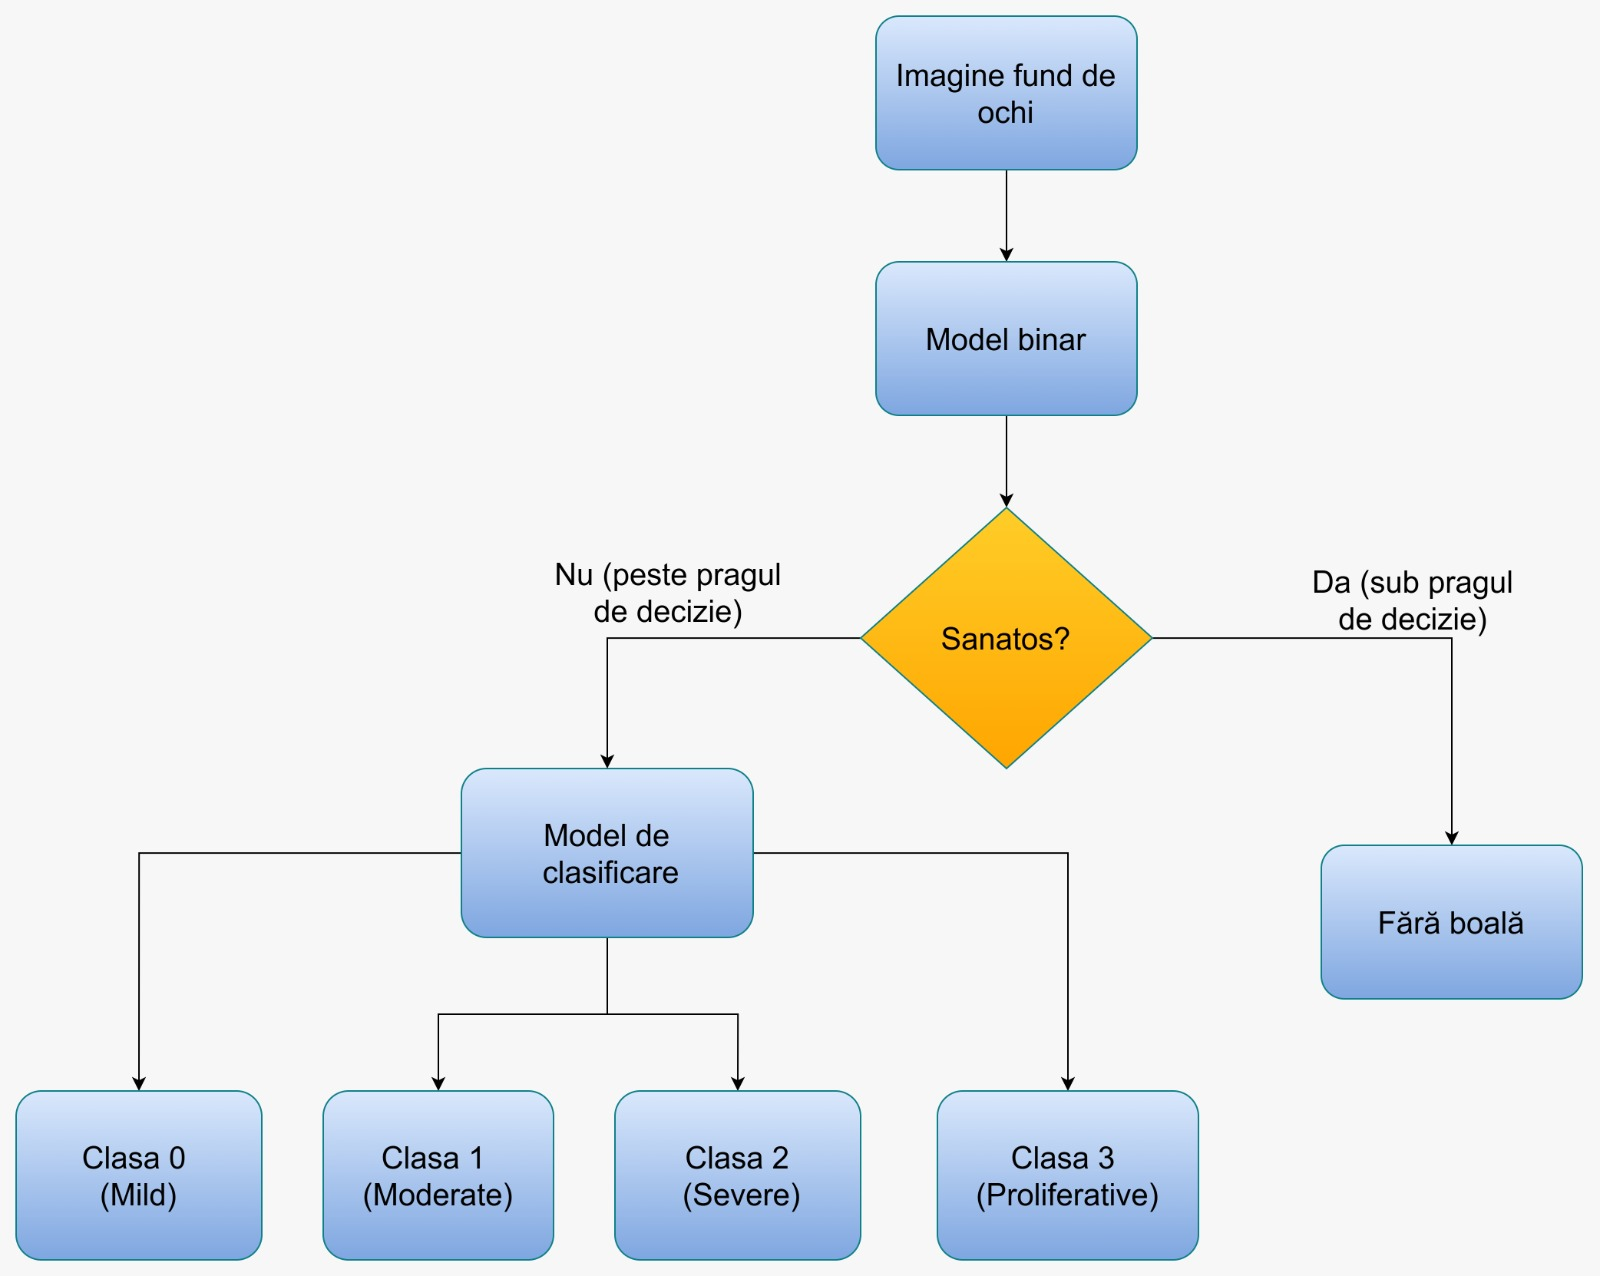
\includegraphics[width=0.88\textwidth]{Figuri/schema_flux_sistem_principal_doua_etape.png}
    \captionsetup{justification=centering}
    \caption{Fluxul sistemului principal în două etape: detector binar pentru separarea imaginilor
    sănătoase de cele patologice, urmat de clasificarea severității pentru cazurile trimise mai departe.}
    \label{fig:schema-flux-sistem-principal-doua-etape}
\end{figure} 

\ \ \ \ Schema din figura \ref{fig:schema-flux-sistem-principal-doua-etape} detaliază ramura principală a
lucrării. Imaginea este evaluată inițial de modelul binar antrenat pe \texttt{EyePACS\_binar}. Dacă
probabilitatea de boală este sub pragul ales pe validare, sistemul returnează direct rezultatul
\textit{fără boală}. Dacă imaginea este considerată patologică, aceasta este transmisă către modelul
de severitate antrenat pe \texttt{EyePACS\_1\_4}, unde scorul continuu este transformat în clasele
1--4 prin praguri optimizate pe validare. Această separare permite tratarea distinctă a obiectivului
de screening și a obiectivului de gradare a bolii.
\bigskip

\section{Modelele analizate}

\ \ \ \ În experimente au fost analizate arhitecturi convoluționale moderne, alese deoarece permit transfer
learning și au fost utilizate frecvent în clasificarea imaginilor medicale \cite{4_pratt2016convolutional}, \cite{10_jabbar2022transfer}.
Implementarea permite construirea modelelor \texttt{resnet50}, \texttt{efficientnet\_b3}, \texttt{inception\_v3} și
\texttt{incres\_v2}. Toate cele patru arhitecturi au fost incluse în implementare, însă în experimentele
comparative accentul a fost pus pe ResNet50 și Inception-ResNet-v2, deoarece oferă două repere
complementare: o arhitectură reziduală robustă și o arhitectură hibridă cu procesare multi-scală.
Pentru sistemul principal în două etape, accentul a fost mutat pe EfficientNet-B3, folosit ca
backbone pentru detectorul binar și pentru modelul de clasificare a severității.
\bigskip

Toate modelele sunt adaptate pentru sarcina experimentală curentă. În experimentele inițiale,
straturile finale, proiectate inițial pentru clasificarea ImageNet, sunt înlocuite sau configurate
astfel încât ieșirea să corespundă celor cinci stadii ale retinopatiei diabetice. În soluția
principală în două etape, același principiu este folosit pentru a construi separat un model cu
ieșire binară pentru detecție și un model de regresie care produce un scor continuu pentru
clasele patologice 1--4.
Folosirea ponderilor pre-antrenate este importantă deoarece permite
reutilizarea unor trăsături vizuale generale, precum muchii, texturi, forme și tranziții de culoare,
care sunt apoi ajustate pentru domeniul medical prin fine-tuning. Această strategie este utilă
în special pentru seturile de date medicale, unde numărul de imagini etichetate este mai
mic decât în colecțiile generale precum ImageNet, iar variațiile de iluminare, contrast și
calitate a achiziției pot influența semnificativ predicția.

\section{Arhitectura ResNet50}

\ \ \ \ ResNet50 este o arhitectură convoluțională bazată pe conexiuni reziduale \cite{21_he2016deep}. Ideea principală
este ca un bloc al rețelei să nu învețe direct o transformare
completă, ci o corecție față de intrarea primită. Această abordare facilitează antrenarea
rețelelor adânci și reduce riscul degradării performanței odată cu creșterea numărului de
straturi. Din acest motiv, ResNet50 este folosită frecvent ca model de referință în
probleme de clasificare medicală: are o capacitate suficient de mare pentru a învăța
trăsături complexe, dar rămâne mai ușor de antrenat și interpretat decât arhitecturile
foarte adânci sau hibride.
\bigskip

În contextul imaginilor de fund de ochi, ResNet50 poate extrage trăsături ierarhice:
primele straturi detectează contururi, variații de culoare și texturi simple, iar straturile
profunde combină aceste informații în structuri mai complexe, precum vase retiniene, zone
de exudate, hemoragii sau regiuni suspecte. În implementarea din \texttt{builder.py}, stratul final
\texttt{fc} este înlocuit cu o secvență formată din \texttt{Dropout(0.5)} și un strat
liniar cu cinci ieșiri. Dropout-ul are rol de regularizare și reduce tendința
de supraînvățare. ResNet50 este astfel folosită atât ca bază de comparație, cât și
ca arhitectură robustă pentru experimentele în care se evaluează influența funcțiilor de
pierdere, a optimizatorilor și a strategiilor de monitorizare.

\section{Arhitectura EfficientNet-B3}

\ \ \ \ EfficientNet-B3 aparține familiei EfficientNet, propusă de Tan și Le \cite{tan2019efficientnet}, în care
scalarea rețelei nu se face independent doar pe adâncime, lățime sau rezoluție, ci
prin \textit{compound scaling}. Această strategie crește simultan cele trei dimensiuni ale modelului
folosind un coeficient comun, astfel încât arhitectura să păstreze un echilibru între
capacitatea de reprezentare și costul computațional. Varianta B3 este relevantă pentru această
lucrare deoarece oferă un compromis între modelele mai mici, care pot pierde detalii fine,
și modelele foarte mari, care necesită mai multă memorie și prezintă risc mai ridicat
de supraînvățare.
\bigskip

Din punct de vedere structural, EfficientNet utilizează blocuri de tip MBConv, inspirate din
convoluțiile separabile pe adâncime și din conexiunile reziduale inversate. Aceste blocuri reduc
numărul de parametri în comparație cu o convoluție standard, păstrând totuși capacitatea de
a extrage trăsături vizuale relevante. Pentru imaginile de fund de ochi, această eficiență
este importantă deoarece leziunile pot fi mici, slab contrastate și distribuite neuniform în
imagine. O arhitectură care procesează intrări la rezoluții mai mari poate păstra mai
bine informația locală, iar mecanismul de scalare al EfficientNet-B3 susține această nevoie fără
a crește excesiv complexitatea modelului.
\bigskip

\begin{figure}[H]
\centering
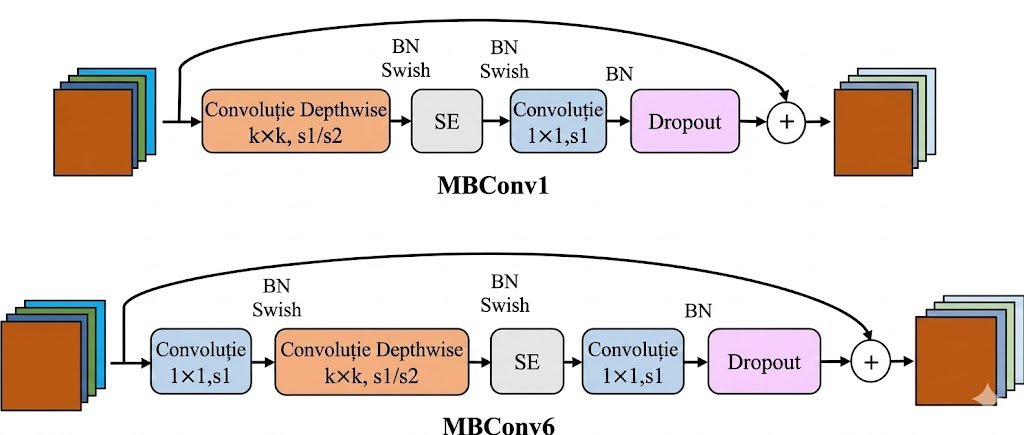
\includegraphics[width=0.95\columnwidth]{Figuri/mbconv_efficientnet_b3.png}
\captionsetup{justification=centering}
\caption{Structura blocurilor MBConv în EfficientNet-B3}
\label{fig:efficientnet-b3-mbconv}
\end{figure}

În implementarea din \texttt{builder.py}, modelul este încărcat prin varianta EfficientNet-B3 din
Torchvision, cu ponderi pre-antrenate atunci când parametrul \texttt{pretrained} este activ.
Clasificatorul final este modificat prin înlocuirea stratului \texttt{classifier[1]} cu o secvență
formată din \texttt{Dropout(0.5)} și un strat liniar cu cinci ieșiri. În cadrul
experimentelor, EfficientNet-B3 oferă o alternativă compactă la ResNet50 și Inception-ResNet-V2, fiind
utilă pentru a verifica dacă o arhitectură optimizată pentru raportul acuratețe--eficiență poate
generaliza bine pe imagini retiniene preprocesate și augmentate. 

\section{Arhitectura InceptionV3}

\ \ \ \ InceptionV3 este o arhitectură construită în jurul modulelor Inception, care procesează aceeași
intrare prin filtre convoluționale de dimensiuni diferite \cite{22_szegedy2016rethinking}. Această strategie permite extragerea
simultană a trăsăturilor locale și a celor cu context spațial mai larg.
Pentru retinopatia diabetică, acest lucru este relevant deoarece semnele patologice pot avea
dimensiuni foarte diferite: microanevrismele sunt mici și discrete, în timp ce hemoragiile
sau exudatele pot ocupa regiuni mai mari. Arhitectura folosește factorizarea convoluțiilor și
module auxiliare pentru a îmbunătăți eficiența și stabilitatea antrenării, fiind una dintre
arhitecturile importante folosite în sisteme de detecție automată a retinopatiei diabetice \cite{3_gulshan2016development}.
\bigskip

În cod, InceptionV3 este încapsulat prin clasa \texttt{InceptionWrapper}. Această clasă rezolvă particularitatea
modelului Torchvision, care în timpul antrenării poate returna și o ieșire auxiliară.
Pentru a păstra aceeași interfață cu funcțiile de pierdere, wrapper-ul returnează doar
predicția principală. Ultimul strat complet conectat este înlocuit cu un strat liniar
cu cinci ieșiri, corespunzătoare claselor 0--4. Prin includerea acestei arhitecturi, metodologia
poate evalua dacă procesarea multi-scală aduce beneficii față de o rețea reziduală standard,
mai ales în situațiile în care semnele clinice apar la scări foarte diferite în aceeași
imagine.

\section{Arhitectura Inception-ResNet-V2}

\ \ \ \ Inception-ResNet-V2 este o arhitectură hibridă care combină modulele Inception cu conexiuni reziduale
\cite{25_szegedy2017inception}.
Din familia Inception preia ideea procesării multi-scală, prin ramuri convoluționale paralele, iar
din familia ResNet preia conexiunile care facilitează propagarea gradientului. Rezultatul este o
rețea profundă, capabilă să învețe reprezentări vizuale bogate fără a pierde stabilitatea
antrenării. În raport cu InceptionV3, arhitectura are o capacitate mai mare și poate
beneficia de stabilitatea conexiunilor reziduale atunci când se realizează fine-tuning pe un set
de date medical.
\bigskip

Această arhitectură este potrivită pentru imaginile retiniene deoarece decizia de severitate poate
depinde atât de leziuni mici, cât și de distribuția globală a modificărilor
patologice. Ramurile Inception pot surprinde structuri la scări diferite, iar conexiunile reziduale
ajută la păstrarea informației utile de-a lungul rețelei. În implementare, modelul este
construit cu biblioteca \texttt{timm}, folosind modelul \texttt{inception\_resnet\_v2} și configurând
direct numărul de clase la cinci. În comparație cu ResNet50, modelul are o capacitate
mai mare, dar în același timp necesită mai multe
resurse de calcul. Din acest motiv, experimentele cu Inception-ResNet-V2 sunt utile pentru
a observa dacă avantajul reprezentărilor mai bogate justifică un cost computațional mai ridicat.

\section{Funcții de pierdere utilizate}

\ \ \ \ Funcția de pierdere definește modul în care modelul este penalizat pentru predicții
greșite. În această lucrare au fost folosite mai multe variante, pentru a compara atât
comportamentul standard în clasificarea multiclasă, cât și strategii mai potrivite pentru clase
dezechilibrate sau ordonate clinic.

\begin{itemize}
  \item \textbf{Cross-Entropy} este funcția de pierdere de bază pentru clasificare multiclasă.
  Aceasta compară distribuția de probabilitate produsă de model cu eticheta reală și oferă
  un punct de referință stabil pentru celelalte experimente. În implementare, această funcție
  poate folosi și \texttt{label\_smoothing}, care distribuie o mică parte din probabilitate către
  celelalte clase și reduce încrederea excesivă a modelului în predicții.

  \item \textbf{Weighted Cross-Entropy} extinde Cross-Entropy prin introducerea unor ponderi pentru clase.
  Această variantă este utilă atunci când anumite clase trebuie penalizate mai puternic, de
  exemplu pentru a reduce tendința modelului de a favoriza clasele mai ușor de învățat.

  \item \textbf{Focal Loss} este implementată prin clasa \texttt{FocalLossMultiClass} și pornește de la
  Cross-Entropy, dar reduce contribuția exemplelor ușoare și acordă mai multă importanță
  exemplelor dificile \cite{20_lin2017focal}. Parametrul \texttt{gamma} controlează cât de puternic este
  accentuată această diferență. În experimentele inițiale a fost analizat intervalul 1.5--2.0,
  iar valoarea 1.6 a fost selectată pentru experimentele extinse deoarece a oferit un
  compromis bun între acuratețe, AUC și distribuția erorilor. La fel ca în cazul Cross-Entropy,
  implementarea permite folosirea parametrului \texttt{label\_smoothing}.

  \item \textbf{Varianta ordinală bazată pe \texttt{BCEWithLogitsLoss}} exploatează faptul că stadiile
  retinopatiei diabetice au o ordine naturală. În loc ca eticheta să fie tratată doar
  ca o clasă independentă, aceasta este transformată într-un vector care descrie nivelurile
  de severitate depășite.

  \item \textbf{BCEWithLogitsLoss pentru detecția binară} este folosită în prima etapă a soluției
  principale, unde modelul trebuie să distingă între imagini sănătoase și imagini cu retinopatie
  diabetică. Această formulare este potrivită deoarece ieșirea modelului este un singur logit,
  interpretat ulterior ca probabilitate de boală.

  \item \textbf{SmoothL1Loss pentru clasificarea 1--4 prin regresie} este folosită în a doua etapă
  a sistemului principal. În această formulare, modelul produce un scor continuu pentru severitatea
  bolii, iar scorul este transformat ulterior în clasele 1--4 prin praguri optimizate pe validare.
  SmoothL1Loss este potrivită aici deoarece combină comportamentul stabil al erorii absolute pentru
  abateri mari cu penalizarea pătratică pentru abateri mici, reducând sensibilitatea la exemple
  izolate dificil de încadrat.
\end{itemize}

\section{Optimizatorul și hiperparametrii de antrenare}

\ \ \ \ Hiperparametrii de antrenare au fost organizați diferit pentru cele două direcții de lucru:
experimentele comparative și sistemul principal în două etape. Experimentele au fost folosite pentru
a compara arhitecturi, seturi de date și funcții de pierdere, în timp ce soluția principală a fost
configurată mai strict, cu două modele \texttt{EfficientNet-B3} antrenate pe dataset-urile dedicate
\texttt{eyepacs\_binar} și \texttt{eyepacs\_1\_4}.

\subsection*{Experimente comparative}

\ \ \ \ Pentru experimente, rulările au fost lansate din notebook-ul
\texttt{experiments.ipynb}, prin apeluri către scriptul de antrenare. Acest cadru a permis modificarea
rapidă a arhitecturii, funcției de pierdere, setului de date și metricii monitorizate. Au fost testate
toate cele patru arhitecturi descrise anterior, respectiv ResNet50, EfficientNet-B3, InceptionV3 și
Inception-ResNet-v2, însă accentul experimental a fost pus pe ResNet50 și Inception-ResNet-v2,
deoarece acestea au fost rulate mai extensiv pe combinațiile finale de date.
\bigskip

\ \ \ \ În aceste rulări au fost comparate \texttt{CrossEntropyLoss},
\texttt{WeightedCrossEntropy} și \texttt{FocalLoss}. Pentru configurațiile finale cu
\texttt{FocalLoss} s-a folosit și \texttt{label\_smoothing} 0.05, cu rolul de a reduce supraîncrederea
modelului și de a evita predicțiile excesiv de rigide pe clasele dominante. În etapa de explorare au
fost testate și valori diferite pentru parametrul \(\gamma\) al Focal Loss, în special în jurul
intervalului 1.5--2.0, pentru a observa cât de mult trebuie accentuate exemplele mai greu de clasificat.
\bigskip

\ \ \ \ Majoritatea configurațiilor comparative recente folosesc \texttt{AdamW}, batch size 32 și
8 workeri pentru încărcarea datelor. Pentru rulările mai vechi sau pentru încercările inițiale au
existat și variante cu Adam sau cu setări implicite ale scriptului, însă configurațiile păstrate pentru
comparațiile finale folosesc în principal \texttt{AdamW}. Acesta este potrivit pentru fine-tuning-ul
modelelor pre-antrenate deoarece separă regularizarea prin \texttt{weight\_decay} de actualizarea
adaptivă a gradientului, ceea ce ajută la controlul supraînvățării fără a destabiliza complet
ponderile deja învățate.
\bigskip
 
\ \ \ \ Pentru rulările comparative finale cu ResNet50 și Inception-ResNet-v2 a fost folosit un
scheduler de tip \texttt{cosine}. Acesta reduce rata de învățare gradual pe parcursul antrenării, fără
scăderi bruște, ceea ce este util în fine-tuning deoarece permite modelului să facă actualizări mai
mari la început și ajustări mai fine spre final. În acest mod, primele epoci pot adapta rapid capul de
clasificare și straturile superioare, iar ultimele epoci stabilizează reprezentările fără a modifica
agresiv ponderile pre-antrenate.
\bigskip

\ \ \ \ Backbone-ul a fost înghețat pentru primele 3 epoci prin
\texttt{freeze\_backbone\_epochs}. Această alegere a fost folosită pentru a antrena inițial doar capul
nou de clasificare, care pornește de la ponderi inițializate aleator. Dacă întregul model ar fi fost
actualizat încă de la început, gradientul produs de un cap încă instabil ar fi putut perturba
caracteristicile deja învățate pe ImageNet. După această etapă, backbone-ul este dezghețat și antrenat
cu o rată de învățare mai mică decât capul, prin \texttt{backbone\_lr\_mult} 0.1. Astfel, straturile
convoluționale pre-antrenate sunt ajustate prudent la imaginile de fund de ochi, în timp ce capul de
clasificare rămâne suficient de flexibil pentru a învăța separarea dintre clase.
\bigskip

\ \ \ \ În plus, s-a folosit \texttt{grad\_clip} 1.0 pentru limitarea normei gradientului. Această
setare previne actualizările foarte mari ale parametrilor, care pot apărea mai ales când se folosesc
dataset-uri diferite, clase dezechilibrate sau funcții de pierdere precum \texttt{FocalLoss}. Pentru
stabilizarea suplimentară a antrenării a fost activată și media mobilă exponențială a ponderilor,
\texttt{ema\_decay} 0.999. EMA păstrează o versiune netezită a parametrilor modelului, reducând
influența oscilațiilor de la o epocă la alta și ajutând la obținerea unui checkpoint mai stabil pe
setul de validare.
\bigskip

\ \ \ \ În funcție de arhitectură și dataset, rulările au fost configurate cu aproximativ 30--50 de
epoci. Pentru comparațiile finale s-a folosit \texttt{early\_stopping\_patience} 15 și \newline
\texttt{early\_stopping\_min\_delta} 0.001. În rulările inițiale au existat și configurații
monitorizate după acuratețe, însă pentru experimentele relevante din documentație modelul a fost
salvat după QWK pe validare, deoarece această metrică respectă caracterul ordinal al claselor de
retinopatie diabetică.
\bigskip

\ \ \ \ Alegerea metricii de monitorizare este importantă deoarece aceasta decide ce checkpoint este
păstrat, nu doar cum este raportată performanța la final. Acuratețea poate fi utilă ca indicator
general, dar în clasificarea retinopatiei diabetice nu surprinde severitatea erorilor: o confuzie între
clasele 1 și 2 este tratată la fel ca o confuzie între clasele 0 și 4. Din acest motiv, pentru
experimentele comparative finale s-a folosit QWK pe setul de validare. QWK măsoară acordul dintre
predicții și etichetele reale, corectând acordul care ar putea apărea întâmplător și penalizând mai
puternic erorile între clase îndepărtate. Pentru o problemă ordinală precum clasificarea gradelor
0--4, această proprietate este mai apropiată de interpretarea clinică a rezultatului decât o simplă
rată de predicții corecte.

\subsection*{Sistemul principal în două etape}

\ \ \ \ Soluția principală nu folosește aceeași configurație generică precum experimentele, ci un
notebook local dedicat, în care hiperparametrii sunt fixați explicit pentru fiecare dintre cele două
modele. Ambele etape folosesc \texttt{EfficientNet-B3}, imagini redimensionate la \(300 \times 300\)
pixeli, batch size 32, 8 workeri și \texttt{Dropout} 0.40 în capul modelului. Alegerea acestei
arhitecturi pentru sistemul principal a fost motivată de raportul bun dintre performanță și costul de
antrenare, dar și de rezoluția nativă de 300 de pixeli, potrivită pentru detaliile din imaginile de
fund de ochi.
\bigskip

\ \ \ \ Prima etapă este detectorul binar sănătos/bolnav. Acesta este antrenat pe
\texttt{eyepacs\_binar} și separă imaginile sănătoase de cele patologice. Funcția de pierdere este
\texttt{BCEWithLogitsLoss}, potrivită pentru o ieșire binară exprimată prin logit. Deoarece dataset-ul
binar a fost construit echilibrat, configurația finală nu activează \texttt{pos\_weight}. Modelul este
antrenat timp de cel mult 50 de epoci, cu \texttt{early\_stopping\_patience} 30.
\bigskip

\ \ \ \ Antrenarea detectorului binar se face în două faze. În primele 10 epoci backbone-ul este
înghețat, iar optimizerul \texttt{AdamW} actualizează doar capul nou al modelului, cu rată de învățare
\(10^{-3}\) și \texttt{weight\_decay} \(10^{-4}\). După această etapă, backbone-ul este dezghețat și
se aplică fine-tuning diferențiat: \(10^{-4}\) pentru backbone și \(3 \cdot 10^{-4}\) pentru capul de
clasificare. Scheduler-ul este \texttt{ReduceLROnPlateau}, cu \texttt{factor} 0.5 și \texttt{patience}
2, aplicat pe AUC-ul de validare. Cel mai bun checkpoint este salvat când AUC-ul de validare se
îmbunătățește cu cel puțin \(10^{-4}\).
\bigskip

\ \ \ \ Pentru detectorul binar, AUC a fost folosit ca metrică principală de monitorizare deoarece
evaluează capacitatea modelului de a separa imaginile sănătoase de cele patologice pe întreg intervalul
de praguri posibile. În această etapă, ieșirea modelului este un scor continuu înainte de aplicarea
pragului final, iar AUC verifică dacă imaginile bolnave tind să primească scoruri mai mari decât cele
sănătoase. Această perspectivă este mai robustă decât acuratețea atunci când pragul de decizie poate fi
ajustat ulterior sau când distribuția setului de validare nu reflectă perfect distribuția reală de
utilizare. Practic, AUC este potrivit pentru prima etapă deoarece obiectivul ei este trierea: modelul
trebuie să separe cât mai bine cazurile normale de cele care trebuie trimise către clasificarea de
severitate. 
\bigskip  

\ \ \ \ Formal, AUC poate fi interpretat ca aria de sub curba ROC:
\[
\mathrm{AUC} = \int_{0}^{1} \mathrm{TPR}(u)\,du,
\]
unde \(u\) reprezintă rata de fals pozitive, iar \(\mathrm{TPR}\) este rata de adevărat pozitive
obținută pentru diferite praguri de decizie. O interpretare echivalentă, mai intuitivă pentru cazul
binar, este:
\[
\mathrm{AUC} = P(s^+ > s^-) + \frac{1}{2}P(s^+ = s^-),
\]
unde \(s^+\) este scorul atribuit unei imagini patologice, iar \(s^-\) este scorul atribuit unei
imagini sănătoase. Astfel, AUC măsoară probabilitatea ca modelul să ordoneze corect o imagine bolnavă
înaintea uneia sănătoase. Un AUC egal cu 0.5 indică un model fără capacitate reală de separare, similar
alegerii aleatoare, iar un AUC apropiat de 1 indică o separare foarte bună între cele două clase.
\bigskip

\ \ \ \ A doua etapă este modelul de severitate 1--4, antrenat doar pe imaginile patologice din
\texttt{eyepacs\_1\_4}. În varianta finală, problema este formulată ca regresie ordinală: modelul
produce un scor continuu, iar acesta este transformat în clasele 1--4 prin praguri optimizate pe setul
de validare. Funcția de pierdere folosită pentru această variantă este \texttt{SmoothL1Loss}. În
notebook există și configurația cu \texttt{CrossEntropyLoss} și \texttt{label\_smoothing} 0.10, însă
soluția principală folosește varianta regresivă deoarece se aliniază mai bine cu ordinea naturală a
gradelor bolii.
\bigskip

\ \ \ \ Modelul 1--4 este antrenat tot în două faze, dar cu backbone-ul înghețat pentru primele 5
epoci din totalul maxim de 50. În faza inițială se antrenează doar capul cu \texttt{AdamW}, rată de
învățare \(10^{-3}\) și \texttt{weight\_decay} \(10^{-4}\). În faza de fine-tuning se folosesc aceleași
rate diferențiate ca în detectorul binar: \(10^{-4}\) pentru backbone și \(3 \cdot 10^{-4}\) pentru
cap. Scheduler-ul este \texttt{ReduceLROnPlateau}, cu \texttt{factor} 0.5 și \texttt{patience} 2,
aplicat pe QWK-ul de validare. Checkpoint-ul final este ales după QWK, cu prag minim de îmbunătățire
\(10^{-4}\) și \texttt{early\_stopping\_patience} 30.
\bigskip

\ \ \ \ Pentru modelul de severitate, QWK este metrica de monitorizare principală deoarece clasele
1--4 reprezintă niveluri ordonate ale aceleiași boli. În acest caz, nu toate erorile au aceeași
semnificație: o predicție de clasă 2 pentru o imagine de clasă 3 este mai acceptabilă decât o predicție
de clasă 1 pentru o imagine de clasă 4. QWK introduce această idee direct în criteriul de selecție a
checkpoint-ului, prin penalizarea pătratică a diferențelor mari dintre clasa reală și clasa prezisă.
De aceea, modelul nu este ales doar pentru că obține multe predicții exacte, ci pentru că păstrează cât
mai bine ordinea clinică a severității. Această alegere este cu atât mai importantă în varianta
regresivă, unde scorul continuu este convertit în clase prin praguri optimizate pe validare.
\bigskip

\ \ \ \ Formula generală pentru QWK este:
\[
\kappa = 1 - \frac{\sum_{i=0}^{K-1}\sum_{j=0}^{K-1} w_{ij} O_{ij}}
{\sum_{i=0}^{K-1}\sum_{j=0}^{K-1} w_{ij} E_{ij}},
\]
unde \(K\) este numărul de clase, \(O_{ij}\) este matricea observată a clasificărilor, adică numărul
de exemple cu eticheta reală \(i\) și predicția \(j\), iar \(E_{ij}\) este matricea acordului așteptat
întâmplător, calculată pe baza distribuțiilor marginale ale etichetelor reale și predicțiilor. Pentru
varianta quadratic weighted, ponderile sunt:
\[
w_{ij} = \frac{(i-j)^2}{(K-1)^2}.
\]
Această pondere este 0 atunci când predicția coincide cu eticheta reală și crește pătratic pe măsură
ce distanța dintre clase devine mai mare. În cazul modelului 1--4, o confuzie între clase vecine are
o penalizare mai mică decât o confuzie între forme ușoare și forme severe. Scorul QWK este apropiat de
1 atunci când acordul dintre predicții și etichete este foarte bun, apropiat de 0 când acordul nu este
mai bun decât cel întâmplător și poate deveni negativ dacă modelul este mai slab decât o atribuire
aleatoare conform distribuțiilor observate.
\bigskip

\ \ \ \ Motivația antrenării în două faze este comună celor două modele principale. Separarea
antrenării capului de fine-tuning-ul backbone-ului reduce riscul ca un cap inițializat aleator să
degradeze rapid reprezentările pre-antrenate. Ratele de învățare diferențiate păstrează stabilitatea
caracteristicilor extrase de \texttt{EfficientNet-B3}, în timp ce capul nou poate învăța mai rapid
distribuția dataset-ului curent. În plus, alegerea metricii monitorizate este specifică fiecărei
etape: AUC pentru detectorul binar, unde contează separarea robustă între sănătos și bolnav, și QWK
pentru clasificarea severității, unde ordinea claselor este esențială. În ambele cazuri, metrica de
monitorizare este folosită atât pentru scheduler, cât și pentru salvarea celui mai bun model, astfel
încât optimizarea să urmărească direct comportamentul dorit al fiecărei ramuri din sistem.

\section{Strategia de evaluare}

\ \ \ \ Evaluarea se realizează în două etape. În timpul antrenării, modelul este monitorizat
pe setul de validare, iar cea mai bună variantă este salvată pe
disc. La final, modelul salvat este reîncărcat și evaluat pe setul de
testare. Pentru experimentele de generalizare între domenii, implementarea permite evaluarea aceluiași model
pe mai multe seturi de test în aceeași rulare, prin argumentul \texttt{test\_sources}.
Astfel, un model antrenat pe date combinate poate fi testat separat pe
APTOS și pe setul Balanced, fără reluarea antrenării. Această separare este necesară
pentru ca testarea să rămână o evaluare cât mai obiectivă a modelului
ales.
\bigskip

Metricile urmărite sunt funcția de pierdere, acuratețea, AUC-ul multiclasă, quadratic weighted
kappa, raportul de clasificare, matricea de confuzie și curbele ROC. AUC-ul este calculat în
regim one-vs-rest și mediat macro, astfel încât fiecare clasă să contribuie egal la scorul final.
\bigskip

Pentru retinopatia diabetică, QWK este relevantă deoarece clasele au
o ordine naturală. O eroare între două clase vecine este mai puțin gravă
decât o eroare între clase îndepărtate, iar această metrică penalizează mai puternic
diferențele mari de severitate. Din acest motiv, experimentele recente folosesc frecvent
QWK ca metrică principală de monitorizare. În plus, scriptul include generarea de hărți
Grad-CAM, utile pentru a observa regiunile imaginii care influențează predicția modelului.

\begin{figure}[H]
\centering
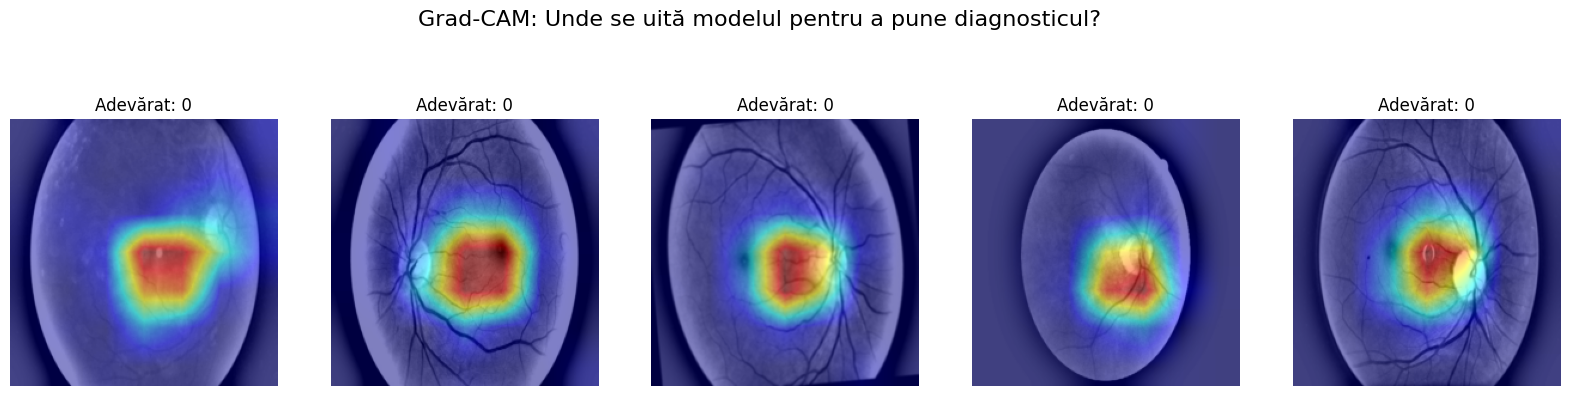
\includegraphics[width=0.95\columnwidth]{Figuri/cam_resnet50.png}
\captionsetup{justification=centering}
\caption{Exemplu de hărți Grad-CAM pentru un model ResNet50 antrenat cu Focal Loss și Adam}
\label{fig:grad-cam-example}
\end{figure}
 
\section{Implementarea procesului de antrenare}

\ \ \ \ Scriptul \texttt{train.py} coordonează întregul proces experimental. După citirea argumentelor, acesta selectează dispozitivul
de calcul disponibil, creează directoarele pentru rezultate și încarcă datele prin clasele
de dataset definite în \texttt{my\_dataset.py}. Implementarea permite folosirea surselor \texttt{balanced}, \texttt{balanced\_aug}, \texttt{aptos},
precum și a combinațiilor \texttt{combined} și \texttt{balanced\_aug\_aptos}. În plus, scriptul poate primi
mai multe directoare de dataset pentru antrenare și le poate trata ca o sursă comună,
concatenată. Astfel, un experiment poate fi rulat pe imagini provenite din mai multe distribuții,
fără a crea manual un nou director intermediar. În mod similar, testarea poate fi făcută pe
mai multe seturi, fiecare păstrat ca sursă separată de evaluare. Fiecare dataset este transmis
către un \texttt{DataLoader}, cu \texttt{shuffle=True} pentru antrenare și \texttt{shuffle=False}
pentru validare și testare.
\bigskip

Pentru fiecare epocă, modelul trece printr-o fază de antrenare și una de
validare. În faza de antrenare se calculează gradientul și se actualizează parametrii,
iar în faza de validare calculele sunt realizate fără gradient. Dacă metrica
de selecție se îmbunătățește, ponderile sunt salvate într-un fișier \texttt{.pth}. La final,
scriptul generează graficele de istoric, matricea de confuzie, curbele ROC și, atunci
când este posibil, imaginile Grad-CAM. În cazul evaluării pe mai multe surse
de test, fiecare set primește fișiere separate, marcate în nume prin sufixe
precum \texttt{test\_aptos}, \texttt{test\_balanced} sau \texttt{test\_balanced\_aug}.
\bigskip

Un avantaj important al scriptului este flexibilitatea oferită prin argumentele din linia de
comandă. Fără modificarea codului sursă, se poate selecta arhitectura, funcția de pierdere,
optimizatorul, numărul de epoci, dimensiunea batch-ului, rata de învățare, dimensiunea imaginilor,
ponderile claselor, valoarea \texttt{gamma} pentru Focal Loss și metrica folosită pentru salvarea
celui mai bun model. În plus, scriptul permite activarea sau dezactivarea unor tehnici precum
\texttt{amp}, \texttt{grad\_clip}, \texttt{ema\_decay},
\texttt{model\_dropout}, \texttt{freeze\_backbone\_epochs}, \texttt{backbone\_lr\_mult} și
\texttt{early\_stopping\_patience}. Această organizare a fost utilă în experimentele exploratorii,
deoarece aceeași implementare putea fi rulată rapid în configurații diferite.
\bigskip

Flexibilitatea este prezentă și la nivelul dataset-urilor. Argumentele importante din
\texttt{train.py} sunt:

\begin{itemize}
  \item \textbf{\texttt{--train\_dataset\_roots}} primește unul sau mai multe directoare folosite pentru antrenare și validare. Dacă sunt transmise mai multe căi, seturile sunt concatenate logic în timpul încărcării datelor.
  \item \textbf{\texttt{--train\_dataset\_names}} permite atribuirea unor nume clare surselor de antrenare, astfel încât experimentul și fișierele rezultate să poată fi identificate ușor.
  \item \textbf{\texttt{--test\_dataset\_roots}} primește unul sau mai multe directoare folosite pentru testarea finală. Rezultatele sunt raportate separat pentru fiecare sursă de test.
  \item \textbf{\texttt{--test\_dataset\_names}} definește numele surselor de test, folosite apoi în sufixele fișierelor, de exemplu \texttt{test\_aptos} sau \texttt{test\_balanced}.
  \item \textbf{\texttt{--train\_augment}} controlează augmentările online, prin valorile \texttt{basic} și \texttt{none}. Această opțiune este utilă atunci când dataset-ul conține deja augmentări sau imagini preprocesate offline.
  \item \textbf{\texttt{--model}, \texttt{--loss\_name}, \texttt{--optimizer}} selectează arhitectura, funcția de pierdere și optimizatorul, permițând compararea rapidă a configurațiilor experimentale.
  \item \textbf{\texttt{--monitor\_metric}} stabilește criteriul după care este salvat cel mai bun model; în experimentele documentate a fost folosit QWK.
  \item \textbf{\texttt{--scheduler}, \texttt{--amp}, \texttt{--grad\_clip} și \texttt{--ema\_decay}} activează tehnici suplimentare pentru stabilizarea antrenării și evaluării.
\end{itemize}
\bigskip

Astfel, același model poate fi antrenat pe date combinate și testat separat pe APTOS, Balanced
sau Balanced Aug, iar graficele rezultate sunt salvate cu nume care reflectă sursa de antrenare
și sursa de testare. Această organizare a fost utilă pentru experimentele de generalizare între
dataset-uri, deoarece a permis compararea comportamentului modelului pe distribuții diferite în
aceeași rulare experimentală.
\bigskip

Pentru seturile care conțin deja imagini augmentate sau preprocesate, scriptul permite
dezactivarea augmentărilor online prin \texttt{train\_augment=none}. Această opțiune evită aplicarea dublă
a augmentărilor în experimentele recente, păstrând în același timp comportamentul vechi prin
valoarea implicită \texttt{train\_augment=basic}.

\chapter{Rezultate experimentale}

\ \ \ \ Înainte de prezentarea experimentelor principale, capitolul pornește de la rezultatele preliminare
obținute pe setul \texttt{Diabetic\_Balanced\_Data}. Această ordine este utilă deoarece comparațiile
între funcțiile de pierdere și arhitecturi au fost realizate inițial pe un set public care părea potrivit
pentru experimente controlate, dar care a evidențiat ulterior o problemă importantă de \textit{data
leakage}. Astfel, primele secțiuni au rolul de a explica de ce scorurile foarte ridicate trebuie
interpretate cu prudență și de ce a fost necesară reorganizarea datelor înainte de experimentele finale.
\bigskip

După această analiză de context, capitolul continuă cu configurația experimentală folosită pentru
experimentele proprii: comparația dintre APTOS, EyePACS și Balanced\_Aug în variantele baseline,
augmentate și augmentate + preprocesate. În acest fel, rezultatele principale sunt prezentate după ce
au fost clarificate limitele dataset-urilor inițiale și ale protocoalelor afectate de scurgeri de
informație.
\bigskip

\section{Compararea funcțiilor de pierdere pe Diabetic\_Balanced\_Data}

\ \ \ \ Înainte de interpretarea comparațiilor din această secțiune, trebuie menționat explicit că
varianta publică a setului \texttt{Diabetic\_Balanced\_Data} conține \textit{data leakage}, deoarece
augmentări ale aceleiași imagini pot ajunge în subseturi diferite. Din acest motiv, valorile absolute
obținute pe acest set trebuie privite cu prudență și nu trebuie confundate cu o estimare finală a
generalizării. Totuși, setul rămâne util pentru comparații experimentale între funcții de pierdere și
arhitecturi, deoarece toate configurațiile sunt rulate în aceleași condiții, pe aceeași distribuție și
cu același protocol de evaluare.
\bigskip

Figura \ref{fig:cap6-dbd-lossuri-resnet50} sintetizează istoricul funcției de pierdere pentru patru
configurații ResNet50: \textit{focal loss} cu Adam, \textit{cross-entropy} cu Adam,
\textit{weighted cross-entropy} cu AdamW și \textit{focal loss} cu AdamW. Scopul graficului nu este
alegerea unui model final pe baza acestui dataset, ci observarea comportamentului relativ al
funcțiilor de pierdere în timpul antrenării.
\bigskip

Se observă că toate configurațiile învață rapid pe setul de antrenare, însă diferența dintre curba de
antrenare și cea de validare rămâne importantă pentru interpretare. \textit{Cross-entropy} simplu este
o alegere stabilă ca punct de plecare, dar poate favoriza exemplele ușor de clasificat. Varianta
ponderată nu aduce un avantaj clar în acest context, deoarece setul este deja echilibrat artificial,
iar ponderarea suplimentară nu rezolvă principala problemă a datelor. În schimb, \textit{focal loss}
este mai potrivită pentru continuarea experimentelor deoarece pune accent pe exemplele dificile și pe
confuziile care apar între clasele apropiate.
 
\begin{figure}[H]
    \centering
    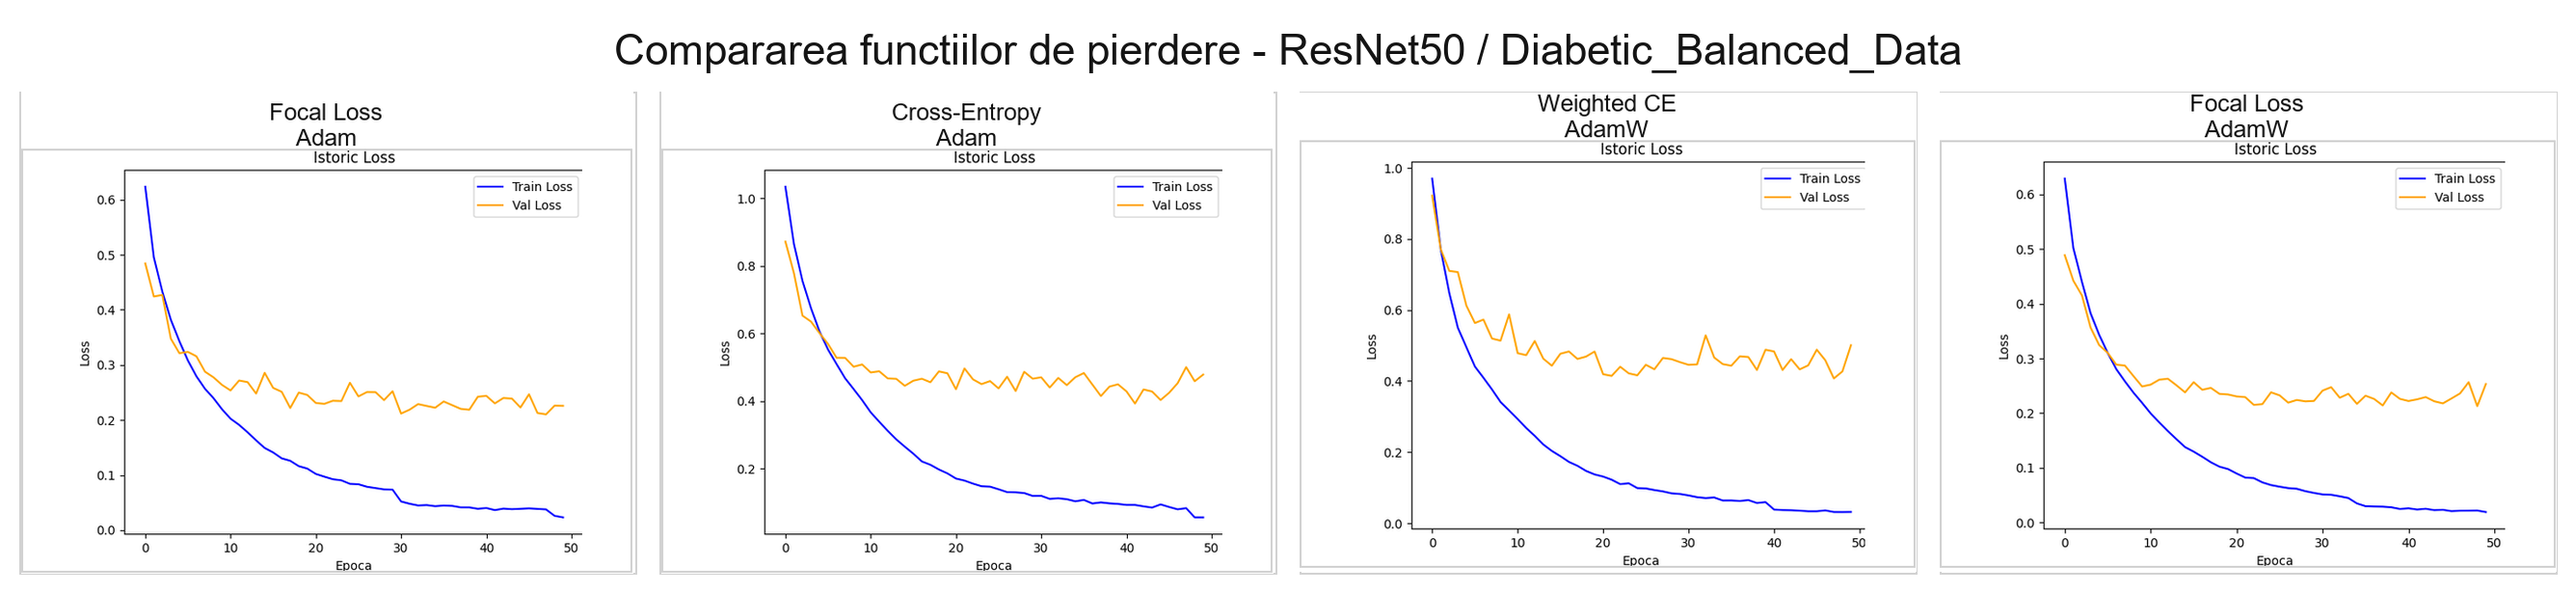
\includegraphics[width=0.98\textwidth]{Figuri/cap6_dbd_lossuri_resnet50.png}
    \captionsetup{justification=centering}
    \caption{Comparația istoricului loss-ului pentru ResNet50 pe \texttt{Diabetic\_Balanced\_Data}.}
    \label{fig:cap6-dbd-lossuri-resnet50}
\end{figure}

\section{Compararea arhitecturilor pe Diabetic\_Balanced\_Data}

\ \ \ \ Pentru comparația arhitecturilor au fost analizate matricile de confuzie absolute pentru
ResNet50, InceptionV3, InceptionResNet-v2 și EfficientNet-B3, în configurații rulate pe același set
\texttt{Diabetic\_Balanced\_Data}. Figura \ref{fig:cap6-dbd-matrici-arhitecturi} arată nu doar câte
imagini sunt clasificate corect, ci și direcția erorilor dintre clase.
\bigskip

Rezultatele sunt apropiate la nivel global, majoritatea configurațiilor obținând valori în jurul
intervalului 0,88--0,90 pentru acuratețe. De aceea, interpretarea relevantă nu este doar
care model are scorul maxim, ci unde apar confuziile. Clasele 3 și 4 sunt recunoscute bine de toate
arhitecturile, ceea ce indică faptul că formele severe au trăsături vizuale mai ușor de separat. În
schimb, clasele 0, 1 și 2 concentrează cele mai importante erori, deoarece diferențele dintre absența
bolii, formele ușoare și formele moderate sunt mai subtile.
\bigskip 

EfficientNet-B3 are comportamentul cel mai echilibrat în aceste teste, cu aproximativ 0,90 acuratețe,
dar diferența față de celelalte arhitecturi nu este suficientă pentru a elimina complet
ResNet50 din analiză. ResNet50 rămâne un baseline robust, mai simplu de antrenat și util pentru
comparațiile dintre preprocesări, augmentări și funcții de pierdere. InceptionV3 și InceptionResNet-v2
confirmă aceeași tendință generală: arhitectura influențează distribuția erorilor, însă calitatea
datelor și protocolul de împărțire rămân decisive.

\begin{figure}[H]
    \centering
    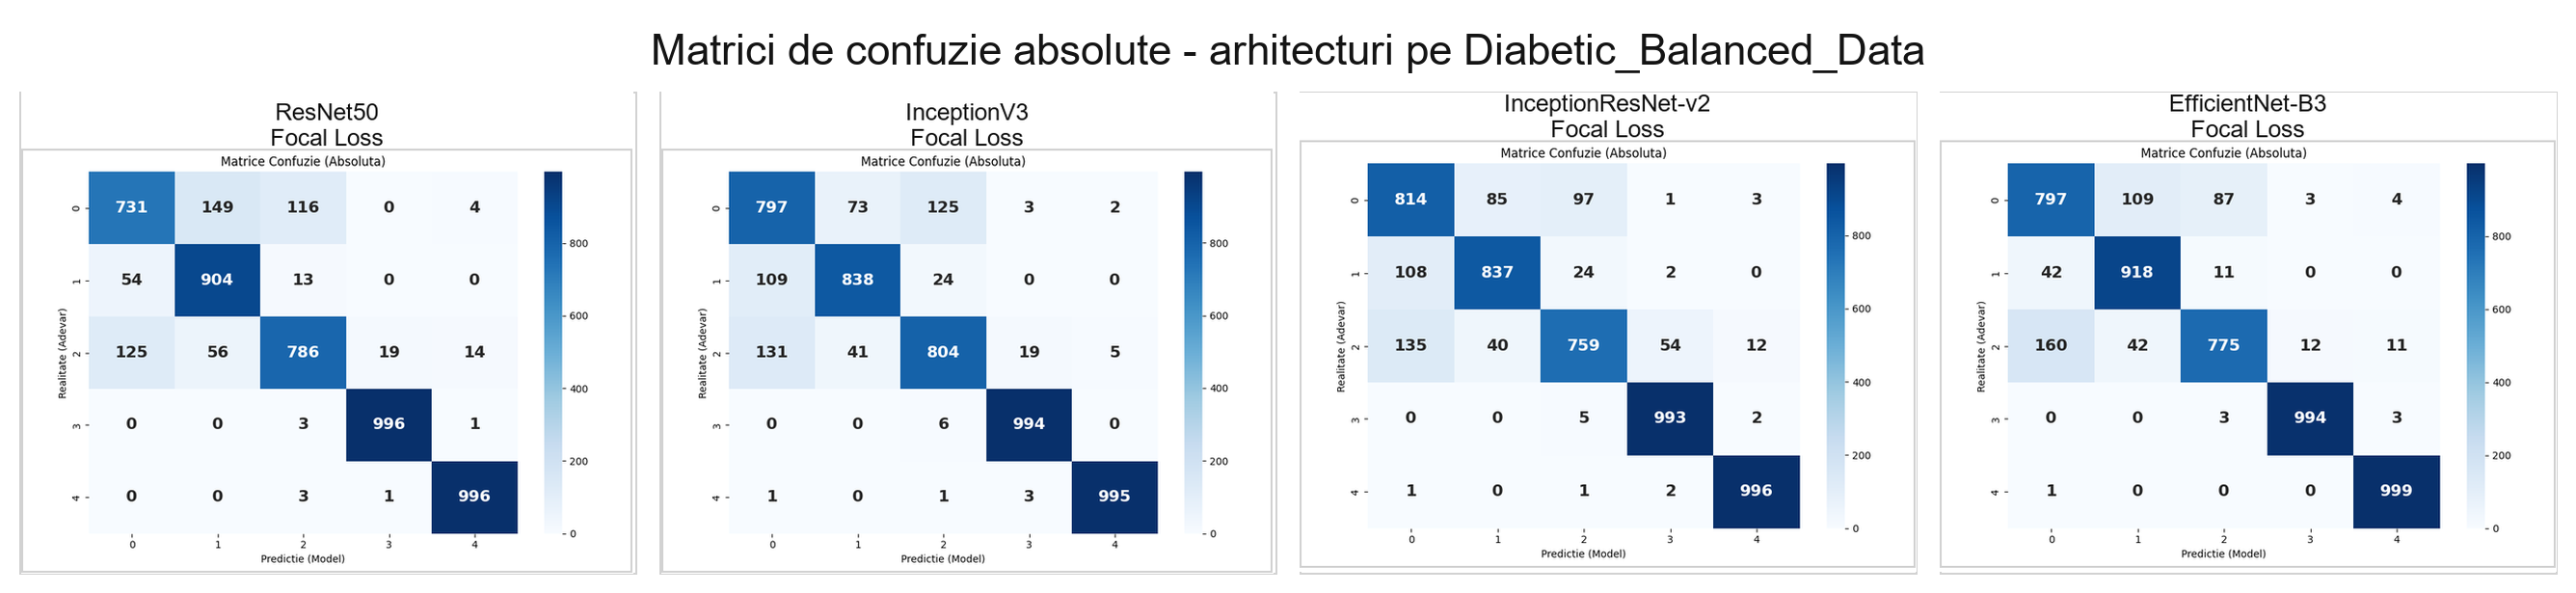
\includegraphics[width=0.98\textwidth]{Figuri/cap6_dbd_matrici_arhitecturi_absolute.png}
    \captionsetup{justification=centering}
    \caption{Matrici de confuzie pentru arhitecturile comparate pe \texttt{Diabetic\_Balanced\_Data}.}
    \label{fig:cap6-dbd-matrici-arhitecturi}
\end{figure}

\section{Analiza data leakage în APTOS și Diabetic\_Balanced\_Data}

\ \ \ \ O etapă separată a analizei a fost dedicată verificării riscului de \textit{data leakage}.
Această verificare a devenit necesară după examinarea setului
\texttt{Diabetic\_Balanced\_Data}, unde imaginile originale și augmentările derivate din aceeași
imagine puteau ajunge în subseturi diferite. Într-un astfel de scenariu, modelul nu mai este evaluat
pe imagini complet independente, ci poate întâlni în validare sau testare variante foarte apropiate
de exemplele văzute la antrenare. Rezultatul este o estimare artificial optimistă a performanței.
\bigskip

Importanța verificării este cu atât mai mare cu cât setul \texttt{Diabetic\_Balanced\_Data} este
disponibil public \cite{24_kaggle_diabetic_balanced} și apare inclusiv în articole de tip review
despre dataset-uri fundus utilizate pentru retinopatie diabetică
\cite{krzywicki2023fundus_review}. Prezența într-o sinteză bibliografică nu garantează însă că
organizarea locală a fișierelor este potrivită pentru un protocol experimental fără scurgeri de
informație. Din acest motiv, ultimele experimente din notebook-ul \texttt{experiments.ipynb}, secțiunea
\textit{Experimente APTOS data-leakage + Balanced\_Data fără data-leakage}, au fost folosite ca
experimente de control.
\bigskip

Primul a fost realizat pe APTOS, deoarece pentru acest set se putea construi direct o
comparație între două fluxuri. În varianta incorectă, augmentarea a fost aplicată înainte de
împărțirea în train, validare și test, ceea ce permite ca transformări ale aceleiași imagini să apară
în subseturi diferite. În varianta corectă, împărțirea a fost realizată înainte de augmentare, iar
augmentările au rămas în subsetul imaginii originale. Diferența dintre rezultate este puternică:
fluxul \textit{augment -\textgreater{} split} obține o acuratețe de 96,20\%, AUC de 0,9982 și QWK de 0,9813,
în timp ce fluxul \textit{split -\textgreater{} augment} coboară la o acuratețe de 82,02\%
și AUC de 0,9170. Această diferență arată că performanța foarte ridicată nu provenea doar din
capacitatea modelului, ci și din contaminarea dintre subseturi.
 
\begin{figure}[H]
    \centering
    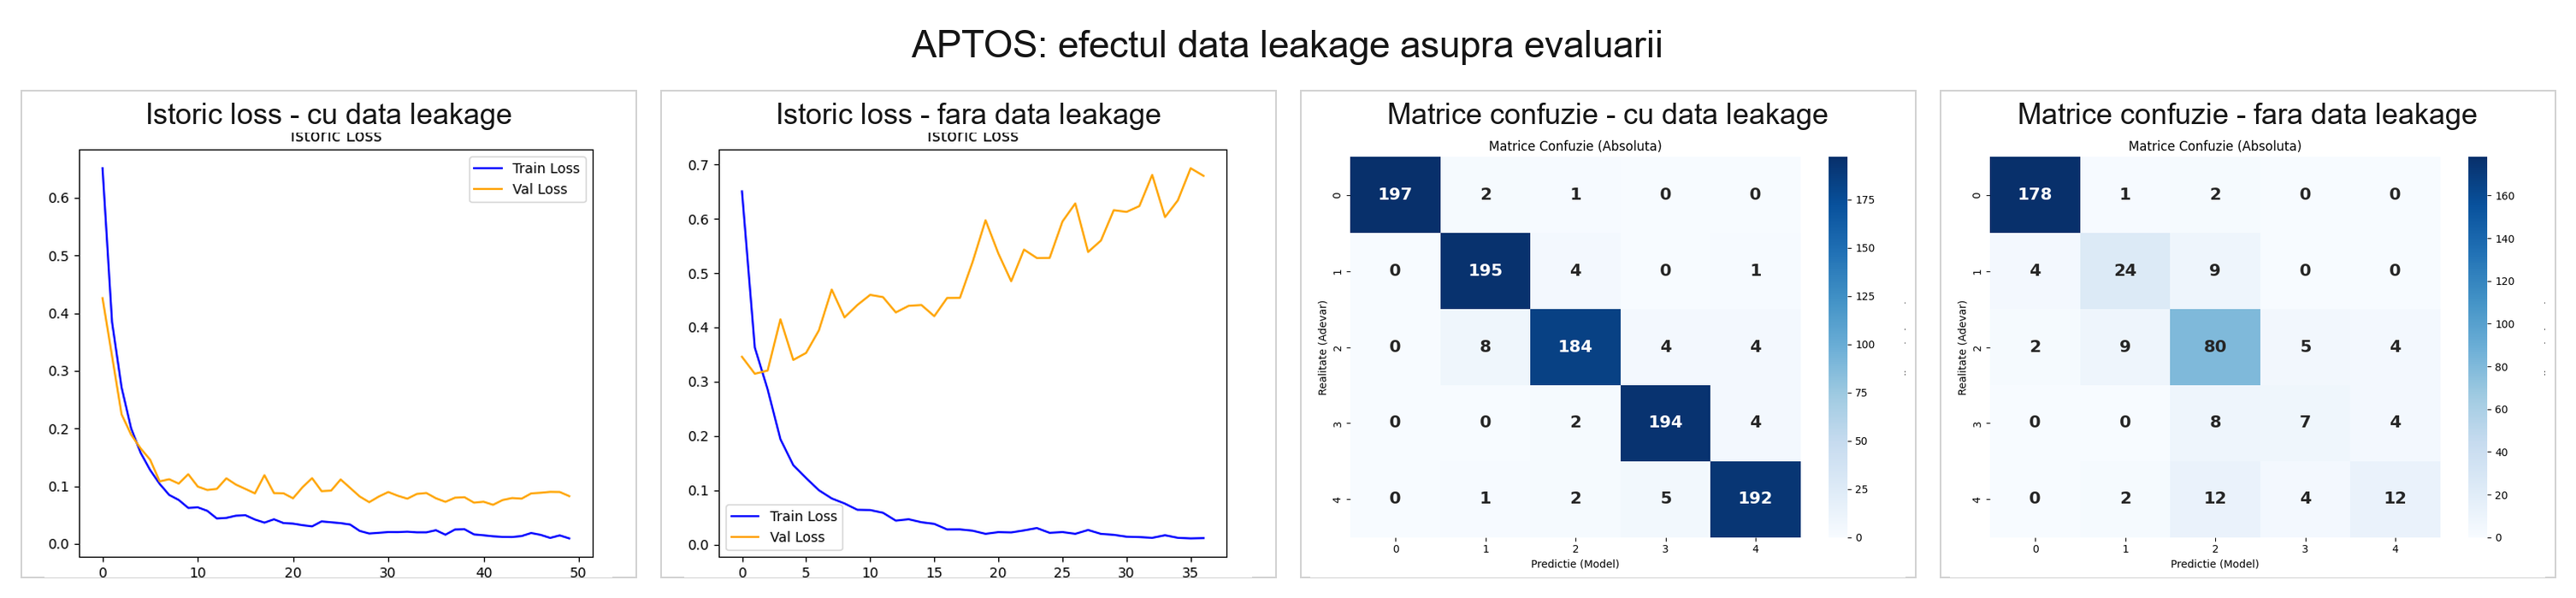
\includegraphics[width=0.98\textwidth]{Figuri/cap6_data_leakage_aptos_comparison.png}
    \captionsetup{justification=centering}
    \caption{Comparație APTOS între fluxul cu \textit{data leakage} și fluxul corect fără \textit{data leakage}: istoricul funcției de pierdere și matricea de confuzie absolută pentru fiecare variantă.}
    \label{fig:cap6-data-leakage-aptos}
\end{figure}

Al doilea control a urmărit direct setul \texttt{Diabetic\_Balanced\_Data}. În varianta distribuită
public, rezultatele sunt ridicate: acuratețe de 88,77\%, AUC de 0,9825 și QWK de 0,9297.
După reorganizarea setului printr-un split grupat, în care imaginea originală și toate
augmentările asociate rămân în același subset, performanța scade la o acuratețe de 60,47\%, AUC de
0,8878 și QWK de 0,7641. Scăderea nu trebuie interpretată ca o degradare a
metodei, ci ca o corectare a protocolului de evaluare: noul rezultat reflectă mai realist capacitatea
modelului de a generaliza pe imagini independente.

\begin{figure}[H]
    \centering
    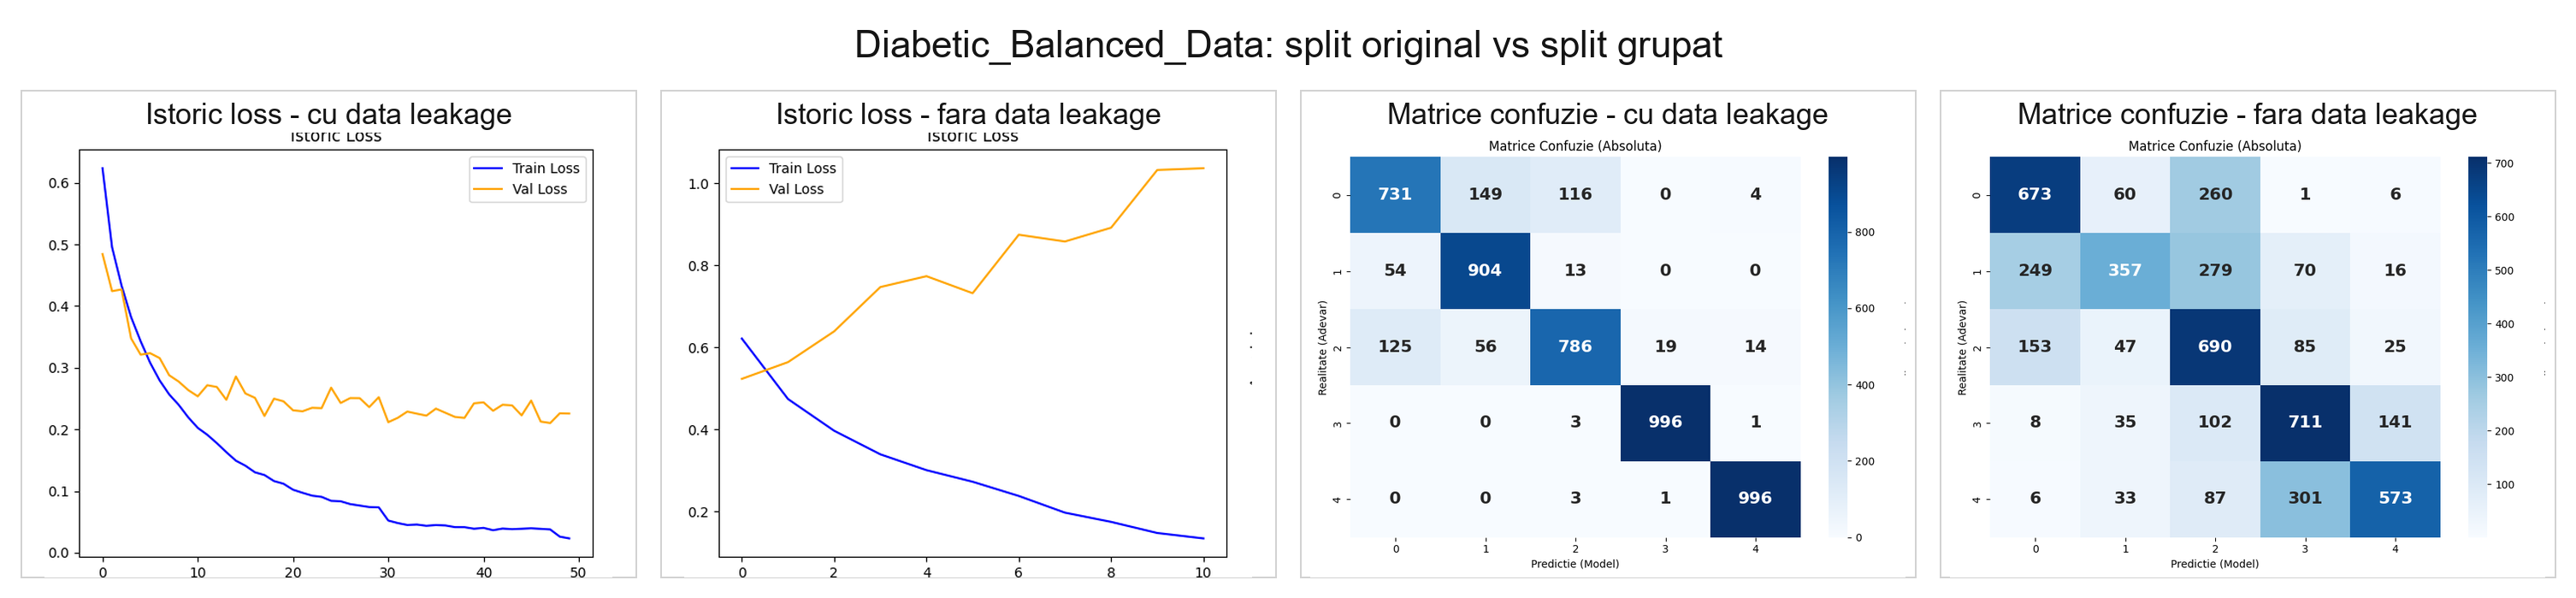
\includegraphics[width=0.98\textwidth]{Figuri/cap6_data_leakage_balanced_comparison.png}
    \captionsetup{justification=centering}
    \caption{Comparație pentru \texttt{Diabetic\_Balanced\_Data} între varianta publică afectată de \textit{data leakage} și varianta rearanjată prin split grupat: istoricul funcției de pierdere și matricea de confuzie absolută pentru fiecare variantă.}
    \label{fig:cap6-data-leakage-balanced}
\end{figure}

După eliminarea scurgerii de informație, matricele de confuzie devin și ele
mai realiste. În varianta cu \textit{data leakage}, diagonala principală este mult mai puternică deoarece modelul
poate recunoaște imagini foarte asemănătoare cu cele văzute în antrenare. În varianta cu split grupat,
confuziile cresc, însă acestea reflectă mai bine dificultatea reală a problemei: modelul trebuie să
generalizeze pe imagini independente, nu pe transformări apropiate ale acelorași funduri de ochi.
\bigskip

Cele mai multe erori apar între clase care sunt apropiate clinic sau vizual. 
\newline
În \texttt{Diabetic\_Balanced\_Data} reorganizat, clasa 1 este confundată frecvent cu clasele 0 și 2,
deoarece semnele de retinopatie ușoară sunt subtile și pot fi apropiate fie de imagini normale, fie de
forme moderate. Clasa 2 este confundată atât cu 0, cât și cu 3, ceea ce indică dificultatea delimitării
stadiului moderat atunci când leziunile sunt parțiale, mici sau afectate de calitatea imaginii. Pentru
clasele severe, se observă confuzii între 3 și 4, deoarece ambele pot conține leziuni avansate, iar
diferența dintre retinopatie severă și proliferativă nu este întotdeauna evidentă doar din imaginea
globală. Aceste confuzii sunt de așteptat într-un protocol corect și sunt mai utile pentru analiză
decât o matrice aproape perfectă obținută prin contaminarea subseturilor.
\bigskip

Aceste experimente justifică folosirea variantei reorganizate cu split grupat și a scriptului
\path{Scripts/DIabetic_Balanced_Data/grouped_split_diabetic_balanced_data.py}. Ele arată că, în
clasificarea retinopatiei diabetice, protocolul de împărțire a datelor este la fel de important ca
arhitectura sau funcția de pierdere. În plus, ele explică de ce rezultatele obținute pe seturi care
conțin augmentări preexistente trebuie interpretate cu prudență: o acuratețe mare poate semnala un
model bun, dar poate semnala și faptul că separarea train--validare--test nu a fost suficient de
strictă sau dezechilibru între clase.

\section{Configurația experimentală}

\ \ \ \ Capitolul de rezultate este actualizat pe baza experimentelor rulate în notebook-ul
\newline \texttt{experiments.ipynb}. Spre deosebire de varianta inițială, care compara în principal
arhitecturi și configurații izolate, analiza de față urmărește efectul etapelor de lucru asupra
seturilor de date: varianta de bază, varianta cu augmentări și varianta în care augmentările sunt
combinate cu preprocesări de tip Ben Graham. Pentru a păstra comparația coerentă, rezultatele sunt
prezentate sub forma unei matrici experimentale cu trei coloane și trei linii.
\bigskip

Coloanele corespund surselor de date analizate:
\begin{itemize}
    \item \textbf{APTOS} -- setul APTOS 2019 reorganizat local și extins cu variante augmentate și preprocesate;
    \item \textbf{EyePACS} -- setul EyePACS procesat local, folosit pentru a observa comportamentul pe o sursă mare și variabilă;
    \item \textbf{Balanced\_Aug} -- setul derivat din Diabetic\_Balanced\_Aug, utilizat pentru a analiza efectul echilibrării și al augmentărilor.
\end{itemize}

Liniile urmăresc gradul de intervenție asupra datelor:
\begin{itemize}
    \item \textbf{Baseline} -- imaginile reorganizate și împărțite în partiții de antrenare, validare și testare;
    \item \textbf{Augmentări} -- imaginile extinse prin transformări geometrice și fotometrice, cu scopul de a crește diversitatea vizuală;
    \item \textbf{Augmentări + preprocesări} -- imaginile augmentate și apoi normalizate vizual prin preprocesări de tip Ben Graham, pentru reducerea variațiilor de iluminare și contrast.
\end{itemize}

Pentru InceptionResNet-v2, acolo unde notebook-ul nu conține exportul baseline cu exact aceeași
denumire ca în cazul ResNet50, a fost folosită varianta curățată disponibilă pentru aceeași sursă de
date. Astfel se păstrează comparația pe cele trei niveluri de lucru, fără a introduce rezultate
nesalvate în experimente.

Experimentele incluse în această sinteză folosesc funcția \textit{focal loss} cu
\(\gamma = 1.5\), iar rulările ResNet50 au fost actualizate cu optimizatorul AdamW. Pentru
istoricul funcției de pierdere sunt prezentate separat două arhitecturi, ResNet50 și
InceptionResNet-v2, iar scorurile de acuratețe și QWK sunt păstrate pentru ResNet50, ca model de
referință în analiza pe cele nouă variante. Pentru scorurile precision/recall/F1 pe clase,
matricea de confuzie și curbele ROC multiclasă este păstrată sinteza pe ResNet50, folosită ca
variantă principală în comparația finală. Această organizare face vizibilă contribuția muncii
depuse asupra seturilor de date:
fiecare rând adaugă o etapă de prelucrare, iar fiecare coloană arată dacă aceeași strategie se
comportă similar sau diferit pe o altă sursă de imagini.
\bigskip

\section{Istoricul funcției de pierdere}

\ \ \ \ Figurile \ref{fig:cap6-loss-resnet50-grid} și \ref{fig:cap6-loss-incres-grid} prezintă
evoluția funcției de pierdere pentru cele nouă experimente, separat pentru ResNet50 și
InceptionResNet-v2. Cele două grafice nu reprezintă însă exact același moment al dezvoltării codului.
Pentru ResNet50 sunt folosite rulările actualizate, după introducerea ultimelor setări de
fine-tuning, cu AdamW, scheduler, înghețarea inițială a backbone-ului și rată de învățare mai mică
pentru straturile pre-antrenate. Pentru InceptionResNet-v2 sunt păstrate rezultatele obținute cu
varianta de cod de dinaintea acestor ajustări finale de fine-tuning. Din acest motiv, comparația este
utilă pentru a observa comportamentul celor două arhitecturi, dar interpretarea curbelor trebuie să țină
cont de diferența dintre regimurile de antrenare.
\bigskip

Curbele evidențiază o diferență constantă între pierderea pe antrenare și pierderea pe validare: în
multe cazuri, \textit{train loss} scade rapid, în timp ce \textit{val loss} rămâne mai instabil sau
chiar crește. Acest comportament indică faptul că problema nu este doar una de capacitate a modelului,
ci și una de generalizare între imaginile de antrenare și cele de validare. În clasificarea
retinopatiei diabetice, această diferență este de așteptat, deoarece imaginile pot proveni din surse
diferite, cu iluminare, rezoluție, câmp vizual și calitate variabile, iar clasele vecine sunt greu de
separat chiar și vizual.
\bigskip

Compararea pe rânduri arată că augmentările cresc diversitatea setului de antrenare, dar nu produc
automat o scădere uniformă a pierderii pe validare. În cazul imaginilor cu augmentări și preprocesări,
curbele confirmă că normalizarea vizuală modifică distribuția intrărilor și poate face antrenarea mai
controlabilă, însă efectul depinde de dataset. Această observație este importantă deoarece justifică
evaluarea separată pentru APTOS, EyePACS și Balanced\_Aug, nu doar raportarea unui singur scor global.
\bigskip

Graficul din figura \ref{fig:cap6-loss-resnet50-grid} urmărește evoluția pierderii pentru ResNet50 în
configurațiile actualizate cu fine-tuning. În general, pierderea pe antrenare coboară vizibil în primele
epoci, semn că modelul reușește să adapteze rapid capul de clasificare și ultimele straturi la
distribuția fiecărui dataset. Scăderea nu este însă perfect liniară, deoarece \textit{focal loss}
acordă o importanță mai mare exemplelor dificile, iar acestea pot produce oscilații de la o epocă la
alta. Pe validare, curbele sunt mai puțin netede și se pot plafona mai repede, ceea ce arată că modelul
învață relativ ușor datele de antrenare, dar generalizarea depinde mult de sursa imaginilor și de
preprocesările aplicate.
\bigskip

Pentru ResNet50, ultimele setări de fine-tuning ajută la controlul acestei dinamici. Înghețarea
inițială a backbone-ului permite capului nou să se stabilizeze înainte ca întregul model să fie
actualizat, iar rata de învățare mai mică pentru backbone reduce riscul de a modifica agresiv
reprezentările pre-antrenate. Din acest motiv, chiar dacă apare o distanță între \textit{train loss} și
\textit{val loss}, curbele ResNet50 sunt mai ușor de interpretat: scăderea pierderii pe antrenare arată
învățarea efectivă, iar stagnarea sau creșterea ușoară pe validare semnalează limita de generalizare
pentru combinația respectivă de dataset și preprocesare.
\bigskip

\begin{figure}[H]
    \centering
    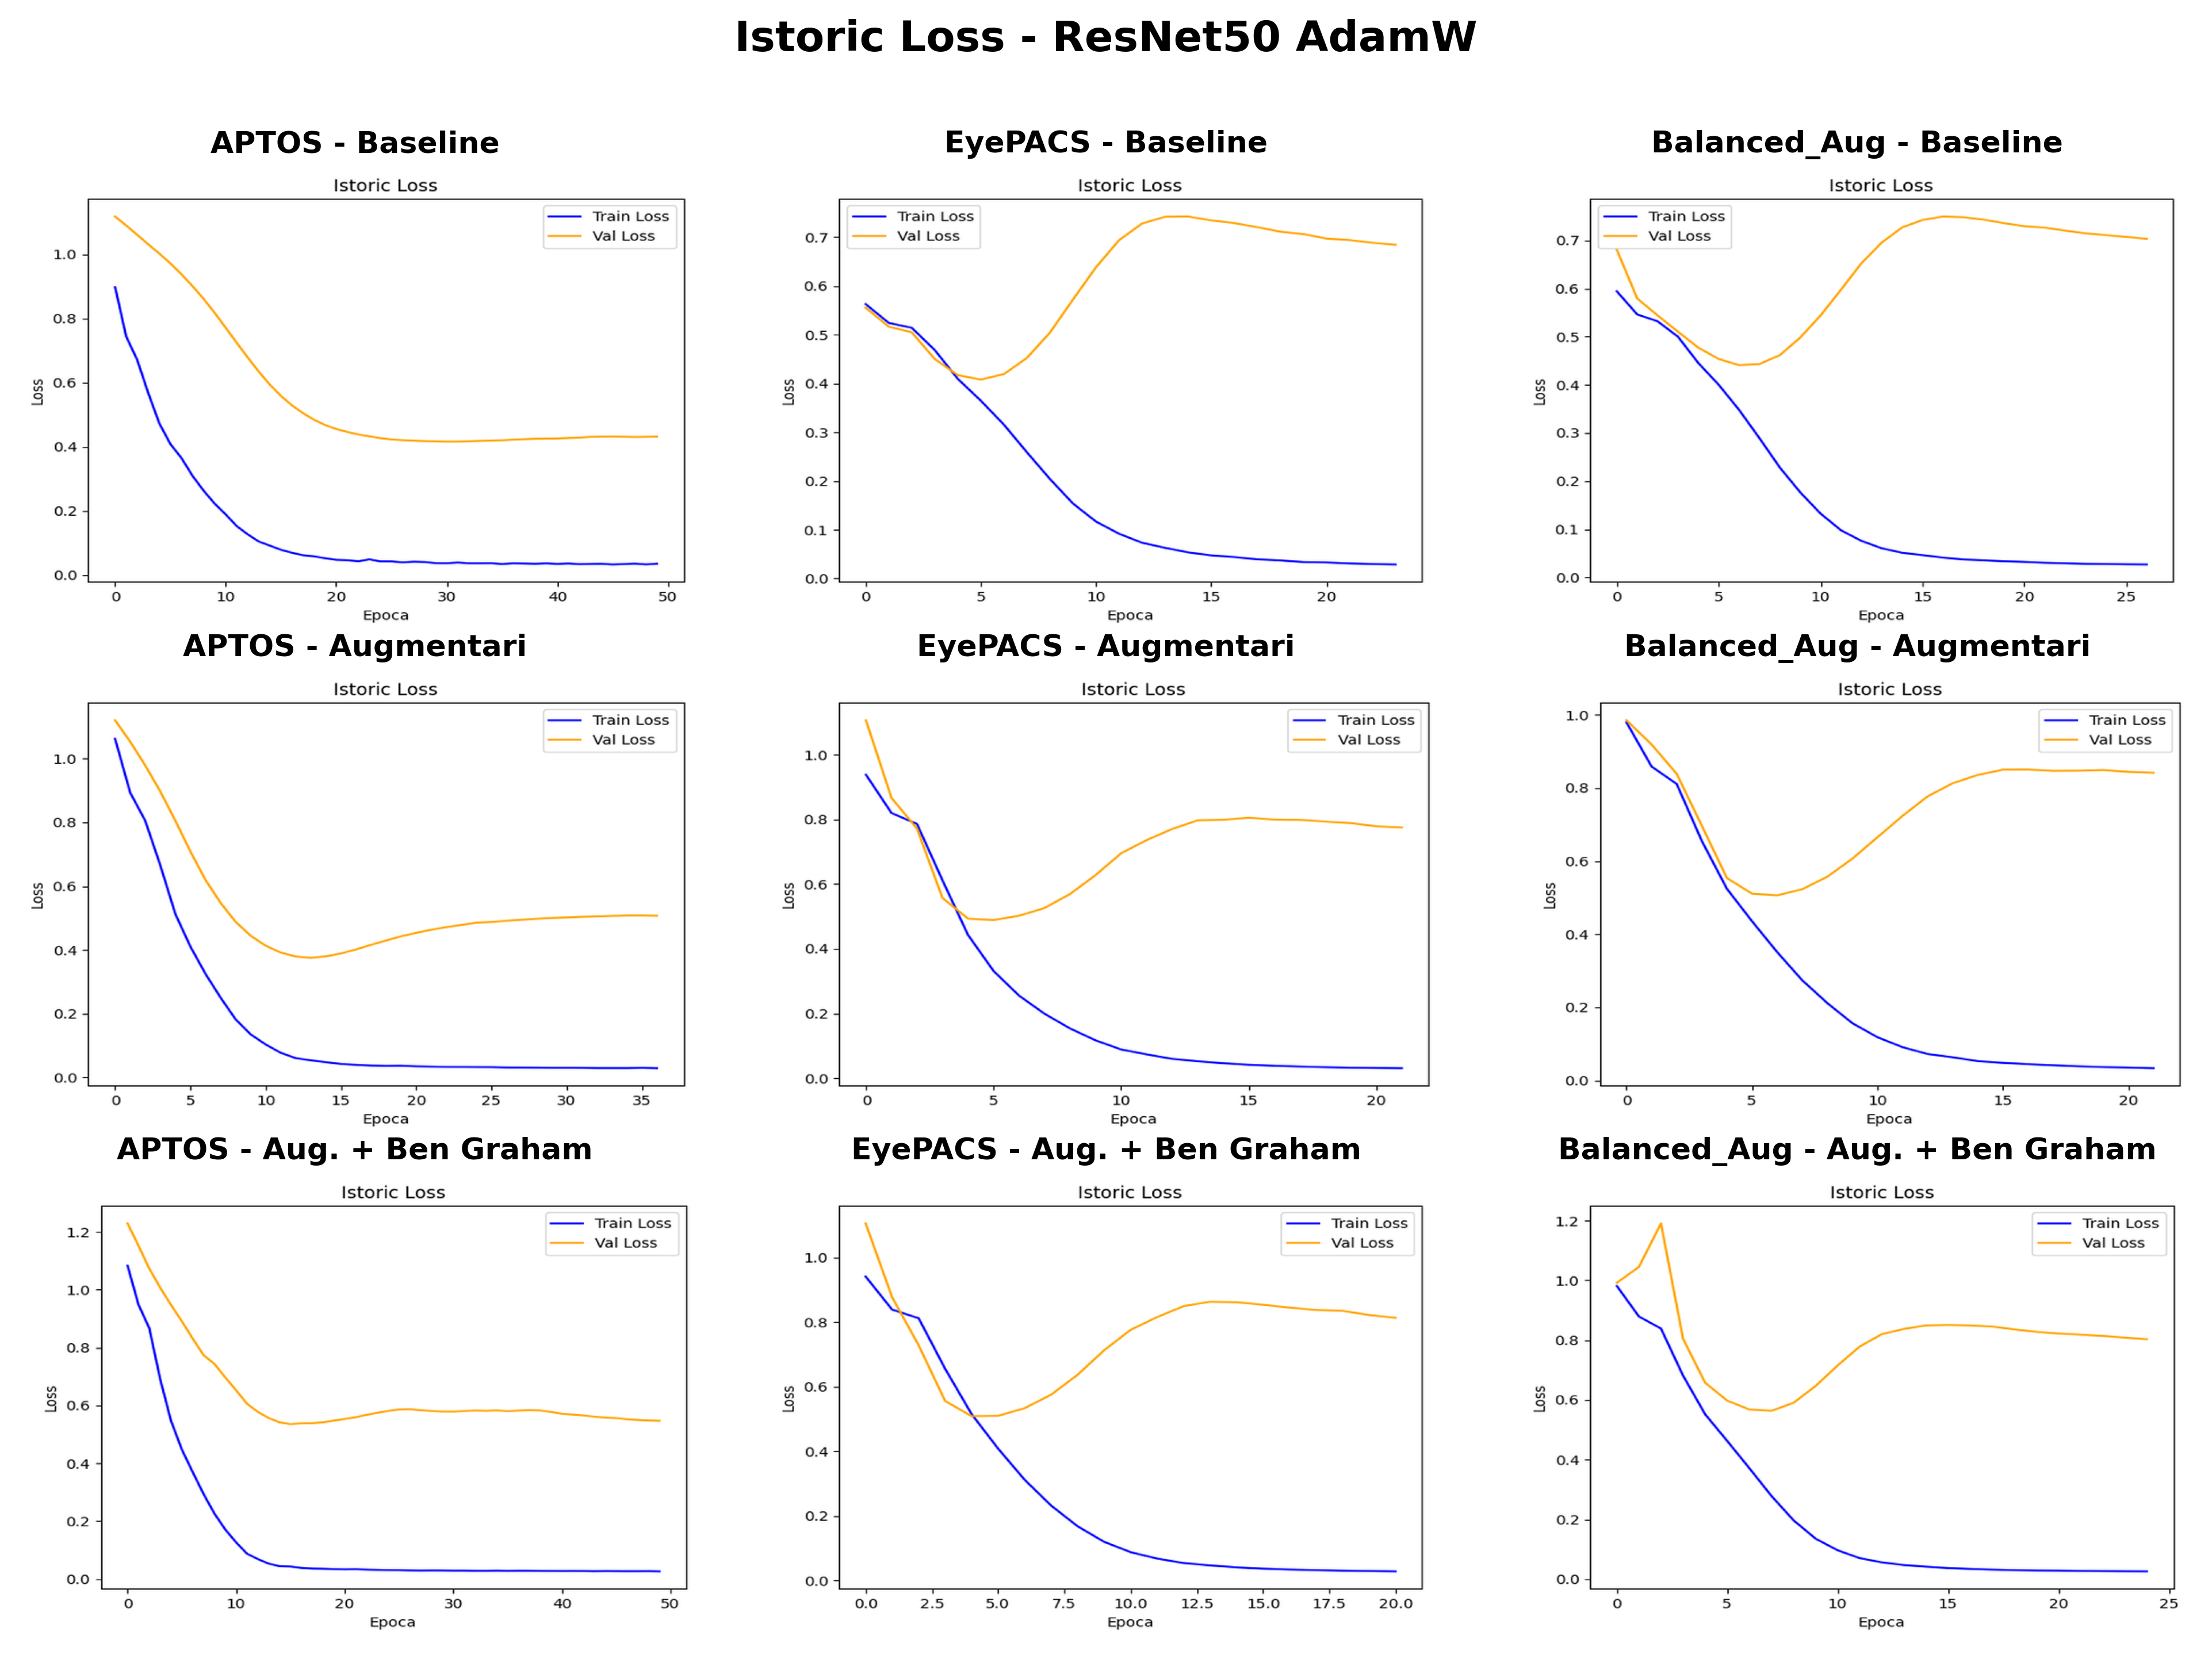
\includegraphics[width=0.9\textwidth]{Figuri/cap6_loss_resnet50_grid.png}
    \captionsetup{justification=centering}
    \caption{Istoricul loss-ului pentru ResNet50 cu AdamW pe APTOS, EyePACS și Balanced\_Aug.}
    \label{fig:cap6-loss-resnet50-grid}
\end{figure}

Pentru InceptionResNet-v2, istoricul loss-ului arată aceeași tensiune între învățarea pe train și
stabilitatea pe validare, dar rezultatele trebuie citite ca rezultate anterioare etapei finale de
fine-tuning. În această variantă, modelul nu beneficiază de aceleași ajustări aplicate ulterior
rulărilor ResNet50, iar arhitectura este mai complexă și mai sensibilă la alegerea ratei de învățare.
De aceea, în unele experimente pierderea pe validare crește în loc să scadă, chiar dacă la un moment dat
se stabilizează.
\bigskip

Creșterea \textit{val loss}-ului pentru InceptionResNet-v2 poate fi explicată prin mai mulți factori.
În primul rând, modelul are o capacitate mare și poate începe să se adapteze prea specific la imaginile
de antrenare, în timp ce validarea rămâne mai dificilă sau mai diferită vizual. În al doilea rând,
folosirea \textit{focal loss} face ca exemplele grele să aibă o contribuție mai mare la pierdere; dacă
setul de validare conține cazuri ambigue sau clase greu separabile, loss-ul poate crește chiar și atunci
când modelul începe să învețe anumite tipare utile. În al treilea rând, lipsa fine-tuning-ului în două
faze poate face actualizarea backbone-ului mai instabilă la început, deoarece capul de clasificare nu
este încă suficient de bine adaptat la problema curentă.
\bigskip

Faptul că loss-ul se stabilizează după o anumită perioadă arată că antrenarea nu este complet
divergentă, ci ajunge într-un regim relativ constant. Totuși, stabilizarea la o valoare mai ridicată
decât cea inițial dorită indică faptul că modelul nu reușește să transforme această stabilitate într-o
generalizare mai bună pe validare. Din acest motiv, InceptionResNet-v2 rămâne util ca experiment
comparativ, dar concluziile principale sunt formulate pe baza rulărilor ResNet50 actualizate, unde
fine-tuning-ul final oferă un protocol de antrenare mai controlat.
\bigskip

\begin{figure}[H] 
    \centering
    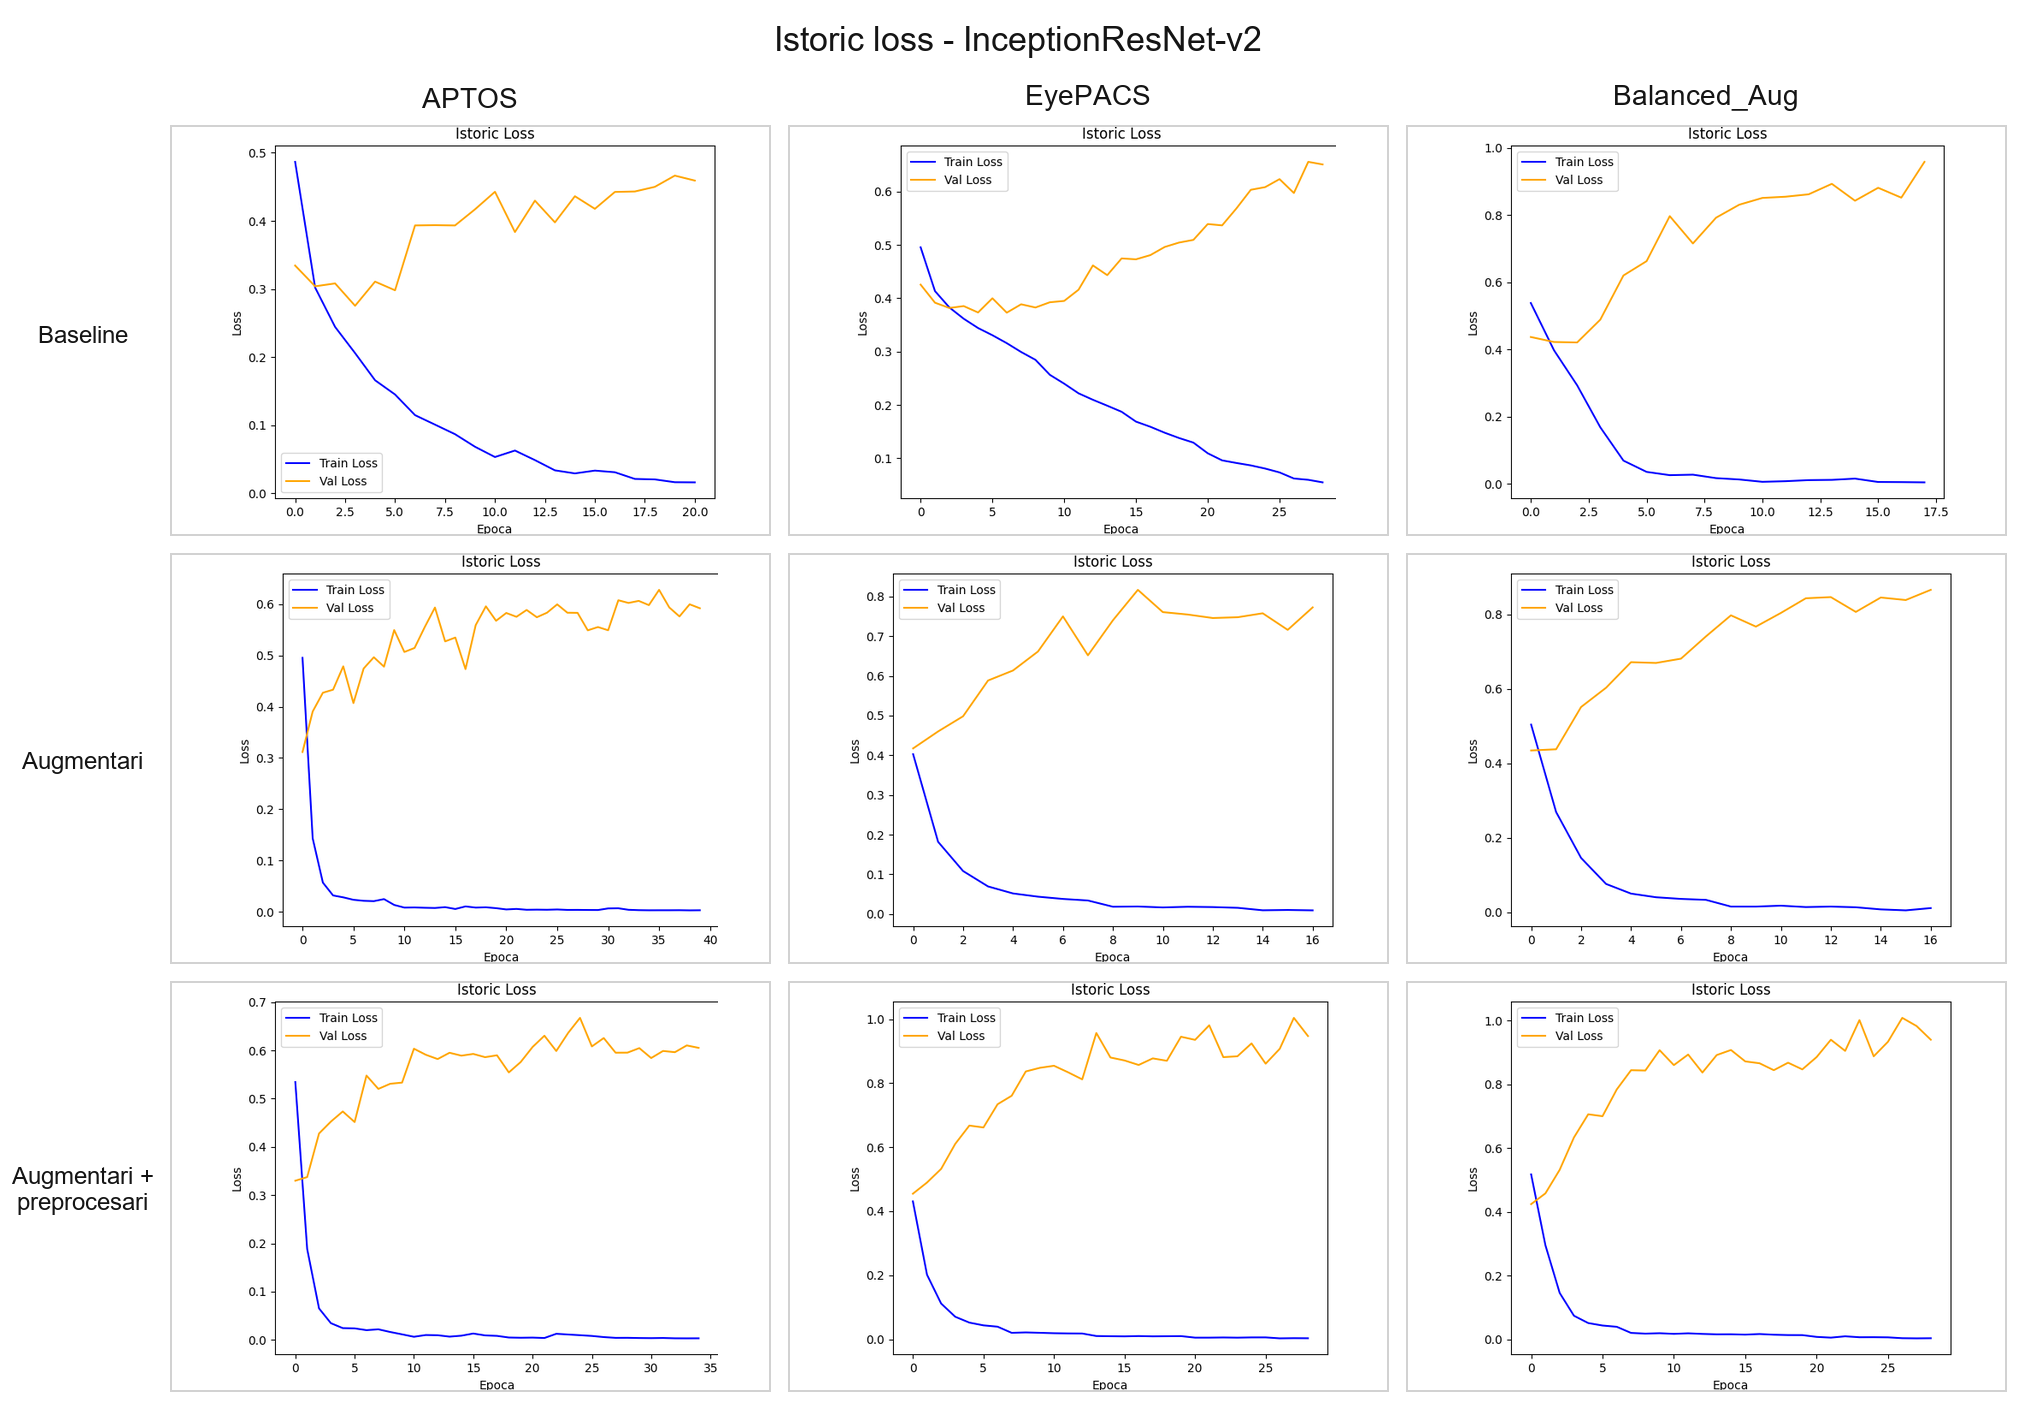
\includegraphics[width=0.9\textwidth]{Figuri/cap6_loss_incres_v2_grid.png}
    \captionsetup{justification=centering}
    \caption{Istoricul loss-ului pentru InceptionResNet-v2 pe APTOS, EyePACS și Balanced\_Aug.}
    \label{fig:cap6-loss-incres-grid}
\end{figure}

\section{Istoricul acurateții}

\ \ \ \ Figura \ref{fig:cap6-accuracy-resnet50-grid} prezintă evoluția acurateții pentru rulările
ResNet50 actualizate. În gradarea retinopatiei diabetice, acest scor global trebuie interpretat cu
prudență: modelul poate obține o acuratețe ridicată prin favorizarea claselor mai numeroase, fără să
recunoască suficient clasele intermediare sau cazurile severe. Acuratețea rămâne utilă ca indicator
rapid al progresului antrenării, însă concluziile sunt formulate în principal pe baza QWK, F1 pe clase
și matrici de confuzie.
\bigskip

În experimente, acuratețea de antrenare crește rapid în majoritatea cazurilor, ceea ce arată că
modelul reușește să învețe exemplele disponibile. Diferența față de acuratețea de validare este însă
esențială pentru interpretare: un scor ridicat pe antrenare nu este suficient dacă validarea rămâne
instabilă sau plafonată.
\bigskip

Rezultatele finale confirmă această limitare: pe APTOS se obțin acurateți de \(0.82\), \(0.79\) și
\(0.81\) pentru baseline, augmentări și augmentări cu Ben Graham, în timp ce pe EyePACS valorile sunt
\(0.77\), \(0.74\) și \(0.73\). Pentru Balanced\_Aug, acuratețea scade de la \(0.75\) la \(0.72\) și
\(0.69\), deși macro-F1 crește de la \(0.42\) la \(0.49\), respectiv \(0.51\). Prin urmare,
augmentările și preprocesarea nu trebuie evaluate doar prin acuratețe, ci prin distribuția erorilor pe
clase și prin stabilitatea metricilor ordinale.

\begin{figure}[H]
    \centering
    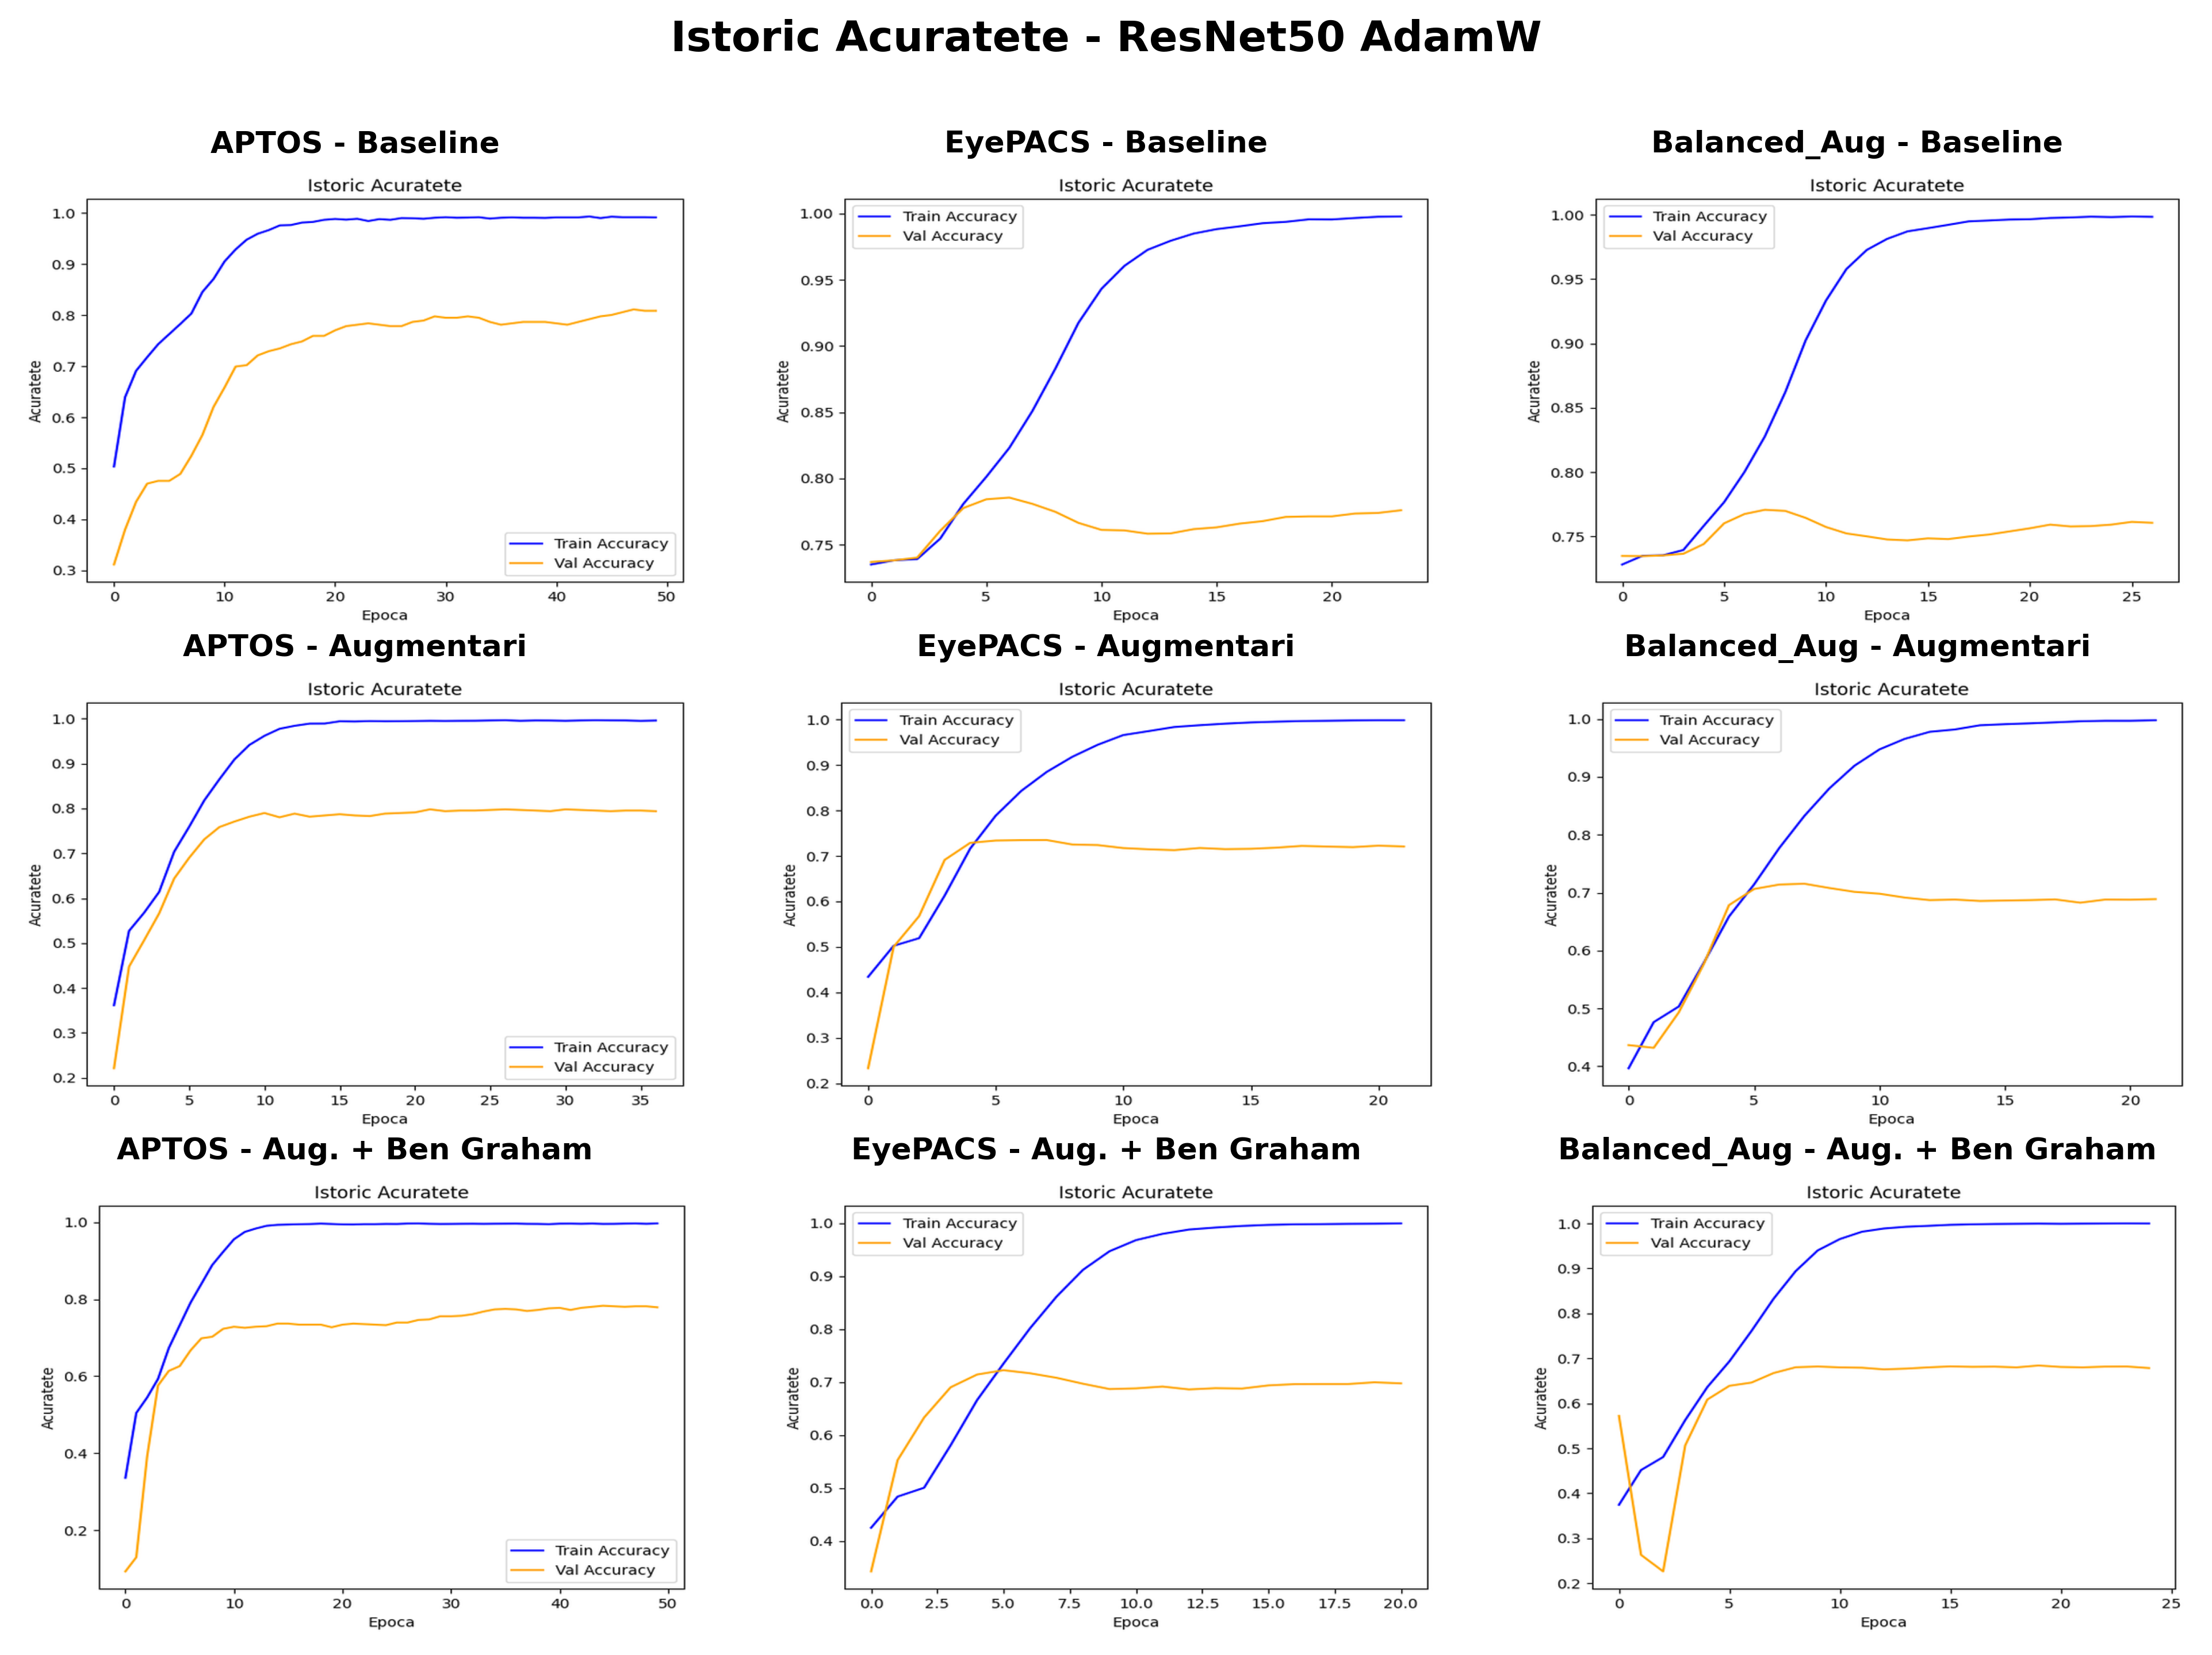
\includegraphics[width=0.95\textwidth]{Figuri/cap6_accuracy_resnet50_grid.png}
    \captionsetup{justification=centering}
    \caption{Istoricul acurateții pentru ResNet50 cu AdamW pe cele nouă variante de experimente.}
    \label{fig:cap6-accuracy-resnet50-grid}
\end{figure}

\section{Istoricul scorului QWK}

\ \ \ \ Pentru gradarea retinopatiei diabetice, acuratețea nu surprinde complet severitatea erorilor.
De aceea, figura \ref{fig:cap6-qwk-resnet50-grid} urmărește scorul QWK, o metrică mai potrivită
pentru clase ordinale. O confuzie între clase vecine, de exemplu
1 și 2, este mai puțin severă decât o confuzie între clasa 0 și clasa 4, iar QWK reflectă această
diferență.
\bigskip

Istoricul QWK arată cât de stabil devine modelul în raport cu ordinea clinică a claselor. În
experimentele în care QWK crește odată cu antrenarea, modelul nu doar clasifică mai multe imagini
corect, ci învață o structură mai apropiată de severitatea bolii. Această metrică este relevantă
pentru lucrare deoarece sistemul final nu urmărește doar o etichetă numerică, ci o estimare a
stadiului retinopatiei diabetice.
\bigskip

QWK este urmărit deoarece clasele au ordine clinică. Pentru ResNet50, acest grafic arată dacă modelul
învață nu doar etichete corecte, ci și o separare coerentă între gradele de severitate.
\bigskip

\begin{figure}[H]
    \centering
    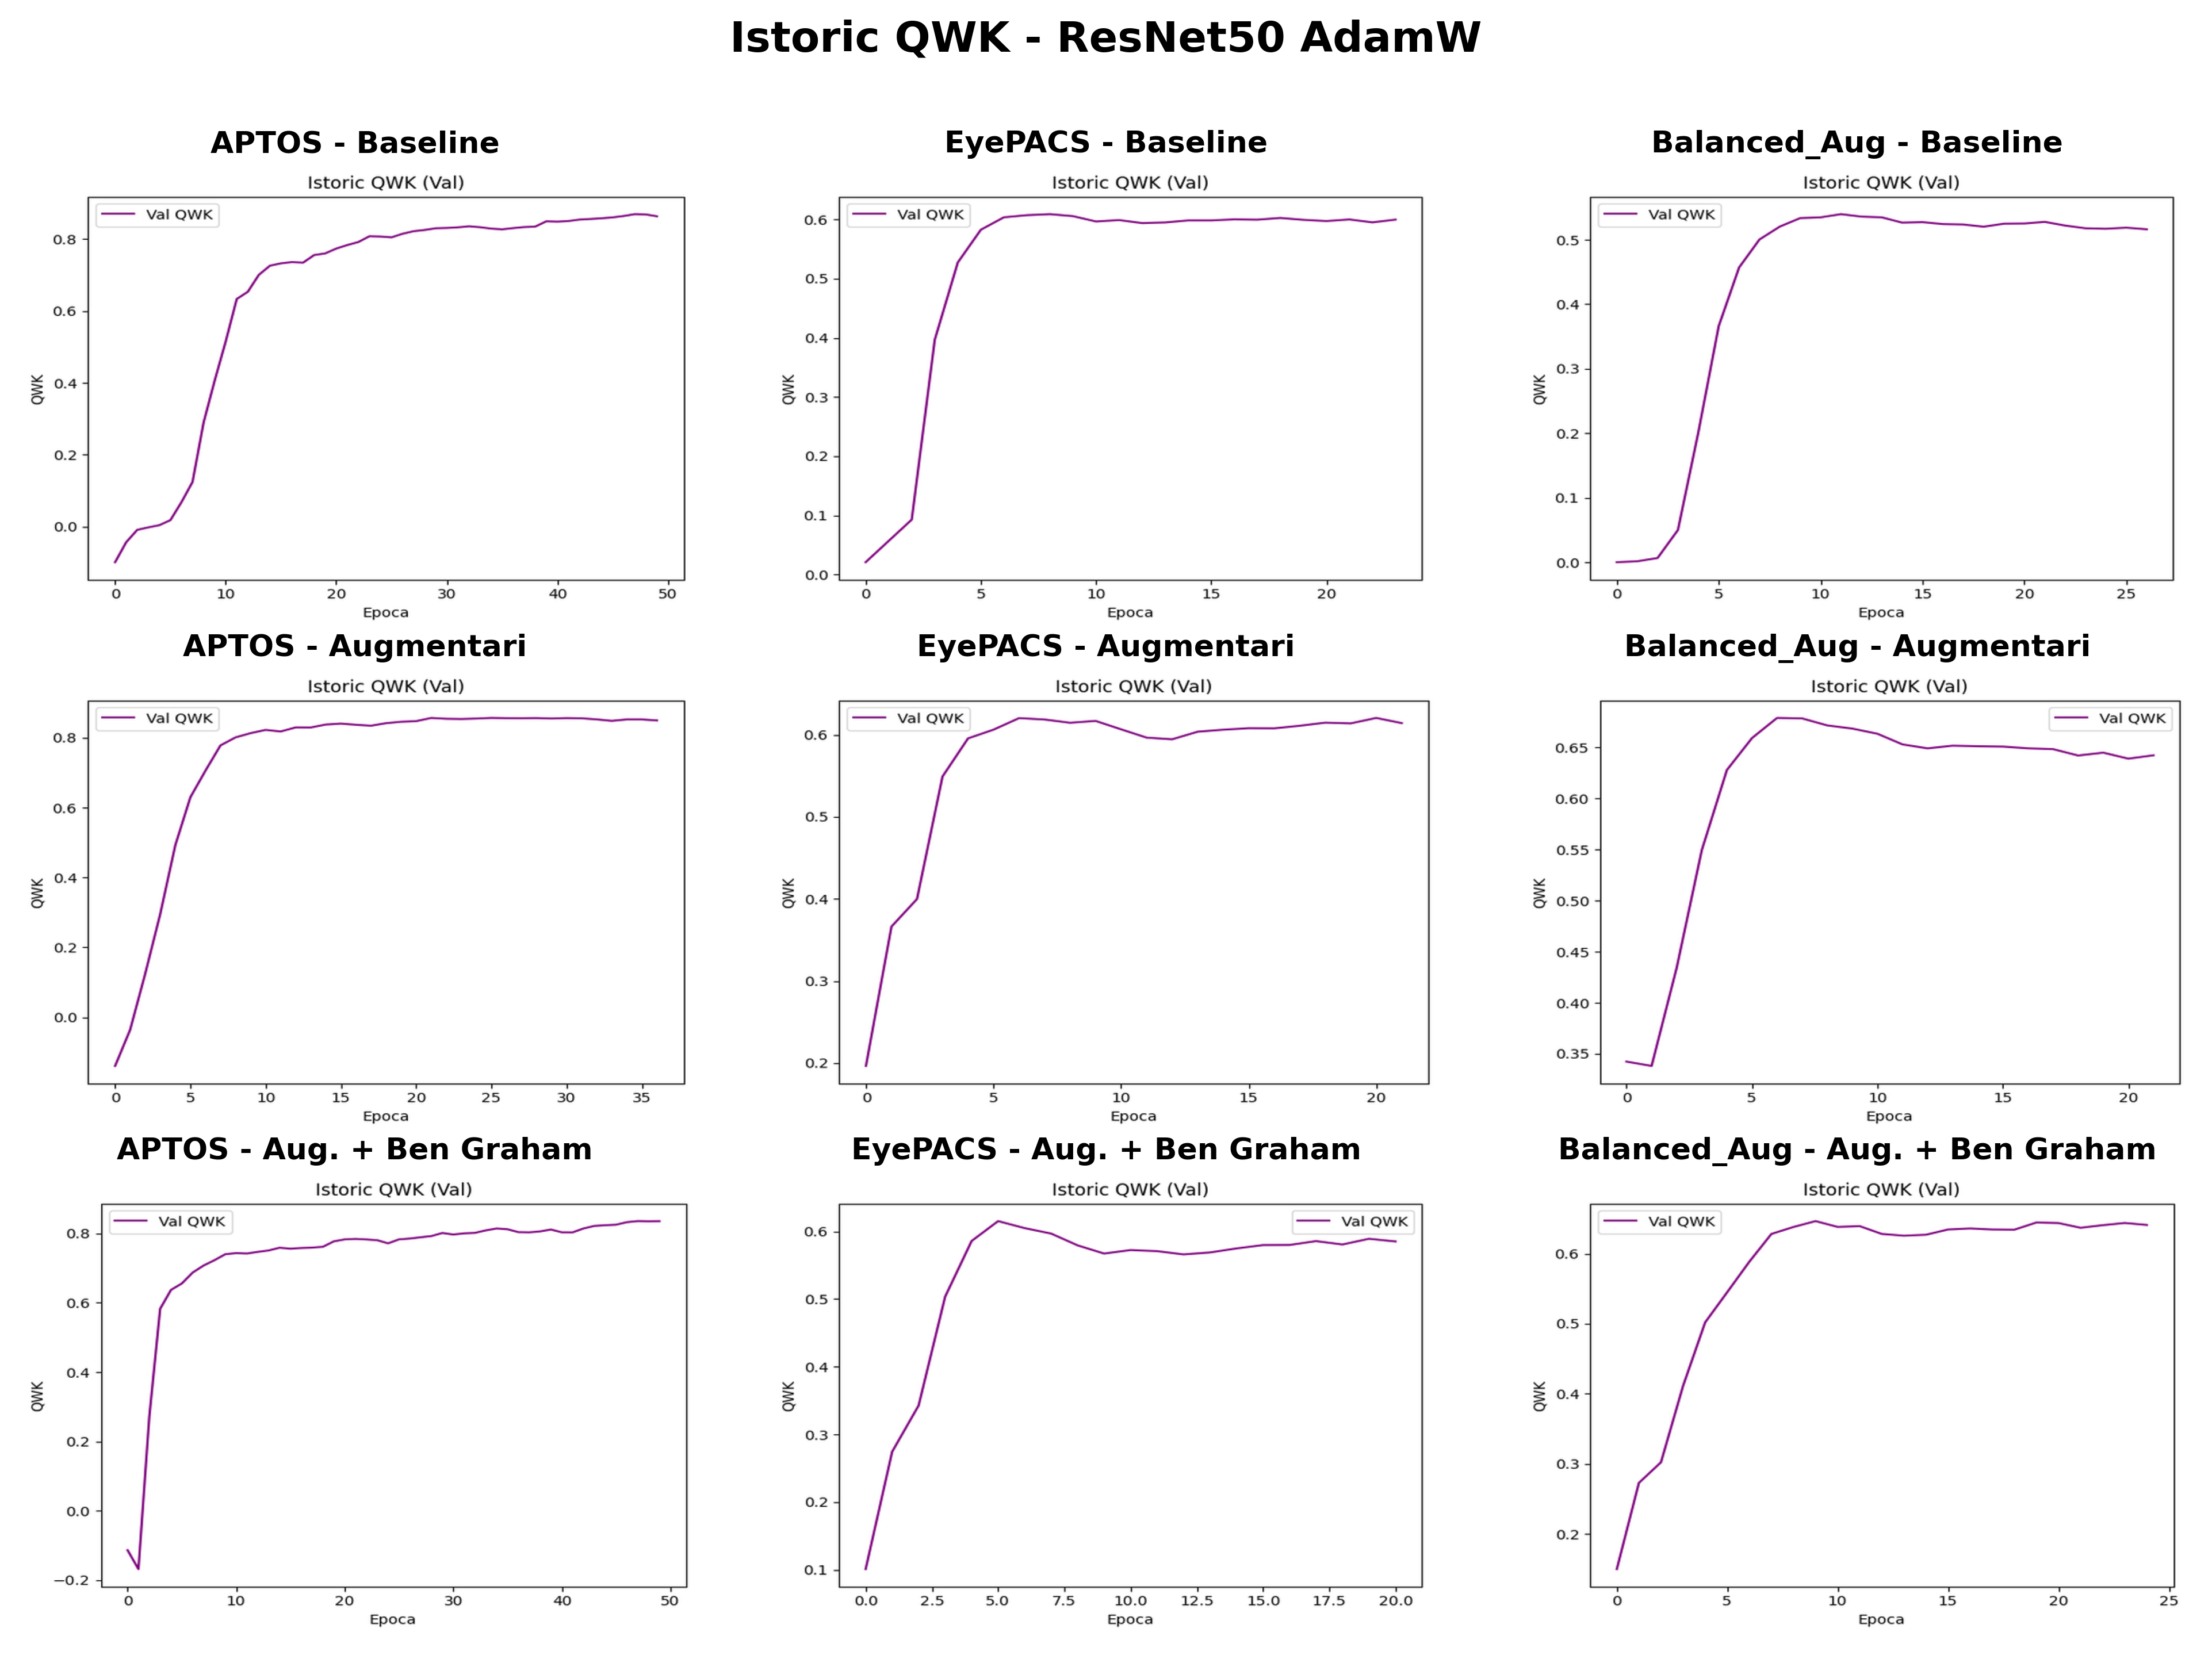
\includegraphics[width=0.95\textwidth]{Figuri/cap6_qwk_resnet50_grid.png}
    \captionsetup{justification=centering}
    \caption{Istoricul scorului QWK pentru ResNet50 cu AdamW pe cele nouă variante de experimente.}
    \label{fig:cap6-qwk-resnet50-grid}
\end{figure}

\ \ \ \ Din figura \ref{fig:cap6-qwk-resnet50-grid} se observă că evoluția QWK nu este identică pentru
toate combinațiile de set de date și strategie de antrenare. Pe APTOS, curbele ajung în zona
\(0.83\)--\(0.87\), semn că modelul păstrează mai bine ordinea severității. Pe EyePACS, QWK se
stabilizează în jurul intervalului \(0.59\)--\(0.62\), iar pe Balanced\_Aug valorile sunt mai sensibile
la etapa de pregătire a datelor, cu un comportament mai bun pentru variantele augmentate decât pentru
baseline. Diferența față de acuratețe arată că o scădere a scorului global nu înseamnă neapărat o
degradare ordinală uniformă.
\bigskip

\ \ \ \ Un aspect important este că QWK penalizează mai puternic confuziile între clase îndepărtate.
De aceea, chiar dacă acuratețea poate părea apropiată între două experimente, o curbă QWK mai bună
indică faptul că modelul greșește mai rar severitatea într-un mod clinic grav. Pentru această lucrare,
graficul este util deoarece arată nu doar dacă ResNet50 ajunge la performanțe bune, ci și dacă
învățarea este stabilă în raport cu ordinea naturală a claselor de retinopatie diabetică.
\bigskip

\section{Precision, recall și F1 pe clase}

\ \ \ \ Figura \ref{fig:cap6-prf1-grid} prezintă valorile precision, recall și F1 pentru fiecare
clasă. Această analiză este mai informativă decât acuratețea globală deoarece arată unde modelul
recunoaște bine imaginile și unde apar dificultăți. În noile rulări, APTOS are cele mai bune scoruri
pe clasele intermediare: F1 pentru clasa 1 este \(0.56\), \(0.51\) și \(0.62\), iar pentru clasa 2 este
\(0.73\), \(0.73\) și \(0.76\), în ordinea baseline, augmentări și augmentări cu Ben Graham. Pentru
EyePACS și Balanced\_Aug, clasa 1 rămâne cea mai dificilă, dar varianta Balanced\_Aug cu Ben Graham
ridică F1-ul clasei 1 la \(0.25\), față de \(0.07\) în baseline.
\bigskip

Prin raportarea pe clase se observă mai clar efectul augmentărilor. Dacă augmentările îmbunătățesc
recall-ul pentru clasele rare, modelul devine mai util în scenarii în care ratarea cazurilor
patologice este costisitoare. Dacă precision-ul scade, apare riscul de alarme false. Din acest motiv,
scorurile pe clase trebuie analizate împreună cu matricele de confuzie, nu izolat. În ansamblu,
graficele F1 arată că principala dificultate nu este separarea extremelor, ci delimitarea fină a
stadiilor apropiate. Clasele 1 și 2 sunt cele mai importante de urmărit, deoarece diferențele vizuale
dintre absența bolii, formele ușoare și formele moderate pot fi subtile.
\bigskip

\begin{figure}[H]
    \centering
    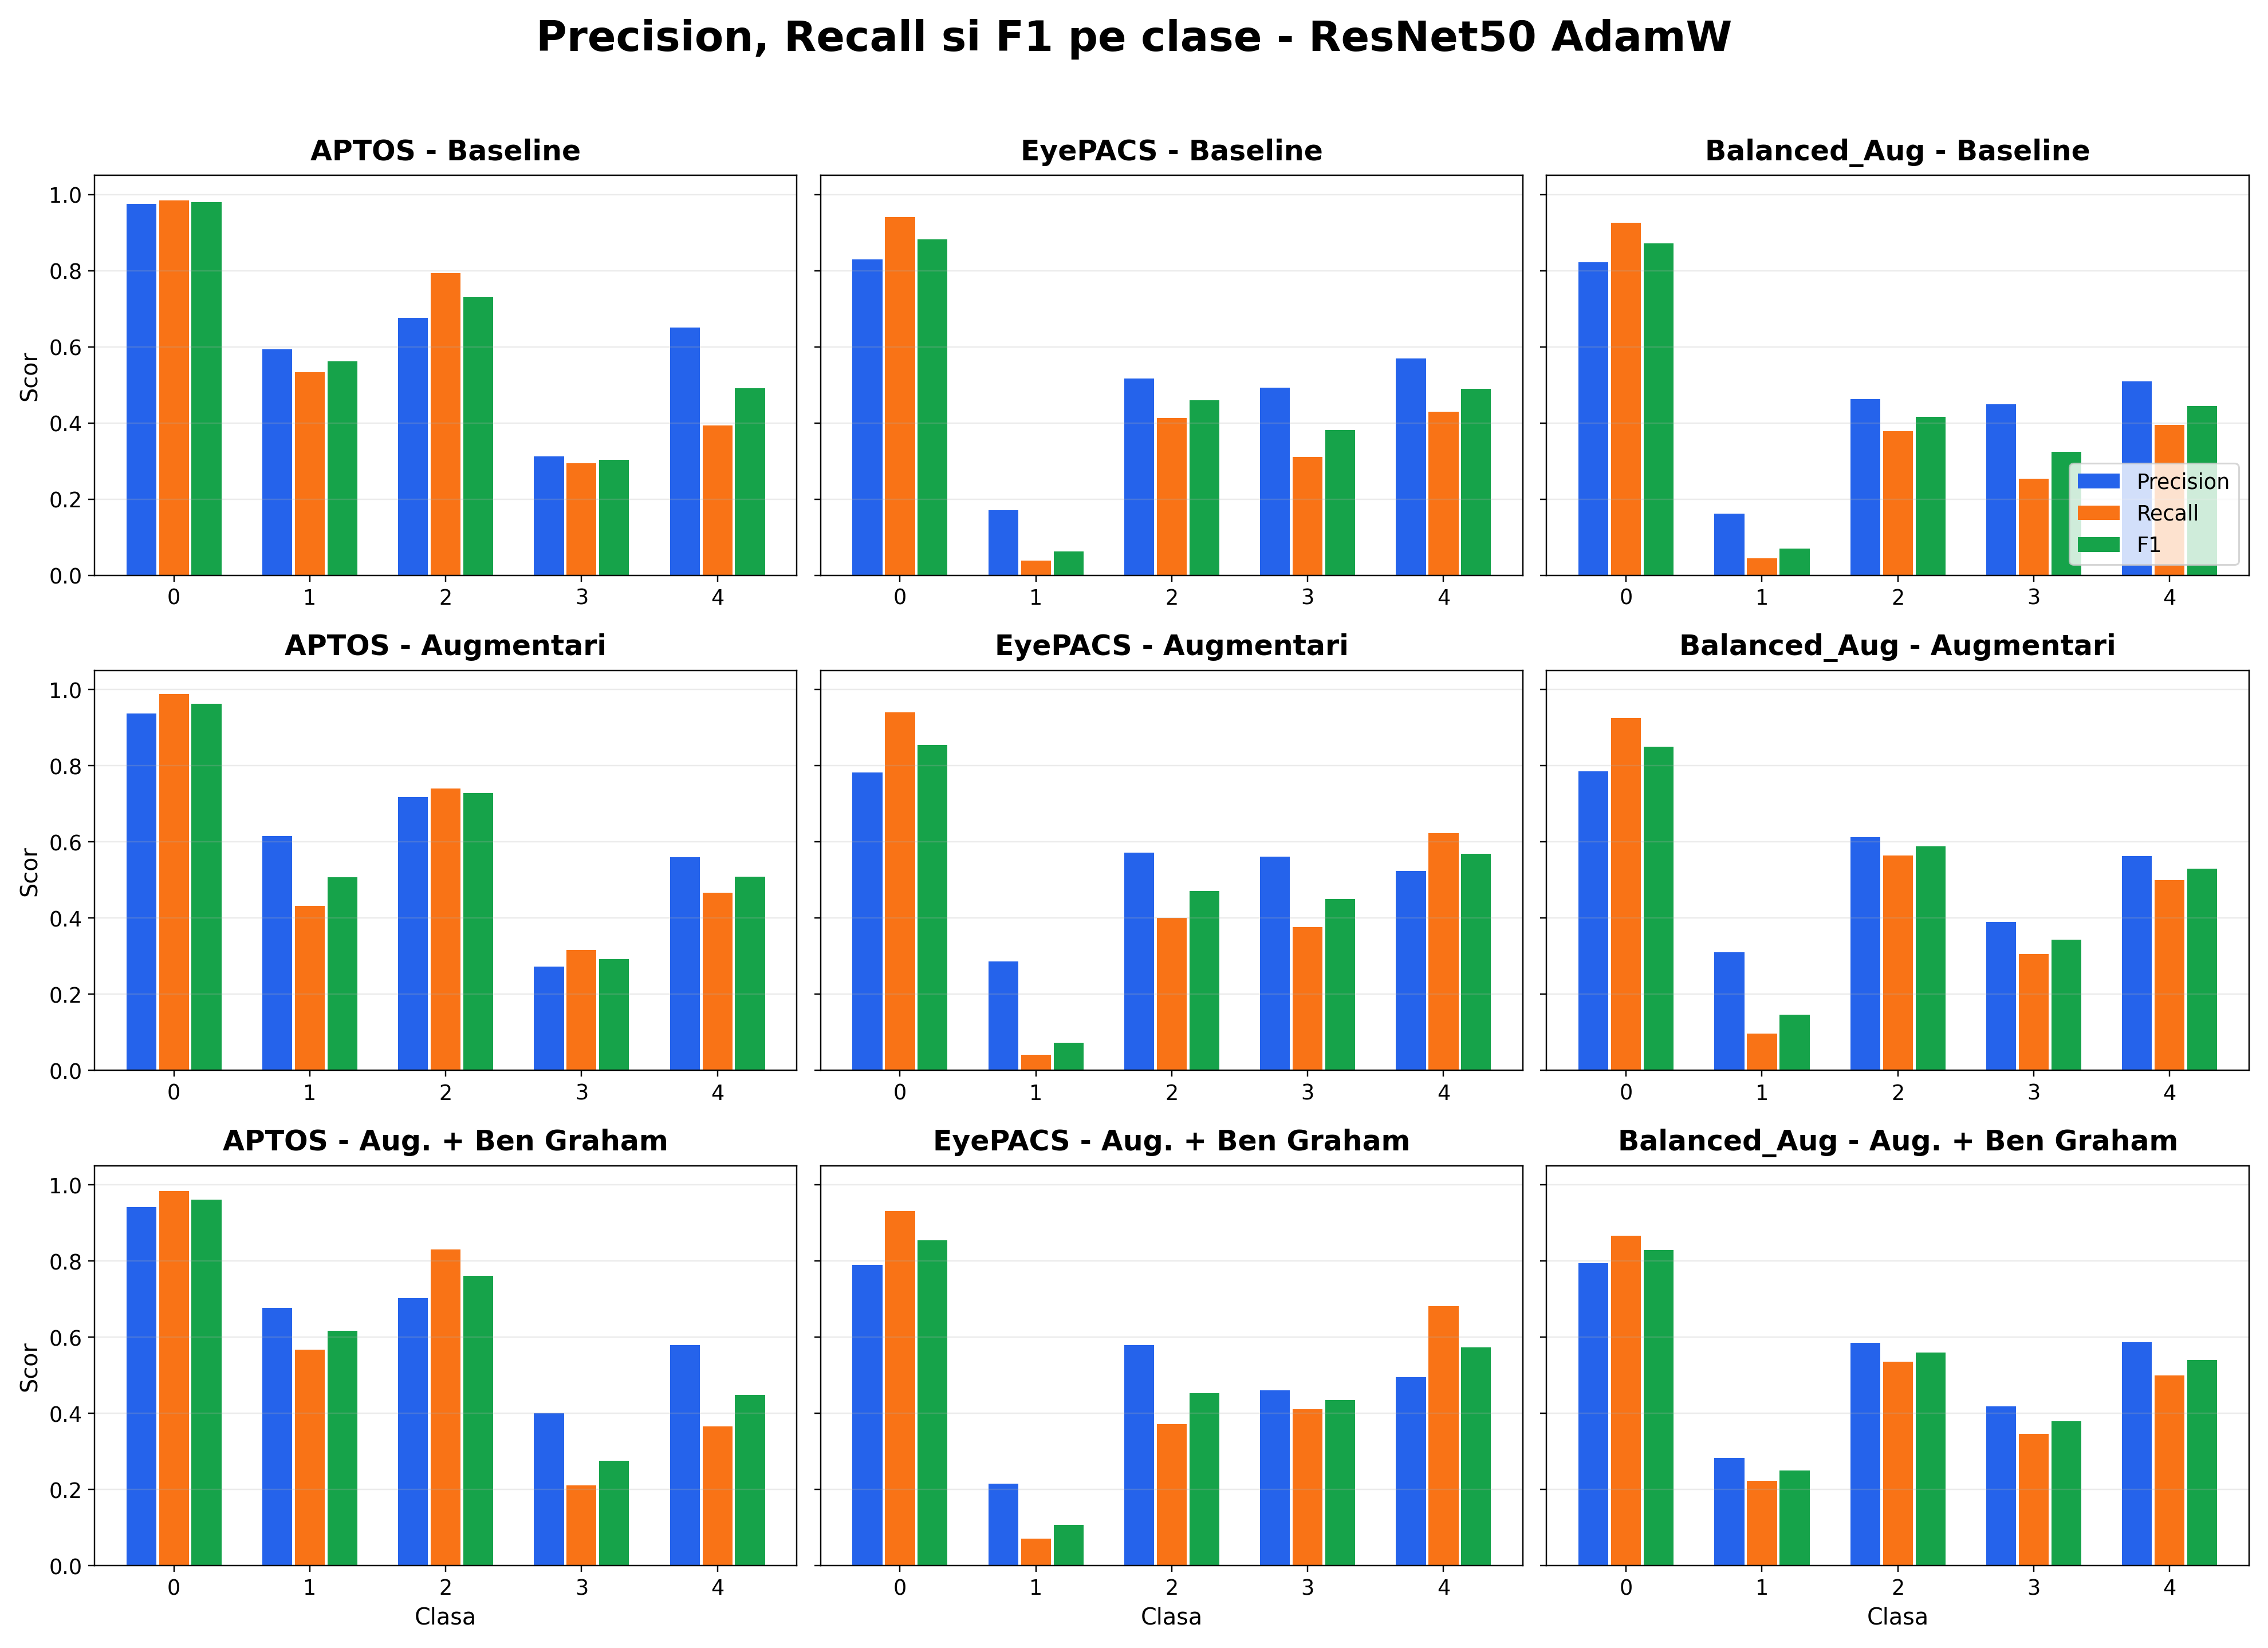
\includegraphics[width=0.98\textwidth]{Figuri/cap6_prf1_grid.png}
    \captionsetup{justification=centering}
    \caption{Precision, recall și F1 pe clase pentru cele nouă experimente ResNet50 cu AdamW.}
    \label{fig:cap6-prf1-grid}
\end{figure}

\section{Matricele de confuzie}

\ \ \ \ Matricele de confuzie din figura \ref{fig:cap6-confusion-grid} arată explicit tipurile de
erori produse de model. Pentru retinopatia diabetică, nu toate erorile au aceeași semnificație:
confuziile între clase apropiate pot reflecta ambiguitatea naturală a imaginilor, în timp ce
confuziile între clasa 0 și clasele avansate indică o problemă mai gravă de detecție.
\bigskip

Aceste rezultate confirmă importanța curățării seturilor de date și a controlului asupra
augmentărilor. Atunci când imaginile augmentate sunt distribuite incorect între partiții sau când
preprocesările nu sunt aplicate consecvent, matricea de confuzie poate sugera performanțe artificiale
sau erori greu de interpretat. De aceea, în această lucrare, pregătirea dataseturilor a fost tratată
ca o etapă experimentală centrală, nu doar ca un pas auxiliar înainte de antrenare.
\newline 

\ \ \ \ Pentru claritate, figura păstrează doar matricile absolute, nu și variantele normalizate. Valorile
absolute fac mai ușor de observat unde se concentrează efectiv erorile. Se remarcă un tipar comun:
o parte din imaginile din clasele 1 și 2 sunt prezise ca 0, ceea ce arată că modelul are dificultăți
în delimitarea cazurilor incipiente față de absența bolii. Totuși, clasele marginale nu sunt amestecate
puternic între ele: imaginile sănătoase nu sunt confundate masiv cu stadiile severe, iar clasa 4 nu
este trimisă frecvent direct către clasa 0. Această observație este importantă deoarece susține
trecerea la un sistem în două faze: mai întâi o decizie binară sănătos/patologic, apoi o clasificare
mai fină doar pentru imaginile patologice.
Matricele de confuzie indică tipul erorilor, nu doar numărul lor. În această figură sunt păstrate
doar valorile absolute, pentru a evidenția direct confuziile dintre clasele reale și cele prezise.
În rulările actualizate, APTOS rămâne cel mai echilibrat: în varianta cu Ben Graham, clasa 2 are
\(83\) predicții corecte din \(100\), iar clasa 1 ajunge la \(21\) din \(37\). Pe EyePACS și
Balanced\_Aug se observă în continuare absorbția claselor 1 și 2 în clasa 0, ceea ce explică diferența
dintre acuratețea globală și scorul F1.

\begin{figure}[H]
    \centering
    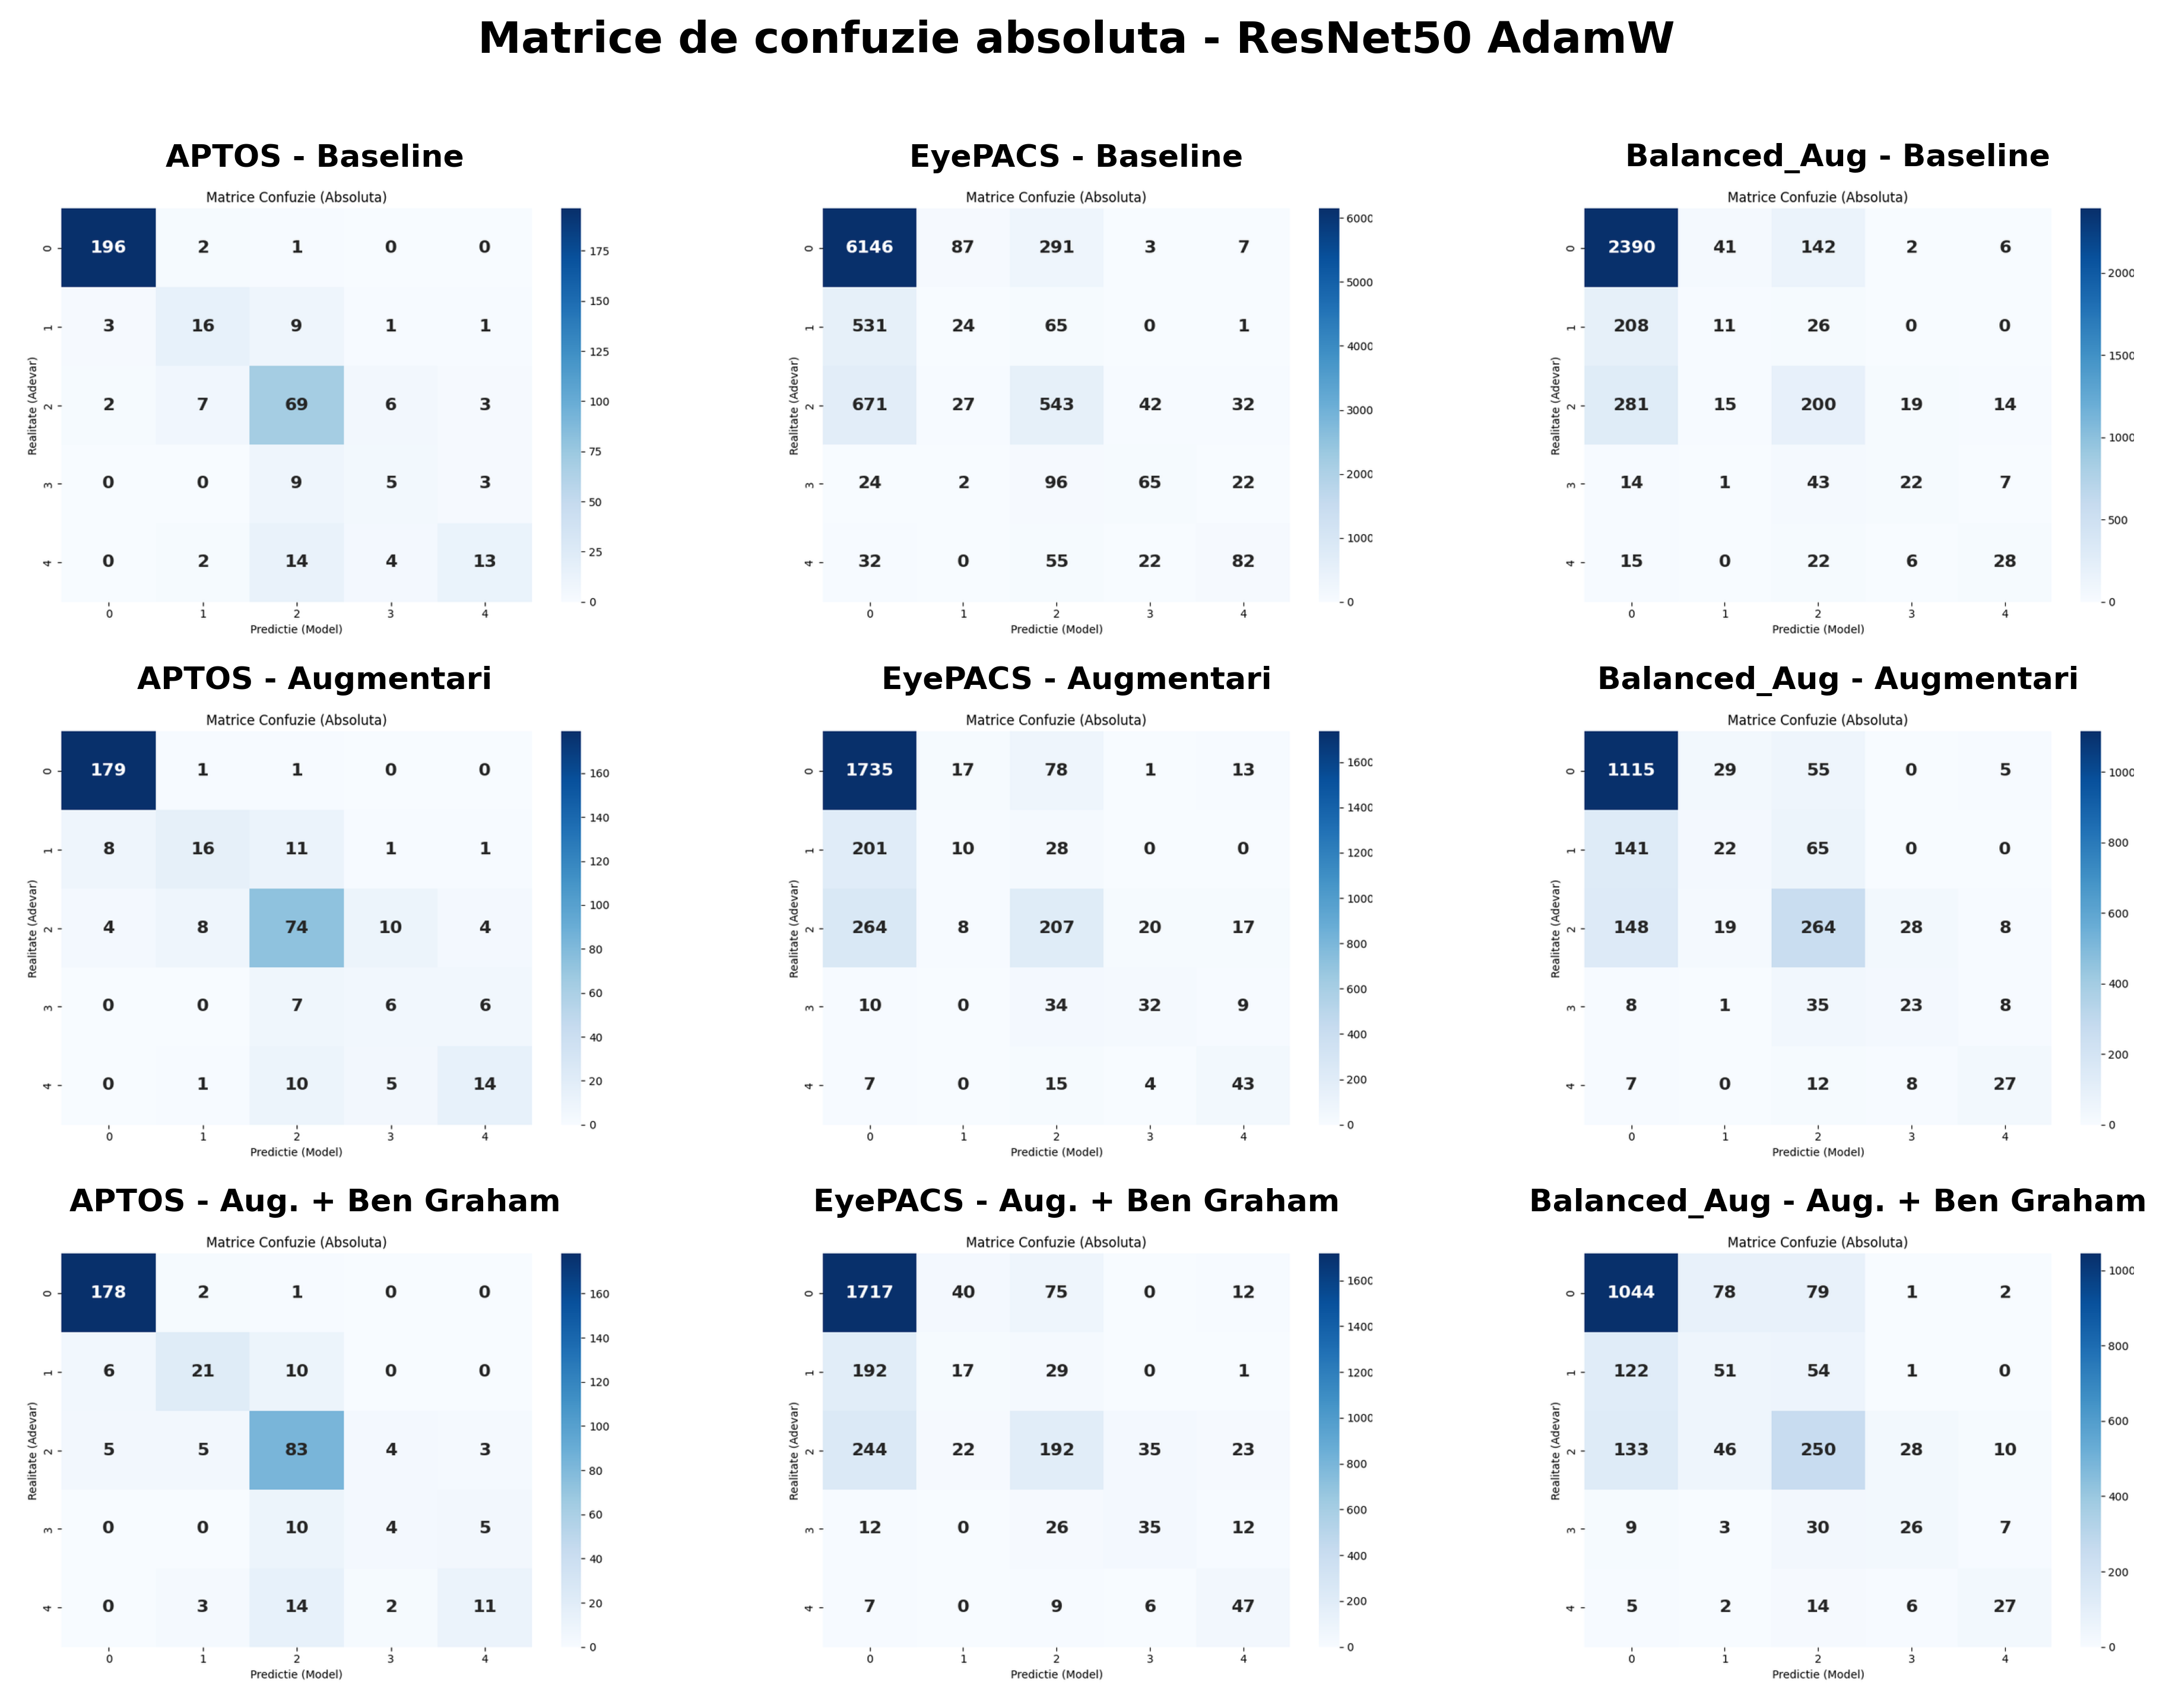
\includegraphics[width=0.92\textwidth]{Figuri/cap6_confusion_grid_abs.png}
    \captionsetup{justification=centering}
    \caption{Matricele de confuzie absolute pentru ResNet50 cu AdamW pe cele trei dataseturi și cele trei configurații.}
    \label{fig:cap6-confusion-grid}
\end{figure}

\section{Curbele ROC multiclasă}

\ \ \ \ Figura \ref{fig:cap6-roc-grid} prezintă curbele ROC multiclasă. Acestea sunt utile pentru a
observa capacitatea modelului de a separa fiecare clasă în raport cu celelalte, independent de un
prag fix de decizie. În context multiclasă, curbele ROC completează analiza pe clase și arată dacă
modelul produce scoruri probabilistice coerente, chiar și atunci când predicția finală este greșită.
\bigskip

Compararea pe coloane indică diferențe între domeniile vizuale ale seturilor de date. APTOS,
EyePACS și Balanced\_Aug nu au aceeași distribuție a imaginilor, iar curbele ROC reflectă această
variație. Compararea pe rânduri arată efectul etapelor de lucru asupra datelor: augmentările și
preprocesările pot schimba separabilitatea claselor, dar aceste lucruri trebuie verificate pentru
fiecare dataset.
\bigskip

Curbele ROC multiclasă arată capacitatea modelului de a separa fiecare clasă față de celelalte. 
Ele completează matricele de confuzie deoarece analizează scorurile probabilistice, nu doar predicția finală.
\bigskip

\begin{figure}[H]
    \centering
    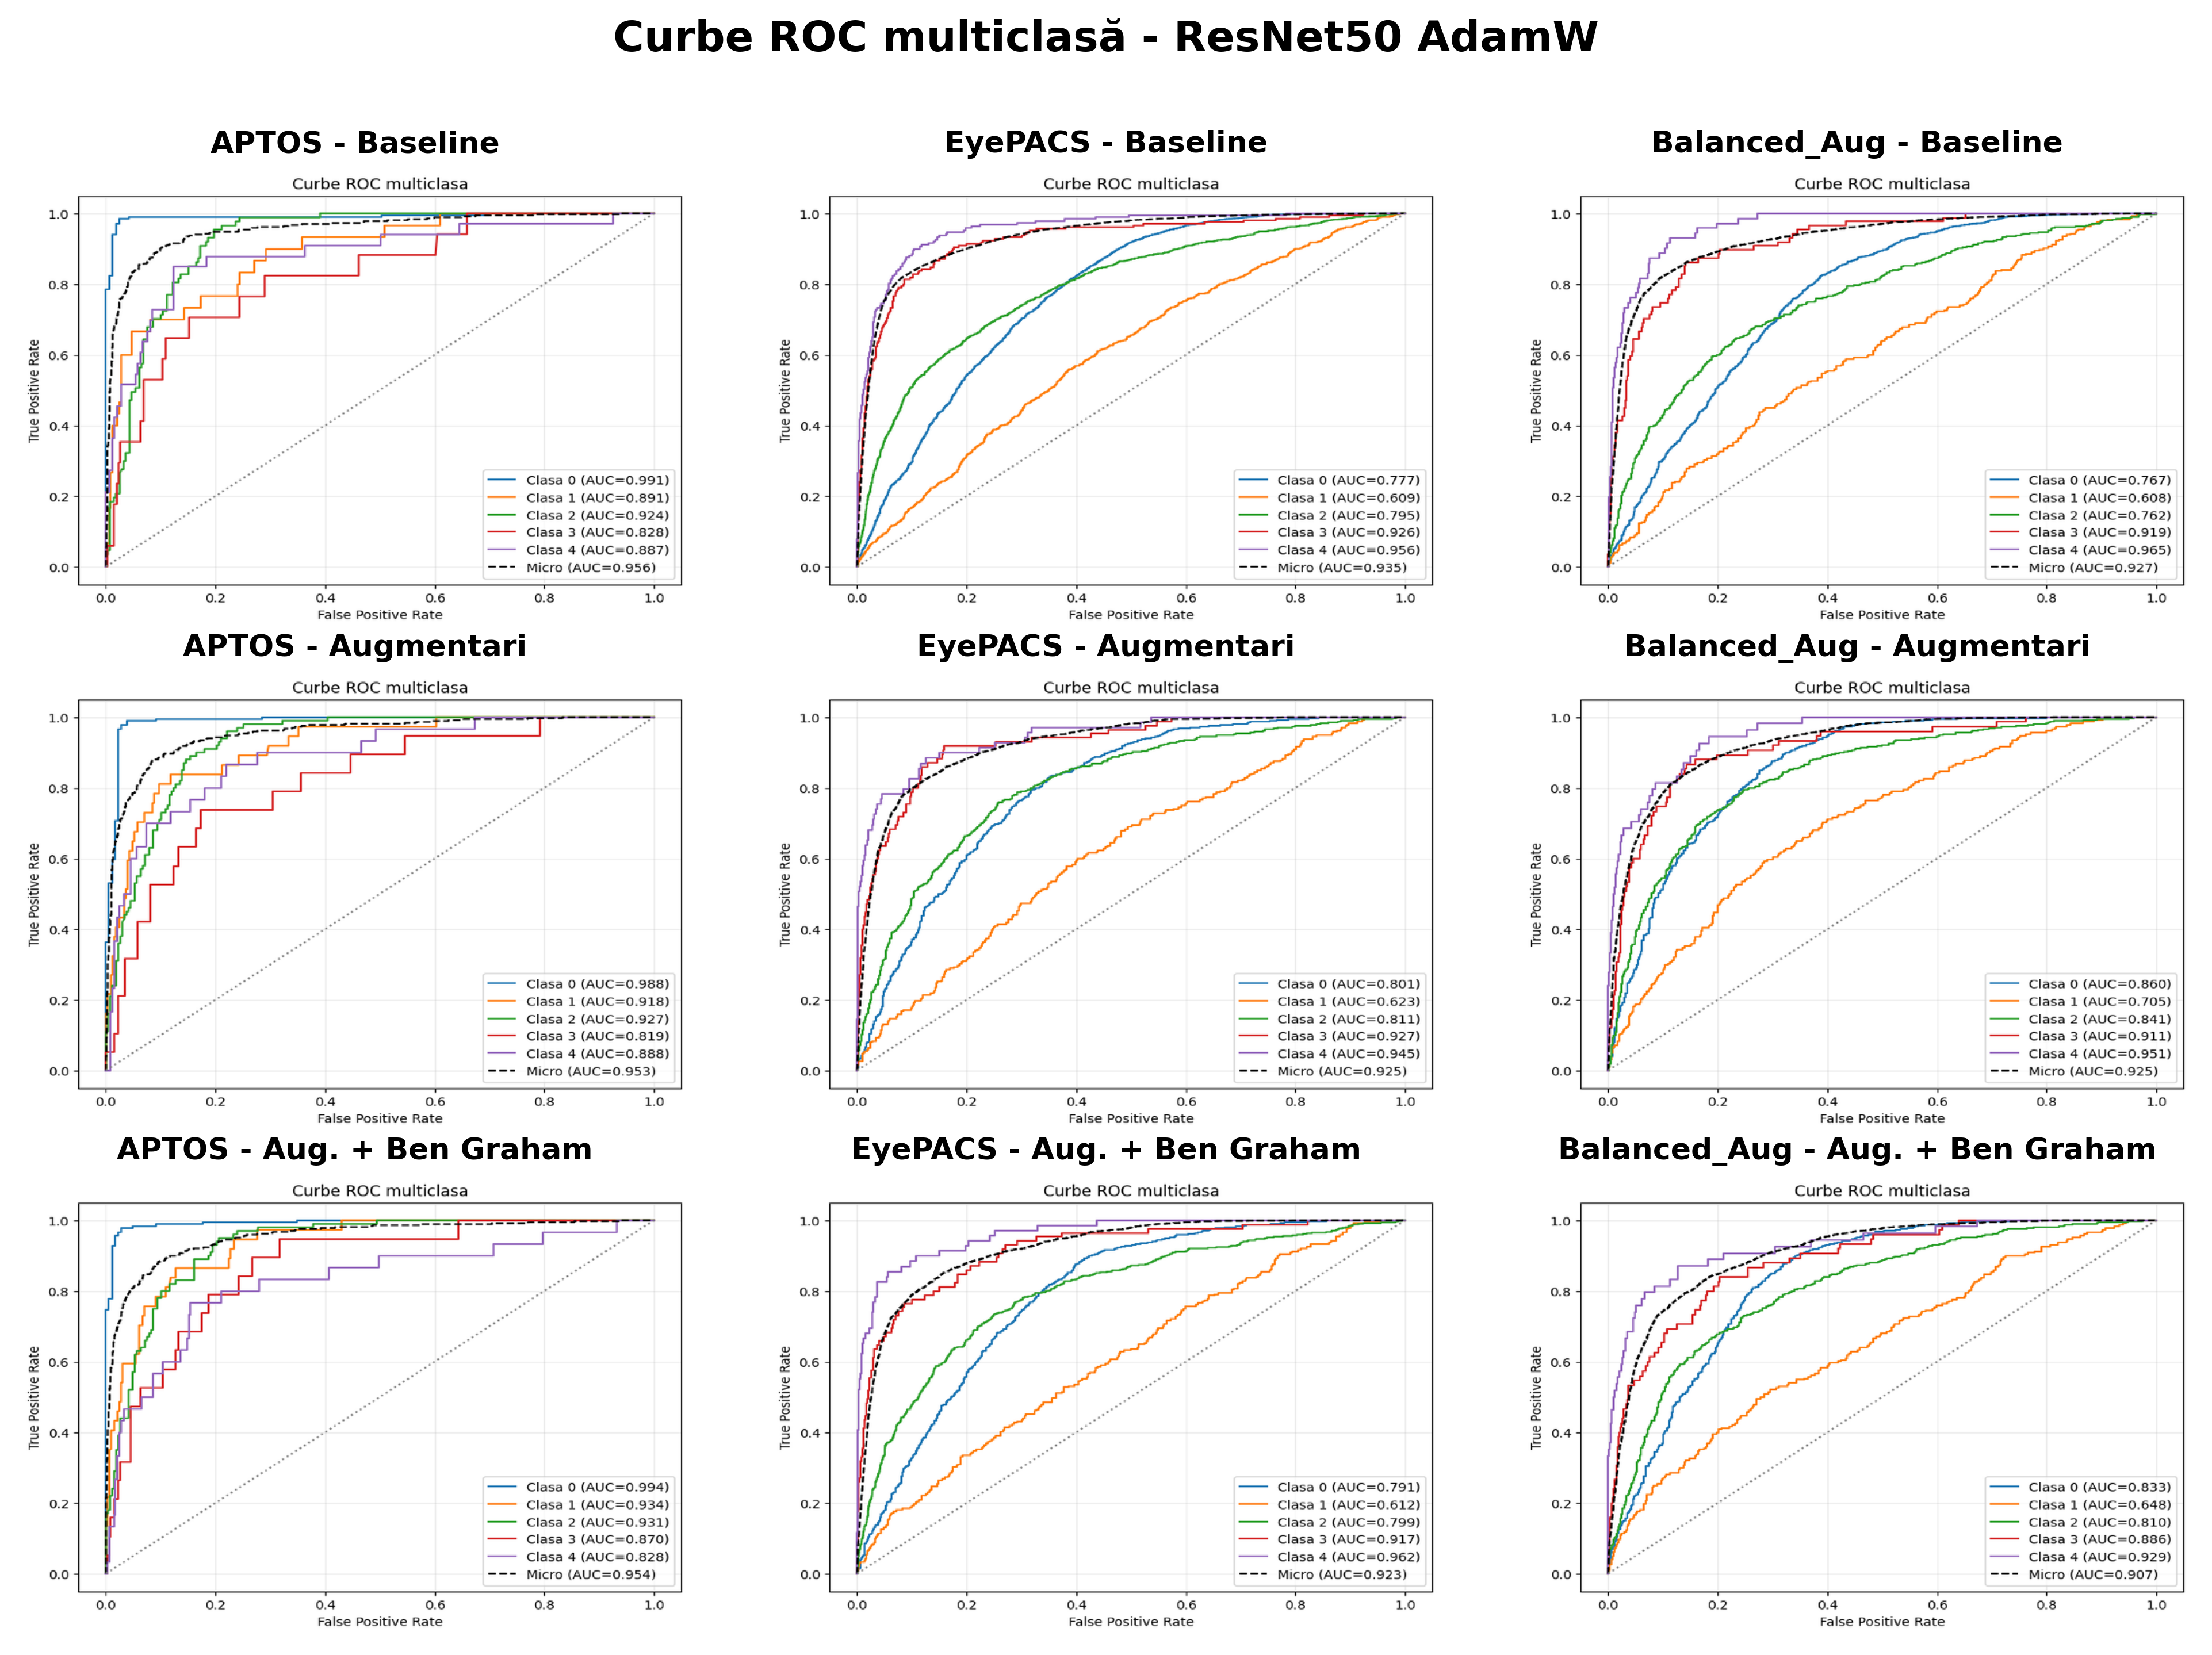
\includegraphics[width=0.98\textwidth]{Figuri/cap6_roc_grid.png}
    \captionsetup{justification=centering}
    \caption{Curbele ROC multiclasă pentru cele nouă experimente ResNet50 cu AdamW din \texttt{experiments.ipynb}.}
    \label{fig:cap6-roc-grid}
\end{figure}

\ \ \ \ Din figura \ref{fig:cap6-roc-grid} se observă că performanța nu trebuie interpretată doar prin
poziția generală a curbelor, ci și prin diferențele dintre clase. Curbele apropiate de colțul
stânga-sus indică o separare bună între clasa analizată și restul claselor, ceea ce sugerează că
modelul atribuie scoruri probabilistice mai sigure. În general, clasele extreme sunt mai ușor de
separat: imaginile fără retinopatie au aspect diferit față de imaginile patologice avansate, iar
clasele severe conțin leziuni mai vizibile. În schimb, clasele intermediare au curbe mai puțin
ideale, deoarece diferențele vizuale dintre formele ușoare și moderate sunt subtile și pot depinde
mult de iluminare, calitatea imaginii și preprocesare.
\bigskip

\ \ \ \ Comparativ cu matricele de confuzie, curbele ROC oferă o perspectivă mai fină asupra
încrederii modelului. O matrice de confuzie arată eticheta finală aleasă, în timp ce ROC arată dacă
modelul a acordat totuși scoruri rezonabile clasei corecte înainte de aplicarea pragului sau a
deciziei finale. Din acest motiv, o curbă ROC bună poate indica faptul că modelul are informație utilă
în scorurile sale, chiar dacă unele predicții finale rămân greșite. Această observație susține și
abordarea în două etape: prima etapă poate fi optimizată pentru separarea robustă între sănătos și
patologic, iar a doua etapă poate trata separat diferențele mai dificile dintre clasele 1--4.
\bigskip

\section{Integrarea cu sistemul final în două etape}

\ \ \ \ Varianta finală a experimentului este implementată în notebook-ul
\path{Notebooks/Main/Local/diabetic-retinopathy-classifier-FIXED-3ramuri.ipynb}, iar rezultatele
exportate sunt grupate în directorul \path{Notebooks/Main/Local/Rezultate_main}. Spre deosebire de
experimentele comparative anterioare, această rulare urmărește direct configurația folosită în
sistemul final: un model \texttt{EfficientNet-B3} pentru decizia binară sănătos--patologic și un al
doilea model \texttt{EfficientNet-B3} pentru gradarea severității pe clasele 1--4. Separarea celor două
sarcini reduce dificultatea problemei multiclasă, deoarece clasa sănătoasă nu mai concurează direct cu
stadiile patologice în același clasificator.
\bigskip

Prima etapă tratează problema ca o clasificare binară între imaginile \textit{sănătoase} și imaginile
cu retinopatie diabetică. Criteriul de selecție este AUC pe validare, deoarece în această etapă este
important ca modelul să ordoneze cât mai bine imaginile sănătoase față de cele patologice, înainte de
alegerea pragului final. În ultima rulare, cel mai bun AUC pe validare este \(0.8634\), iar pe setul de
test modelul obține un AUC de \(0.8567\). Pragul operațional este ales pe setul de validare prin
\(F_2\), ceea ce favorizează recall-ul pentru clasa patologică. La pragul \(0.099\), raportul de test
indică o acuratețe de \(0.763\), precision de \(0.743\) și recall de \(0.805\) pentru clasa
\textit{Bolnav}. Valoarea redusă a pragului nu urmărește maximizarea acurateții brute, ci reducerea
fals-negativelor, astfel încât imaginile suspecte să fie trimise mai departe către etapa de gradare.
\bigskip

A doua etapă este aplicată imaginilor trimise mai departe de modelul binar și clasifică severitatea în
stadiile 1--4. Pentru această etapă a fost păstrată formularea de tip \textit{regression}, deoarece
scorul continuu este transformat în clase prin praguri optimizate pe validare, iar metrica principală
devine Quadratic Weighted Kappa. Pragurile obținute pe validare sunt aproximativ \(0.580\), \(1.393\)
și \(2.158\). Modelul atinge un Val QWK de \(0.6575\), iar pe test obține accuracy \(0.6170\) și QWK
\(0.6576\). Scorurile macro pentru etapa de severitate sunt precision \(0.577\), recall \(0.597\) și
F1 \(0.572\), ceea ce confirmă că problema rămâne dificilă mai ales pentru stadiile intermediare.
\bigskip

\begin{figure}[H]
    \centering
    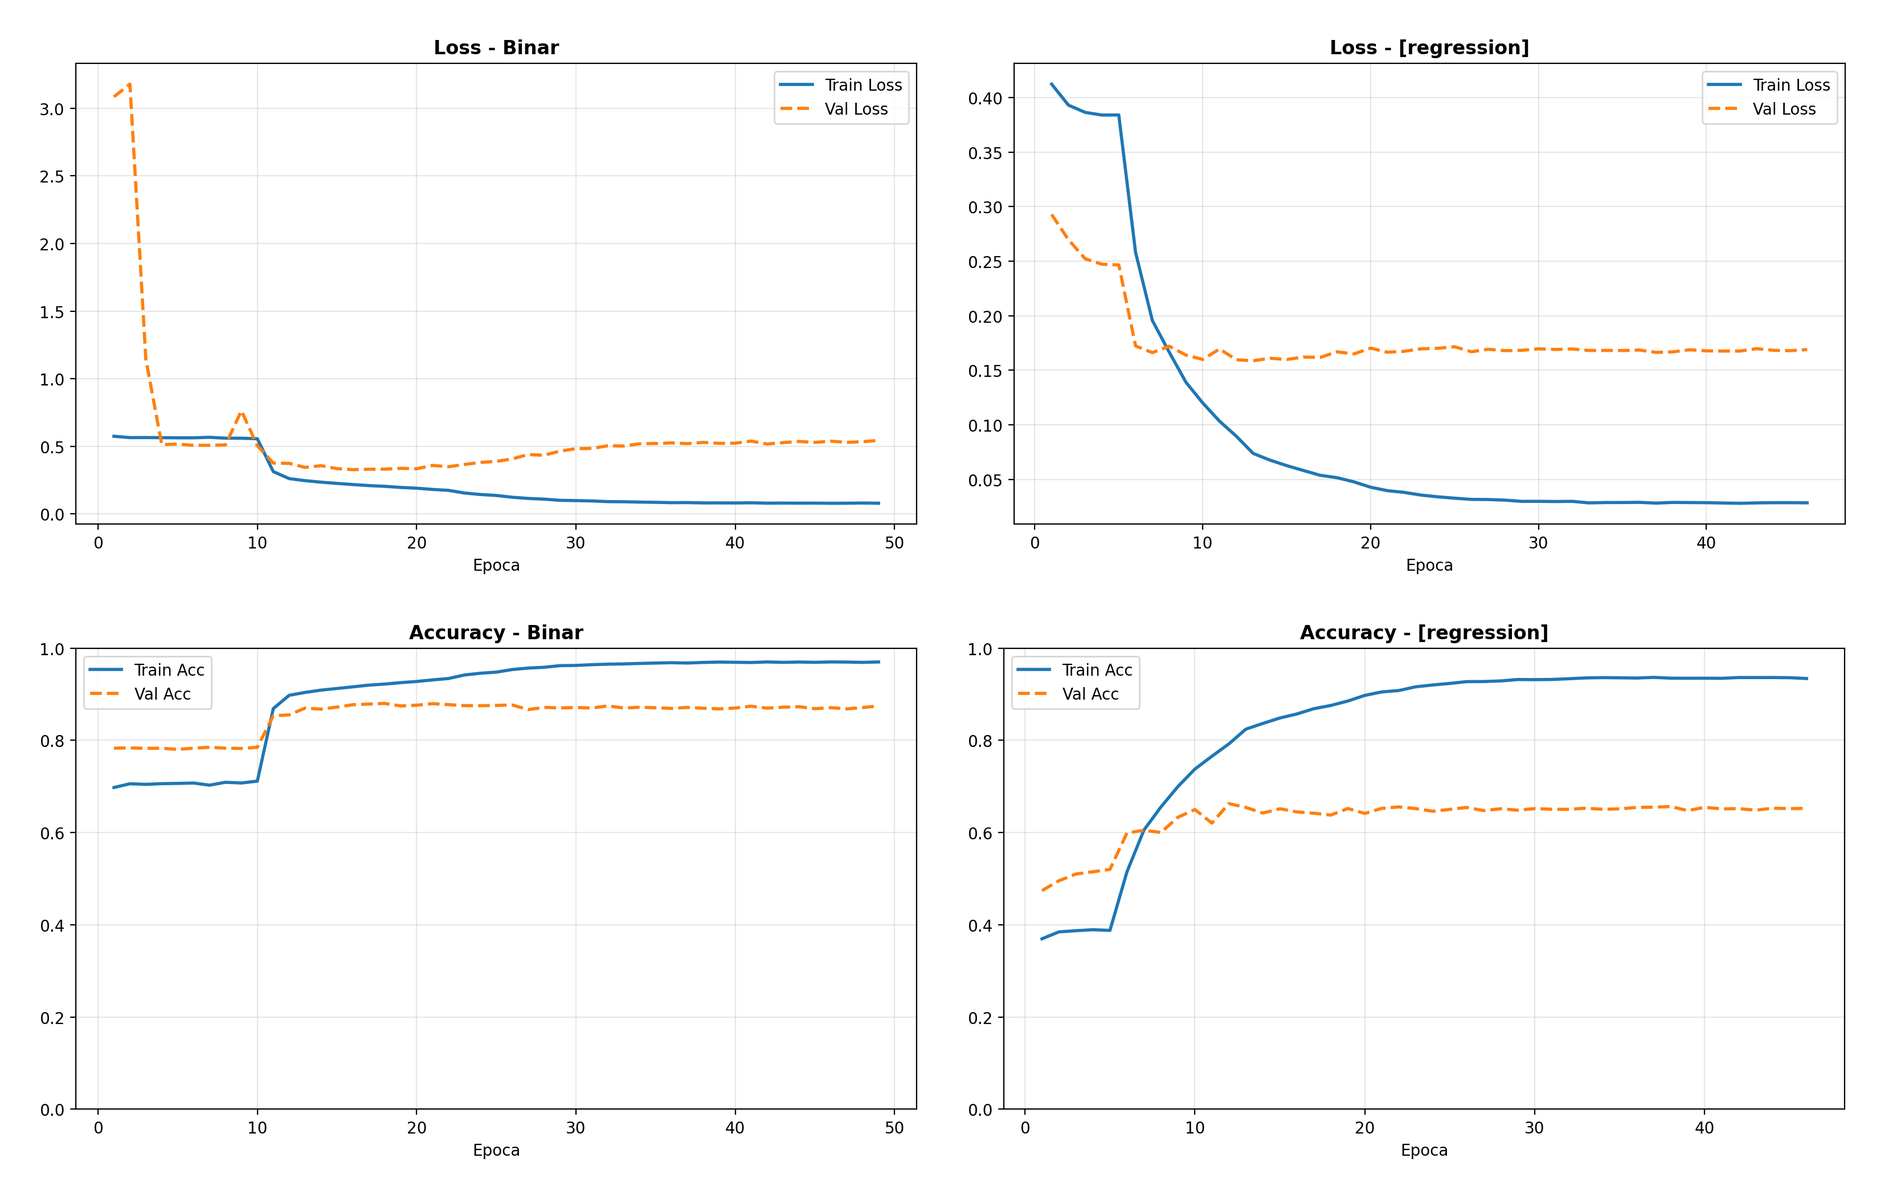
\includegraphics[width=0.98\textwidth]{Figuri/cap6_11_curbe_loss_acc_main.png}
    \captionsetup{justification=centering}
    \caption{Curbele de pierdere și acuratețe pentru detectorul binar și pentru modelul de severitate
    1--4 prin regresie.}
    \label{fig:cap6-11-curbe-loss-acc-main}
\end{figure}

\ \ \ \ Figura \ref{fig:cap6-11-curbe-loss-acc-main} reunește evoluția pierderii și a acurateții pentru
cele două componente ale sistemului final. Pentru detectorul binar, pierderea pe validare este cea care
scade brusc la început, după care se stabilizează și fluctuează în jurul unor valori mai mici. Pierderea
pe antrenare are o evoluție mai graduală, ceea ce indică faptul că modelul continuă să ajusteze
separarea dintre imaginile sănătoase și cele patologice. Acest comportament este frecvent în setările
de screening, unde imaginile din validare pot avea calitate, iluminare și leziuni diferite față de cele
din antrenare. De aceea, selecția modelului nu se bazează doar pe valoarea
pierderii, ci pe capacitatea scorurilor de a separa cele două clase.
\bigskip 

În partea de acuratețe, detectorul binar ajunge relativ repede într-o zonă stabilă pe validare.
Acuratețea rămâne însă o metrică secundară pentru această componentă, deoarece pragul final este ales
pentru a favoriza sensibilitatea față de cazurile patologice. Astfel, o acuratețe de test de \(0.763\)
trebuie interpretată împreună cu recall-ul de \(0.805\) pentru clasa \textit{Bolnav}: modelul acceptă o
parte dintre falsele pozitive pentru a reduce riscul ca o imagine cu retinopatie diabetică să fie
respinsă încă din prima etapă.
\bigskip

Pentru modelul de severitate, pierderea pe validare scade mai brusc decât pierderea pe antrenare și se
stabilizează relativ repede, în jurul epocilor 15--20. Pierderea pe antrenare continuă să scadă mai
mult timp și se stabilizează mai târziu, aproximativ în jurul epocii 30. Acest lucru arată că modelul
continuă să ajusteze reprezentările pe setul de antrenare chiar și după ce performanța pe validare a
ajuns într-o zonă stabilă. Acuratețea de validare se stabilizează în zona
\(0.64\)--\(0.66\), ceea ce indică faptul că modelul învață reprezentări utile, dar rămâne limitat de
suprapunerea vizuală dintre stadiile patologice. Diferența dintre stadiile 1 și 2 sau dintre stadiile 3
și 4 poate fi subtilă, iar imaginile pot conține semne locale care nu domină întreaga fotografie de fund
de ochi.
\bigskip

\begin{figure}[H]
    \centering
    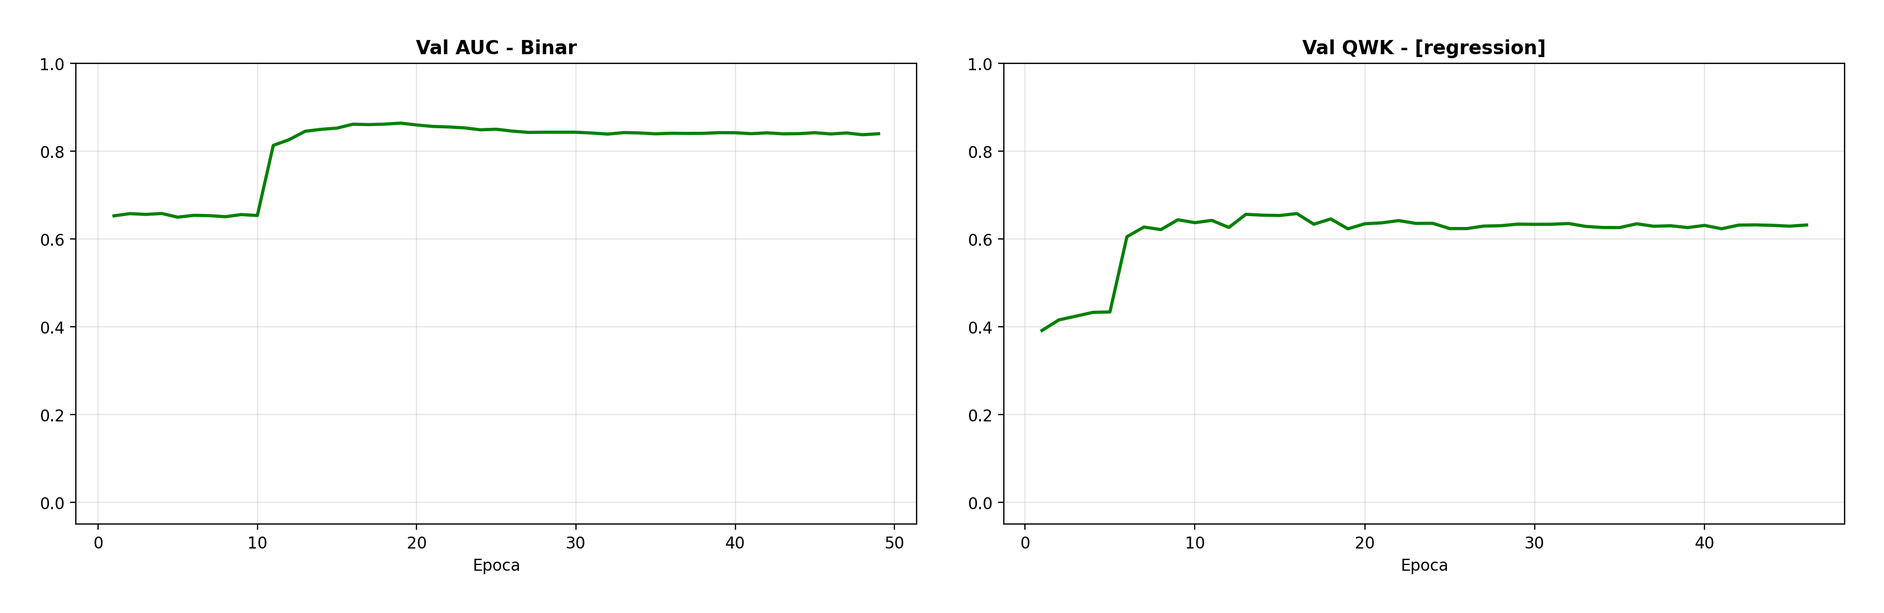
\includegraphics[width=0.98\textwidth]{Figuri/cap6_11_auc_qwk_main.png}
    \captionsetup{justification=centering}
    \caption{Evoluția AUC pentru detectorul binar și a QWK pentru modelul de severitate 1--4 prin
    regresie.}
    \label{fig:cap6-11-auc-qwk-main}
\end{figure}

\ \ \ \ Figura \ref{fig:cap6-11-auc-qwk-main} pune alături metricile principale de monitorizare pentru
cele două etape. Curba AUC este cea mai relevantă pentru detectorul binar, deoarece nu depinde de un
prag fix. Valoarea maximă de \(0.8634\) pe validare și valoarea de \(0.8567\) pe test arată că modelul
păstrează o capacitate bună de separare și în afara setului folosit pentru alegerea checkpoint-ului.
Diferența mică dintre validare și test sugerează că performanța nu este rezultatul unei ajustări
accidentale pe validare, deși valorile obținute arată și limitele problemei: există în continuare
imagini sănătoase cu aspect suspect și imagini patologice cu semne discrete, greu de separat automat.
\bigskip

Pentru etapa de severitate, QWK este mai informativă decât acuratețea simplă, deoarece ține cont de
ordinea clinică a claselor. Pe test, modelul obține accuracy \(0.6170\) și QWK \(0.6576\), ceea ce arată
că o parte dintre erori rămân între clase apropiate și nu reprezintă confuzii complet arbitrare. Această
interpretare este importantă în formularea prin regresie, unde scorul continuu este transformat în
clase prin praguri optimizate pe validare.
\bigskip

\begin{figure}[H]
    \centering
    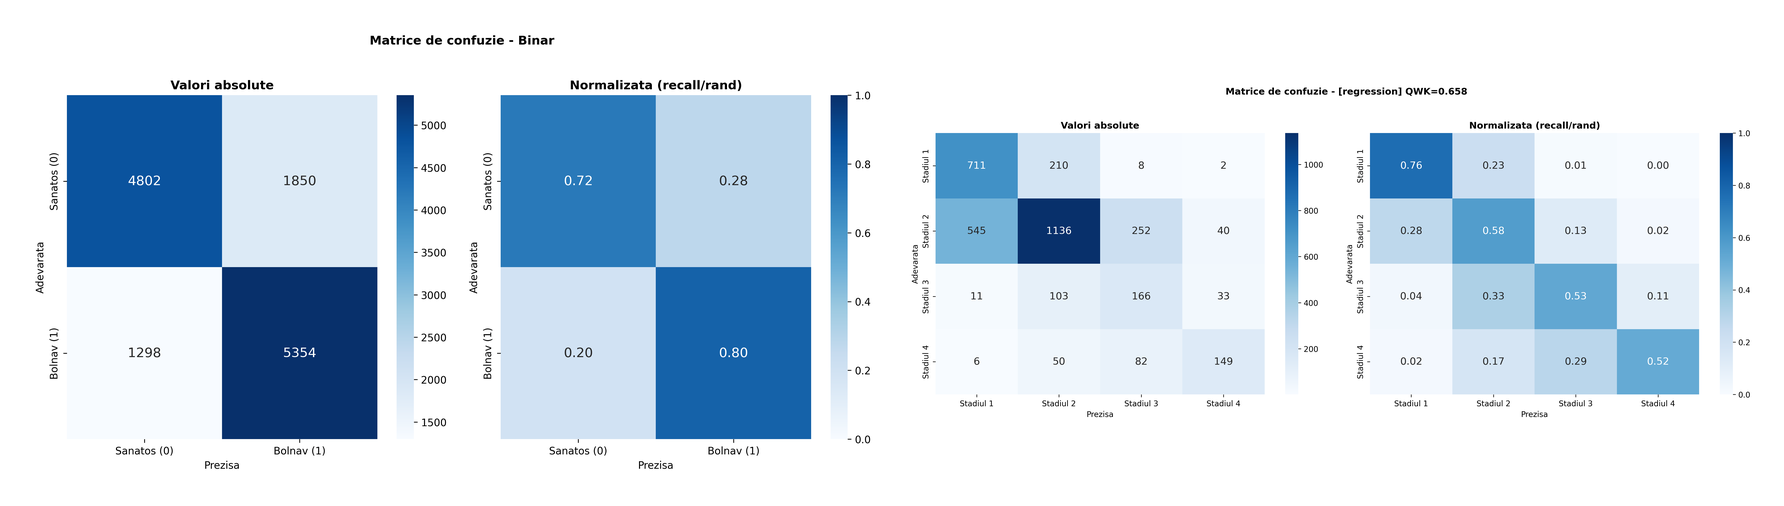
\includegraphics[width=0.98\textwidth]{Figuri/cap6_11_matrici_absolute_main.png}
    \captionsetup{justification=centering}
    \caption{Matrici de confuzie absolute pentru detectorul binar și pentru modelul de severitate
    1--4 prin regresie.}
    \label{fig:cap6-11-matrici-absolute-main}
\end{figure}

\ \ \ \ Matricile de confuzie din figura \ref{fig:cap6-11-matrici-absolute-main} evidențiază explicit
efectul pragului optimizat pentru screening. Modelul binar identifică \(5354\) imagini patologice din
\(6652\), ceea ce corespunde unui recall de aproximativ \(0.805\) pentru clasa \textit{Bolnav}. În
același timp, apar \(1850\) false pozitive, adică imagini sănătoase trimise mai departe către modelul
de severitate. Aceste cazuri nu pot fi corectate automat de etapa a doua, deoarece modelul de
severitate primește doar clase patologice și va atribui inevitabil o clasă din intervalul 1--4, de
obicei una joasă dacă imaginea seamănă mai mult cu un caz ușor. Prin urmare, pragul ales reprezintă un
compromis de screening: acceptă mai multe false pozitive pentru a reduce fals-negativele, deoarece un
fals negativ în etapa binară ar opri complet analiza unei imagini patologice.
\bigskip

Pentru etapa 1--4, cele mai multe predicții corecte apar pentru stadiile 1 și 2, unde există și cel mai
mare suport în test. Confuzia dintre stadiile 1 și 2 rămâne principala sursă de eroare, iar stadiile 3
și 4 sunt afectate de numărul mai redus de exemple și de proximitatea vizuală a leziunilor. În contextul
sistemului final, etapa de severitate trebuie interpretată împreună cu decizia binară: ea poate diferenția
gradele de boală pentru imaginile suspecte, dar nu mai are o clasă 0 prin care să respingă un caz sănătos
trimis greșit mai departe.
\bigskip

\begin{figure}[H]
    \centering
    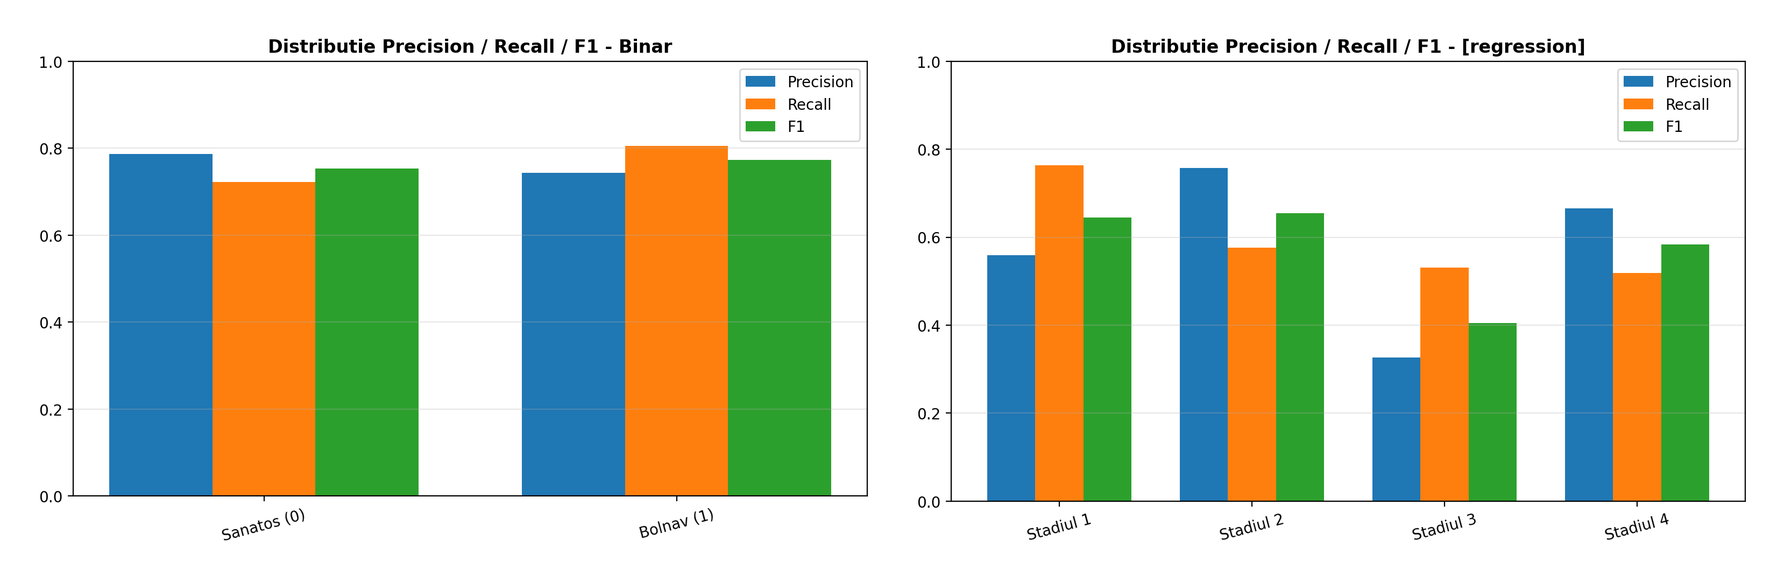
\includegraphics[width=0.98\textwidth]{Figuri/cap6_11_prf_main.png}
    \captionsetup{justification=centering}
    \caption{Distribuția indicatorilor precision, recall și F1 pentru detectorul binar și pentru
    modelul de severitate 1--4 prin regresie.}
    \label{fig:cap6-11-prf-main}
\end{figure}

\ \ \ \ Distribuția precision--recall--F1 din figura \ref{fig:cap6-11-prf-main} completează interpretarea
matricilor de confuzie. Pentru clasa patologică din detectorul binar, recall-ul este mai mare decât
precision-ul, ceea ce confirmă efectul pragului ales prin \(F_2\). Pentru clasa sănătoasă, scorurile
rămân apropiate, dar sunt influențate de falsele pozitive introduse deliberat de pragul scăzut. În
ansamblu, modelul binar nu este optimizat pentru o decizie izolată de diagnostic, ci pentru prima
filtrare a pipeline-ului: să separe suficient de bine imaginile fără boală de cele care trebuie
analizate mai detaliat.
\bigskip

Pentru etapa de severitate, indicatorii arată un comportament neuniform între clase. Clasa
\textit{Stadiul 2} are precision ridicat, dar recall mai redus, deoarece o parte dintre imaginile reale
de stadiu 2 sunt absorbite de stadiul 1. Clasa \textit{Stadiul 3} rămâne cea mai dificilă, cu F1 de
aproximativ \(0.404\), în timp ce stadiile extreme au un comportament mai stabil. Această distribuție
confirmă că dificultatea principală a etapei a doua nu este detectarea bolii, ci delimitarea exactă a
severității.
\bigskip

\ \ \ \ Integrarea finală se bazează, așadar, pe o decizie secvențială. Imaginea este preprocesată și
trimisă mai întâi către modelul binar. Dacă probabilitatea de boală este sub pragul stabilit pe
validare, sistemul returnează clasa 0. Dacă probabilitatea depășește pragul, imaginea este transmisă
către modelul de severitate, iar predicția este mapată în scala 1--4. Această arhitectură permite
optimizarea separată a sensibilității pentru screening și a respectării ordinii clinice pentru
stadiile patologice.
\bigskip

\section{Analiza calitativă a exemplelor de inferență}

\ \ \ \ Înainte de interpretarea exemplelor, este important de precizat cum este calculată valoarea afișată
în aplicația de inferență ca nivel de încredere, deoarece semnificația ei depinde de modelul selectat.
Pentru modelele experimentale multiclasă, rețeaua produce cinci scoruri, câte unul pentru fiecare clasă
0--4. Aceste scoruri sunt transformate în probabilități prin funcția \textit{softmax},
iar clasa finală este clasa cu probabilitatea maximă:
\[
p_i = \frac{e^{z_i}}{\sum_{j=0}^{4} e^{z_j}}, \qquad
\hat{y} = \arg\max_i p_i.
\]
În acest caz, valoarea afișată în interfață este probabilitatea softmax a clasei prezise, iar a doua
opțiune este următoarea clasă cu probabilitate mare.
\bigskip

Pentru pipeline-ul principal, valoarea afișată este calculată diferit, deoarece decizia este secvențială.
Prima etapă este detectorul binar, care produce un scor transformat prin sigmoid în probabilitatea de
boală:
\[
p_{\text{boală}} = \sigma(z), \qquad p_{\text{sănătos}} = 1 - p_{\text{boală}}.
\]
Dacă detectorul decide clasa 0, aplicația afișează ca nivel de încredere valoarea
\(p_{\text{sănătos}}\). Dacă imaginea este trimisă către etapa a doua, modelul de severitate folosit în
pipeline-ul principal produce un scor de regresie pentru clasele 1--4. Clasa este obținută prin
compararea scorului cu pragurile salvate în \texttt{rounder\_coef.npy}, iar nivelul de încredere afișat
este o estimare derivată din apropierea scorului față de cele patru grade:
\[
q_k = \frac{e^{-(k-s)^2}}{\sum_{r=0}^{3} e^{-(r-s)^2}}, \qquad k \in \{0,1,2,3\},
\]
unde \(s\) este scorul de regresie, iar \(q_k\) este apoi asociat claselor patologice 1--4. Prin urmare,
pentru pipeline-ul principal, procentul afișat la etapa de severitate nu este o probabilitate softmax
obținută direct din rețea, ci o estimare construită din scorul de regresie. În cardul \textit{Metadate
model} din aplicație, lista de probabilități afișată pentru clasele 1--4 este ponderată și cu
probabilitatea de boală a detectorului binar, pentru a reflecta întregul traseu al pipeline-ului.
\bigskip

\ \ \ \ Pentru a completa evaluarea cantitativă, au fost analizate și câteva exemple calitative generate prin
aplicația de inferență. Aceste exemple sunt utile deoarece arată nu doar clasa finală, ci și distribuția
scorurilor între clasele vecine, respectiv situațiile în care modelul este sigur sau ambiguu. În
continuare sunt prezentate patru cazuri reprezentative: trei rulări ale pipeline-ului principal și o
rulare a unui model experimental multiclasă.
\bigskip

\begin{figure}[H]
    \centering
    \captionsetup{justification=centering}
    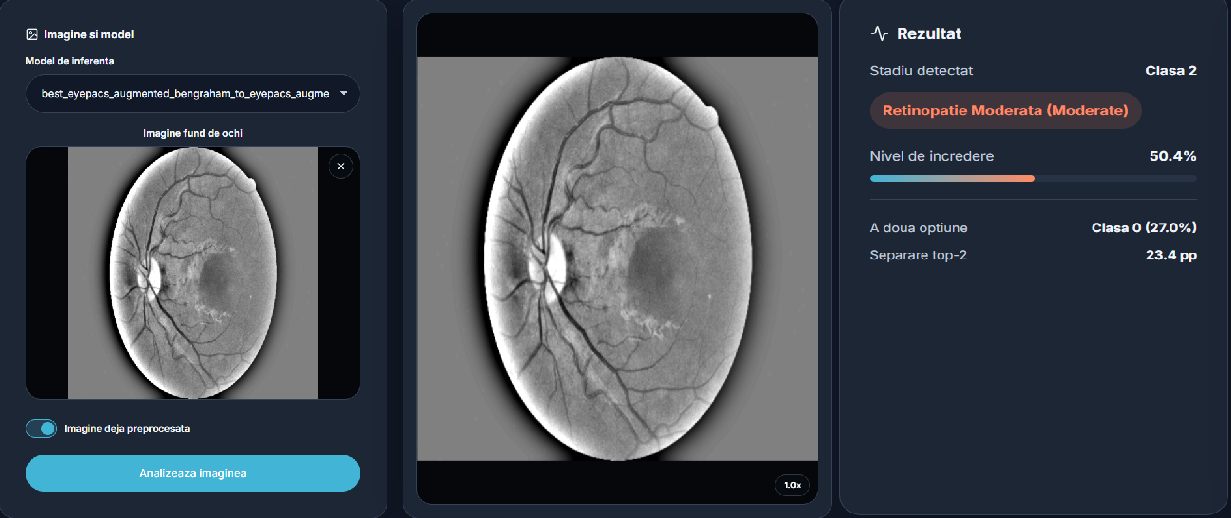
\includegraphics[width=0.95\textwidth]{Figuri/comentat_fig_model_exp_clasa2_fake0.png}
    \caption{Model experimental: imagine de clasa 2, cu al doilea scor ca mărime la clasa 0.}
    \label{fig:cap6-11-exp-fake0}
\end{figure} 

\ \ \ \ Exemplul din figura \ref{fig:cap6-11-exp-fake0} arată o limită importantă a clasificatoarelor
multiclasă antrenate direct pe toate clasele: deși imaginea aparține clasei 2, următorul scor ca mărime
este atribuit clasei 0. Predicția principală rămâne astfel corectă, dar distribuția scorurilor arată că
modelul păstrează o incertitudine importantă între un caz moderat și absența bolii. Această apropiere
este relevantă deoarece o mică modificare a scorurilor sau o imagine cu o calitate mai slabă ar putea
împinge decizia către clasa 0, generând un fals negativ. Exemplul evidențiază de ce un clasificator
multiclasă direct poate confunda uneori trăsăturile moderate cu aspectul normal al fundului de ochi și
de ce este utilă separarea explicită dintre detecția bolii și gradarea severității.
\bigskip 

\begin{figure}[H]
    \centering
    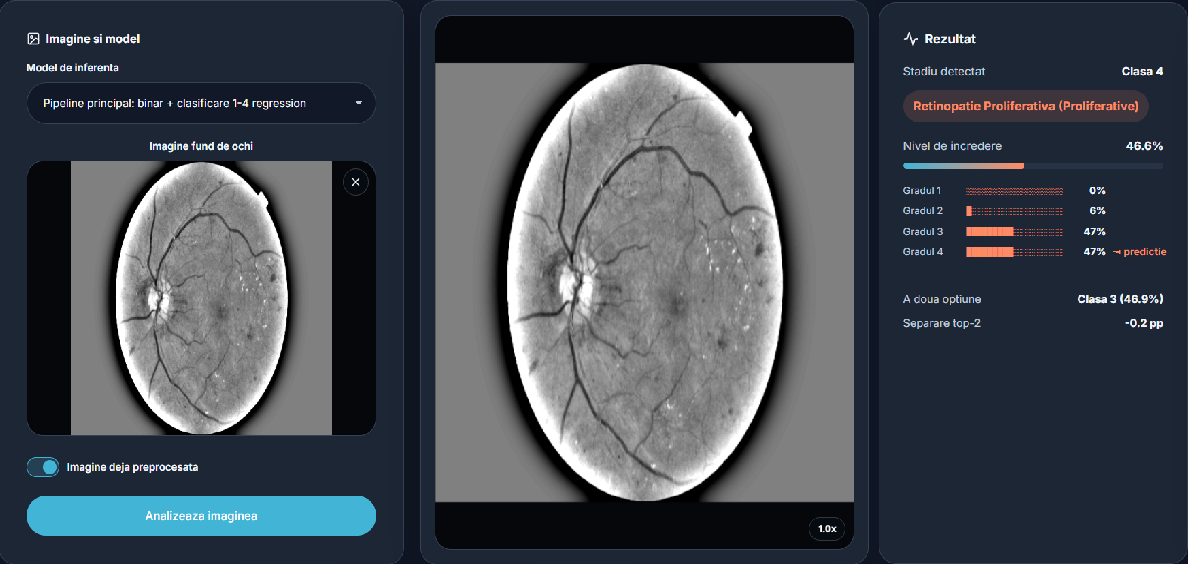
\includegraphics[width=0.95\textwidth]{Figuri/comentat_fig_model_principal_clasa4_but3.png}
    \caption{Pipeline principal: caz sever, cu scoruri apropiate între stadiile 3 și 4.}
    \label{fig:cap6-11-main-clasa4-but3}
\end{figure}

\ \ \ \ Figura \ref{fig:cap6-11-main-clasa4-but3} arată o limită a sistemului final: în cazurile severe,
scorurile pentru stadiile 3 și 4 pot fi foarte apropiate. Această ambiguitate este așteptată, deoarece
trecerea dintre retinopatia severă și cea proliferativă depinde de semne vizuale fine, de calitatea
imaginii și de prezența unor leziuni care pot fi localizate doar într-o regiune redusă a fundului de
ochi. Totuși, confuzia rămâne între clase vecine și nu schimbă concluzia principală că imaginea este
patologică și necesită evaluare medicală. Modelul semnalează corect severitatea ridicată, chiar dacă
granularitatea exactă între stadiile 3 și 4 rămâne dificilă.
\bigskip

\begin{figure}[H]
    \centering
    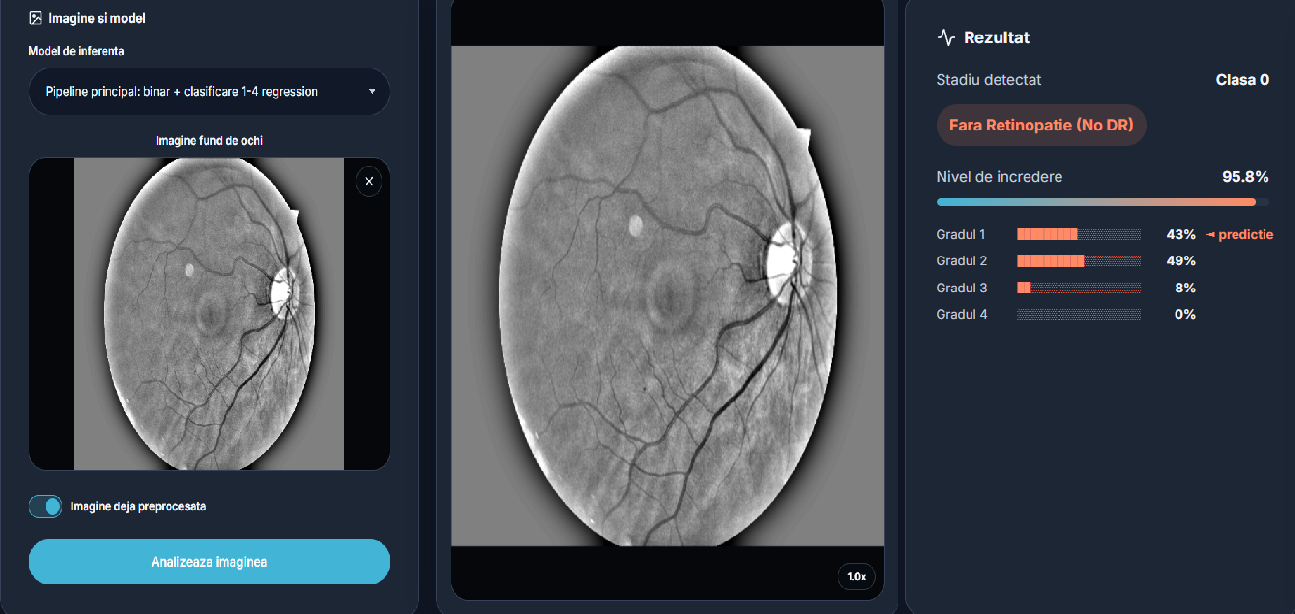
\includegraphics[width=0.95\textwidth]{Figuri/comentat_fig_model_principal_clasa0.png}
    \caption{Pipeline principal: decizie binară corectă pentru clasa 0.}
    \label{fig:cap6-11-main-clasa0}
\end{figure}

\ \ \ \ Exemplul din figura \ref{fig:cap6-11-main-clasa0} evidențiază avantajul sistemului principal.
Pentru imaginea normală, detectorul binar returnează clasa 0 cu încredere ridicată, iar distribuția
estimată pentru gradele 1--4 rămâne doar o informație secundară a clasificatorului de severitate.
Decizia finală nu este
lăsată să fie dominată de o confuzie între grade patologice, deoarece prima etapă filtrează cazul ca
nepatologic. Acesta este exact rolul sistemului în două etape: separarea robustă a imaginilor sănătoase
înainte de problema mai dificilă a gradării.
\bigskip   

\begin{figure}[H]
    \centering
    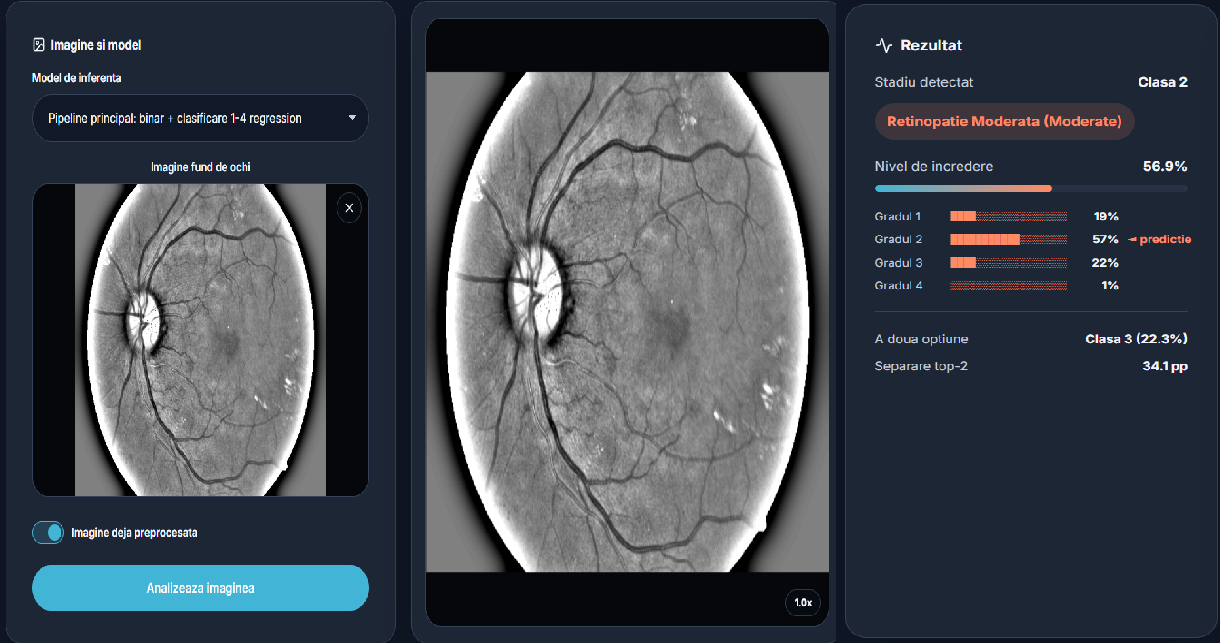
\includegraphics[width=0.95\textwidth]{Figuri/comentat_fig_model_principal_clasa2_true.png}
    \caption{Pipeline principal: exemplu patologic încadrat în stadiul 2.}
    \label{fig:cap6-11-main-clasa2-true}
\end{figure}

\ \ \ \ În figura \ref{fig:cap6-11-main-clasa2-true}, modelul principal indică un maxim clar pe gradul 2,
iar următoarea opțiune este gradul 3, adică o clasă vecină. Acest comportament este util clinic,
deoarece sistemul identifică imaginea ca patologică și păstrează incertitudinea în interiorul
stadiilor apropiate. O astfel de eroare potențială este mai acceptabilă decât o confuzie între sănătos
și boală, deoarece păstrează ordinea clinică a severității. Din acest motiv, sistemul în două etape este
preferabil unui singur clasificator cu cinci clase: prima etapă optimizează detecția bolii și reduce
fals-negativele, iar a doua etapă se concentrează pe gradarea cazurilor deja suspecte, unde erorile pot
fi interpretate în termeni de severitate ordinală.
\bigskip

\chapter{Aplicația de inferență}

\section{Scopul aplicației dezvoltate}

\ \ \ \ Pentru a demonstra utilizarea practică a modelelor antrenate, a fost dezvoltată o
aplicație web de inferență. Scopul aplicației este de a permite încărcarea unei
imagini de fund de ochi, selectarea unui model salvat sau a pipeline-ului principal și obținerea unei
predicții privind stadiul retinopatiei diabetice. Aplicația are rol experimental și nu înlocuiește
diagnosticul medical, deoarece sistemele automate pentru retinopatia diabetică necesită validare
clinică riguroasă înainte de utilizare în screening sau decizie medicală \cite{3_gulshan2016development},
\cite{15_li2019diagnostic}.
\bigskip

Rezultatul afișat include clasa prezisă, denumirea stadiului, nivelul de încredere, a doua opțiune
atunci când aceasta poate fi calculată, separarea dintre primele două clase, timpul de execuție și
recomandări orientative pentru medic și pacient. Interfața include și metadate tehnice păstrate la
nivelul informațiilor utile pentru interpretare: fișierul folosit, arhitectura, dimensiunea de intrare,
dimensiunea imaginii originale, dimensiunea imaginii folosite efectiv la inferență, metoda de
preprocesare și, pentru pipeline-ul principal, detectorul binar, modelul de severitate și ramura
utilizată.

\section{Arhitectura aplicației}

\ \ \ \ Aplicația este organizată în două componente principale: un backend Flask și un
frontend React, două tehnologii potrivite pentru separarea logicii de inferență de interfața
utilizatorului \cite{flask_docs}, \cite{react_docs}. Backend-ul este responsabil pentru încărcarea modelului, verificarea și preprocesarea imaginii,
precum și calcularea predicției. Frontend-ul este responsabil pentru interfața de utilizare,
selecția modelului, încărcarea imaginii, vizualizarea imaginii preprocesate și afișarea rezultatului.
\bigskip

Cele două componente comunică prin cereri HTTP. Backend-ul expune endpoint-uri sub forma
\texttt{/api/models} și \texttt{/api/predict}, iar frontend-ul trimite cereri către acestea folosind biblioteca Axios
\cite{axios_docs}. Pentru comunicarea între porturi diferite, backend-ul folosește
\texttt{flask\_cors}, care permite configurarea politicilor CORS pentru aplicații Flask
\cite{flask_cors_docs}. Endpoint-ul \texttt{/api/models} returnează atât lista modelelor, cât și
grupurile folosite în selectorul din interfață, iar endpoint-ul \texttt{/api/predict} primește imaginea,
identificatorul modelului și opțiunea prin care utilizatorul precizează dacă imaginea este deja
preprocesată.

\section{Componenta backend}

\ \ \ \ Componenta backend este implementată în fișierul \texttt{Inference\_site/app.py}. Aceasta definește aplicația Flask, stabilește
directorul în care se află modelele salvate și selectează dispozitivul de calcul:
CUDA, dacă este disponibil, sau CPU în caz contrar. Pentru reconstruirea arhitecturii
modelului, backend-ul importă funcția \texttt{get\_model} din \texttt{builder.py}.
\bigskip

Endpoint-ul \texttt{/api/models} returnează un catalog de modele, nu doar o listă simplă de fișiere.
Catalogul este împărțit în două grupuri: \textit{Modele principale}, care conține pipeline-ul final
\texttt{binar + clasificare 1--4 regression}, și \textit{Experimente}, care conține modelele salvate în
directorul \path{Notebooks/Rezultate/New/modele}. Pentru soluția principală sunt folosite ponderile
detectorului binar din
\path{Notebooks/Main/Local/Rezultate_main/binar/efficientnet_b3_binar_best.pth} și ponderile modelului
de severitate din \path{Notebooks/Main/Local/Rezultate_main/clasificare_regression/model_best.pth},
împreună cu pragurile de rotunjire salvate în \texttt{rounder\_coef.npy}. Dacă unul dintre aceste fișiere
lipsește, opțiunea principală este păstrată în catalog, dar este marcată ca indisponibilă.
\bigskip

Endpoint-ul \texttt{/api/predict} primește imaginea, identificatorul modelului selectat și câmpul
\texttt{image\_preprocessed}. Dacă utilizatorul marchează imaginea ca fiind deja preprocesată, backend-ul
o folosește direct pentru inferență și reține acest lucru în răspunsul JSON. În caz contrar, imaginea
este convertită în RGB și trecută printr-o preprocesare de tip Ben Graham cu mască de retină, la
rezoluția \(512 \times 512\). Imaginea finală este apoi redimensionată la dimensiunea așteptată de
model: \(300 \times 300\) pentru pipeline-ul principal EfficientNet-B3, respectiv \(224 \times 224\) sau
\(299 \times 299\) pentru modelele experimentale, în funcție de arhitectură. Tensorul rezultat este
normalizat cu valorile ImageNet, iar predicția este calculată cu \texttt{torch.no\_grad()}, pentru a
dezactiva calculul gradientului în timpul inferenței \cite{pytorch_docs}.
\bigskip

Pentru opțiunea principală, backend-ul rulează o decizie secvențială. Prima etapă încarcă detectorul
binar \texttt{EfficientNet-B3} și calculează probabilitatea ca imaginea să fie patologică. Dacă această
probabilitate nu depășește pragul operațional al aplicației, sistemul returnează clasa 0. Dacă imaginea
este considerată patologică, rezultatul final este dat de modelul de regresie pentru clasele 1--4:
scorul continuu este mapat prin pragurile învățate pe validare, iar clasa rezultată este translatată în
scala finală 1--4. În implementarea curentă, etapa a doua este evaluată și pentru a putea furniza
metadate despre scorul de severitate, însă predicția finală folosește ramura 1--4 doar atunci când
detectorul binar trece pragul. Răspunsul JSON include detectorul folosit, modelul de etapă a doua,
probabilitatea de boală, scorul de regresie și detaliile de preprocesare.

\section{Componenta frontend}

\ \ \ \ Componenta frontend este implementată în \texttt{Inference\_site/App.jsx}. La pornire, aceasta solicită catalogul de
modele disponibile și selectează automat prima opțiune validă. Selectorul este organizat pe grupuri,
astfel încât utilizatorul poate alege între pipeline-ul principal și modelele experimentale din
directorul de rezultate. În versiunea actuală, opțiunea principală este afișată explicit ca
\texttt{Pipeline principal: binar + clasificare 1-4 regression}, iar modelele experimentale sunt
listate separat, cu numele fișierelor \texttt{.pth} generate în etapa de antrenare. Dacă pipeline-ul
principal nu poate fi încărcat din cauza unui fișier lipsă, opțiunea apare ca indisponibilă în selector.
\bigskip

După alegerea modelului, utilizatorul poate încărca imaginea prin apăsare sau drag-and-drop. Interfața
afișează previzualizarea imaginii originale și oferă un comutator numit \textit{Imagine deja
preprocesată}. Acest comutator controlează dacă backend-ul aplică sau nu preprocesarea Ben Graham
înainte de inferență. În partea dreaptă, aplicația afișează imaginea folosită efectiv de model; aceasta
poate fi mărită cu rotița mouse-ului, deplasată prin drag și resetată prin dublu click. Pentru
compararea ergonomiei vizuale, aplicația include și un comutator pentru modul light/dark.

\begin{figure}[H]
\centering
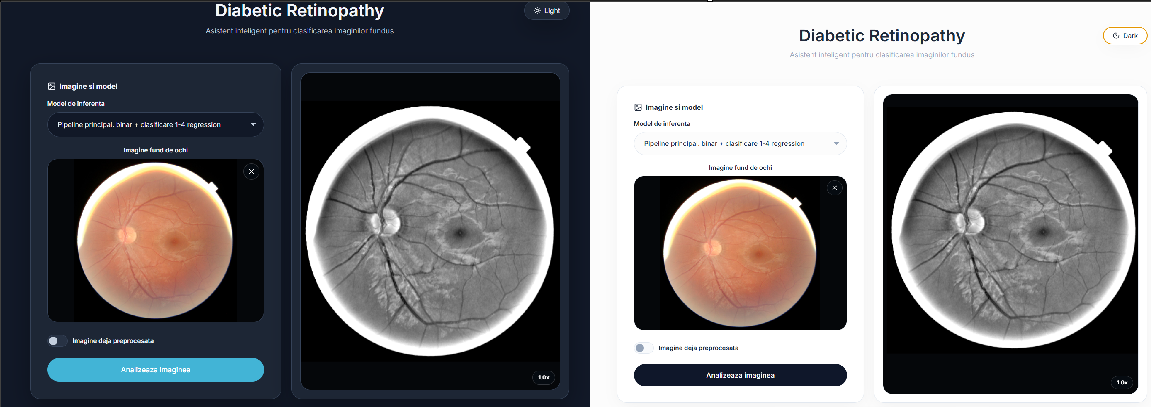
\includegraphics[width=0.95\textwidth]{Figuri/web_inference_interface.png}
\captionsetup{justification=centering}
\caption{Interfața aplicației de inferență în modurile dark și light, cu selectorul de model, previzualizarea imaginii și imaginea folosită la inferență}
\label{fig:app-frontend}
\end{figure}

\ \ \ \ După apăsarea butonului de analiză, frontend-ul construiește un obiect \texttt{FormData} care
conține imaginea, identificatorul modelului și starea comutatorului de preprocesare. Răspunsul primit
de la backend este afișat în trei carduri: rezultatul, recomandările și metadatele modelului. Cardul de
rezultat conține clasa detectată, denumirea clinică a stadiului, nivelul de încredere, a doua opțiune
și diferența procentuală dintre primele două opțiuni atunci când acestea sunt disponibile. Pentru
pipeline-ul principal, cardul poate afișa și distribuția estimată pe gradele 1--4, derivată din scorul
de regresie. Cardul de recomandări separă mesajul pentru medic de mesajul pentru pacient și include o
observație tehnică despre aplicarea preprocesării. Cardul de metadate arată probabilitățile sau
scorurile pipeline-ului, fișierele folosite, arhitectura, dimensiunile imaginilor, timpul de execuție,
metoda de preprocesare și ramura de clasificare.

\begin{figure}[H]
\centering
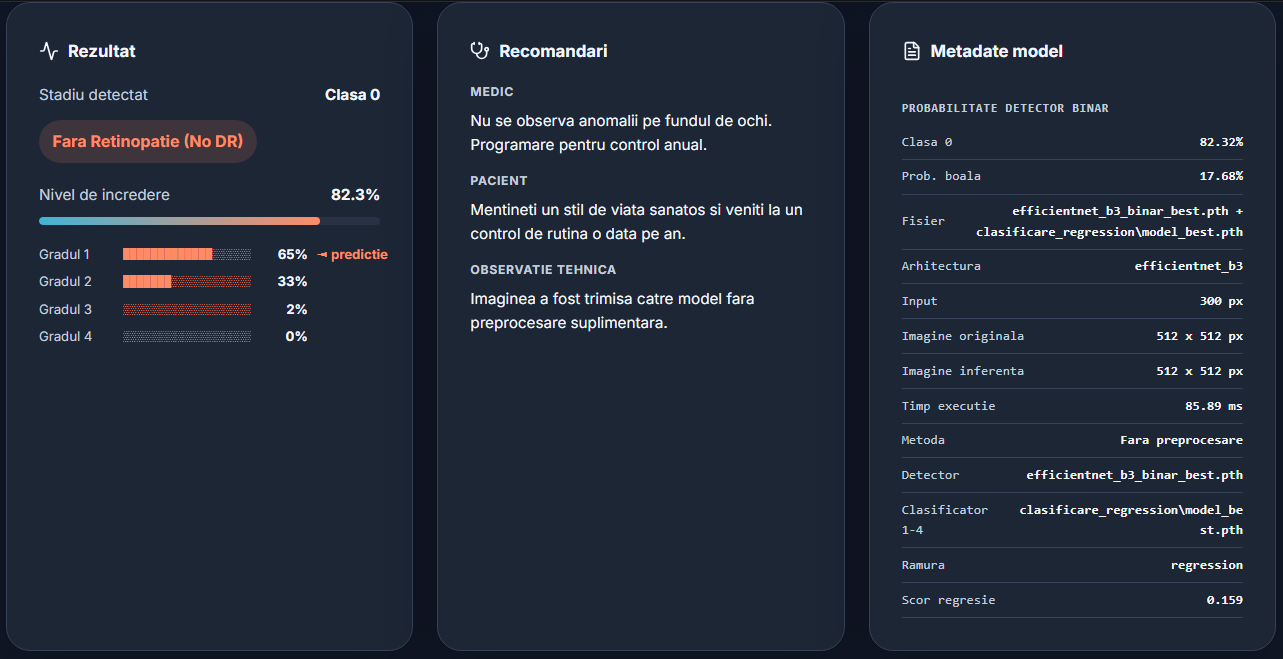
\includegraphics[width=0.95\textwidth]{Figuri/recommendations_website.png}
\captionsetup{justification=centering}
\caption{Cardurile de rezultat, recomandări și metadate tehnice afișate după rularea pipeline-ului principal}
\label{fig:recommendations-website}
\end{figure}

\section{Fluxul de utilizare}

\ \ \ \ Fluxul de utilizare este simplu. Utilizatorul pornește backend-ul, deschide frontend-ul, selectează modelul
dorit, încarcă o imagine de fund de ochi, stabilește dacă imaginea este deja preprocesată și apasă
butonul de analiză. Imaginea este trimisă către server, unde este analizată conform opțiunii selectate.
Rezultatul este apoi returnat în format JSON și afișat în interfața web.
\bigskip

Această structură permite testarea rapidă a mai multor modele pe aceeași imagine.
De exemplu, o imagine poate fi analizată mai întâi cu pipeline-ul principal în două etape, apoi cu
modele experimentale ResNet50, EfficientNet-B3, InceptionV3 sau Inception-ResNet-V2. Diferențele
dintre scoruri pot oferi indicii despre stabilitatea predicției și despre sensibilitatea arhitecturilor
la aceeași intrare. Compararea trebuie însă făcută cu prudență, deoarece modelele experimentale
afișează probabilități softmax multiclasă, în timp ce pipeline-ul principal combină probabilitatea
detectorului binar cu o estimare derivată din scorul de regresie al modelului 1--4. Selectorul de
modele păstrează modelele principale separate de experimente, astfel încât scenariul final al lucrării
rămâne ușor de identificat.

\begin{figure}[H]
\centering
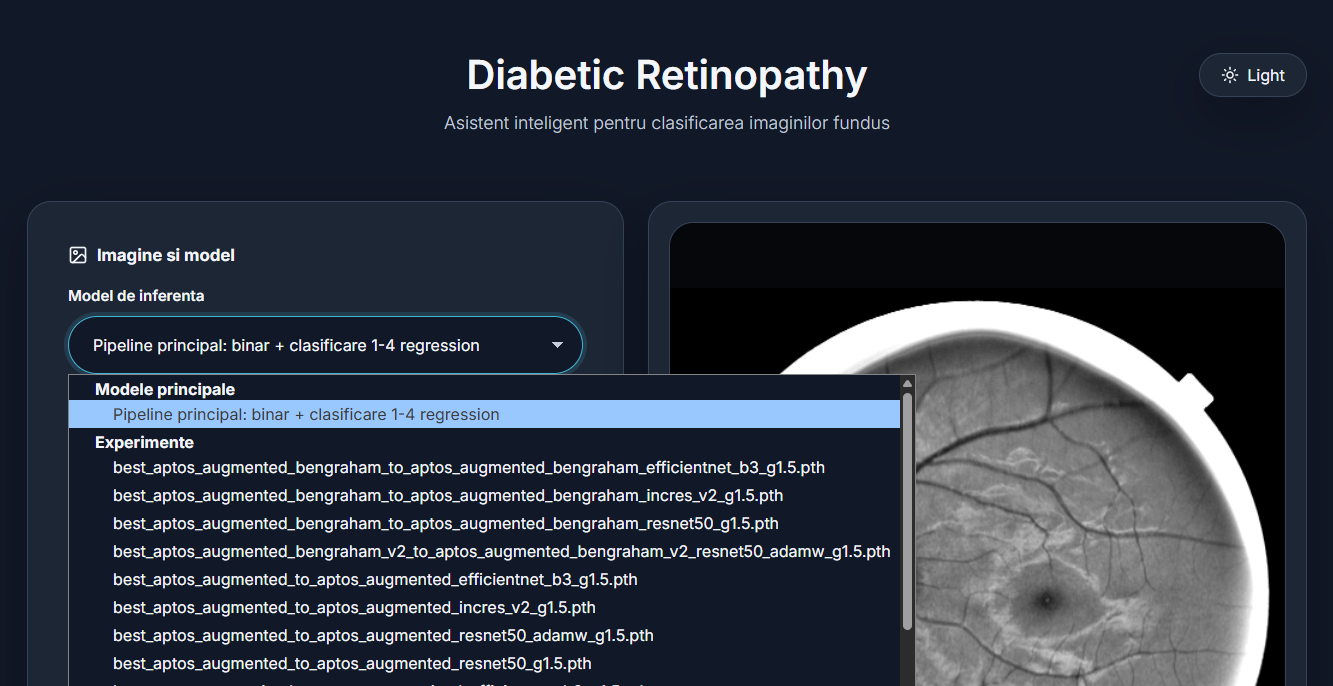
\includegraphics[width=0.95\textwidth]{Figuri/dropdown_menu_modele_website.png}
\captionsetup{justification=centering}
\caption{Meniul dropdown pentru selecția pipeline-ului principal și a modelelor experimentale}
\label{fig:dropdown-models}
\end{figure}

\section{Integrarea modelului antrenat}

\ \ \ \ Integrarea modelului antrenat diferă pentru cele două categorii din catalog. Pentru modelele
experimentale, backend-ul reutilizează funcția \texttt{get\_model} folosită în etapa de antrenare.
Fișierul \texttt{.pth} salvează ponderile, nu întreaga logică a arhitecturii, deci modelul trebuie
reconstruit înainte de încărcarea parametrilor. Backend-ul identifică arhitectura prin funcția
\texttt{get\_base\_model\_name}, analizând numele fișierului selectat.
\bigskip

Pentru pipeline-ul principal, arhitectura este reconstruită explicit în backend. Detectorul binar este
un \texttt{EfficientNet-B3} cu un singur neuron de ieșire și funcție sigmoid, iar clasificatorul de
severitate este un \texttt{EfficientNet-B3} cu ieșire scalară pentru regresie. Ponderile sunt încărcate
cu \texttt{torch.load}, folosind \texttt{map\_location} pentru compatibilitate cu dispozitivul disponibil.
Detectorul binar este încărcat din directorul \path{Rezultate_main/binar}, iar etapa de severitate din
\path{Rezultate_main/clasificare_regression}.
Pentru ramura de regresie, scorul continuu este transformat în clase prin \texttt{numpy.digitize} și
pragurile salvate în \texttt{rounder\_coef.npy}. În acest fel, aplicația poate rula atât scenariul final
al lucrării, cât și modelele multiclasă experimentale.

\section{Limitări practice ale aplicației}

\ \ \ \ Aplicația are rol demonstrativ și prezintă mai multe limitări. În primul rând,
verificarea preprocesării nu este echivalentă cu validarea medicală a imaginii și nu
garantează că imaginea are o calitate suficientă pentru diagnostic. În al doilea
rând, modelele sunt încărcate la fiecare cerere, ceea ce este simplu pentru
testare, dar ineficient pentru producție. În cazul pipeline-ului principal, încărcarea poate implica
două modele pentru a obține atât decizia binară, cât și informațiile despre severitate. Controlul calității imaginilor este o etapă importantă
în evaluarea sistemelor pentru retinopatie diabetică, deoarece imaginile neclare, slab iluminate sau
incorect centrate pot afecta predicția modelului \cite{14_liu2022deepdrid}.
\bigskip

Recomandările afișate sunt statice și orientative. Ele nu țin cont de istoricul
pacientului, de acuitatea vizuală, de edemul macular, de tratamente existente sau de
alte informații clinice. În plus, pragul operațional al detectorului binar din aplicație este o alegere
tehnică pentru prototip și ar trebui calibrat riguros înainte de orice utilizare clinică. Într-o
versiune reală, aplicația ar trebui să includă validare medicală, control al calității imaginilor,
autentificare, audit, stocare securizată și un mecanism de marcare a predicțiilor incerte. Integrarea
într-un flux clinic ar trebui însoțită și de explicabilitate și analiză a erorilor, astfel încât
deciziile modelului să poată fi interpretate de utilizatori umani \cite{9_chetoui2020explainable}.


\chapter{Concluzii și direcții viitoare}

\section{Concluzii generale}

\ \ \ \ Lucrarea a prezentat un sistem complet pentru clasificarea automată a retinopatiei diabetice
pe baza imaginilor de fund de ochi. Au fost analizate fundamentele medicale ale bolii,
stadiile de severitate, particularitățile imaginilor retiniene și direcțiile relevante din
literatura de specialitate. Pe această bază a fost construit un pipeline experimental în
PyTorch, folosind transfer learning, preprocesare dedicată imaginilor fundus și antrenare locală
pe CUDA.
\bigskip

Metodologia include două componente complementare. Prima componentă este reprezentată de
experimentele preliminare, prin care au fost comparate arhitecturi, funcții de pierdere,
optimizatori și variante de augmentare. A doua componentă este sistemul propus, organizat în
două etape: detecția binară a bolii și clasificarea severității pentru cazurile patologice. În
plus, a fost realizată o aplicație web de inferență, care demonstrează modul în care modelele
salvate pot fi utilizate într-o interfață practică.

\section{Rezultatele obținute față de obiectivele inițiale}

\ \ \ \ Obiectivele inițiale au fost îndeplinite în mai multe direcții. A fost realizată o analiză
a metodelor existente pentru detecția și clasificarea retinopatiei diabetice, au fost studiate
mai multe seturi de date publice, iar imaginile au fost reorganizate prin scripturi dedicate
pentru split, curățare, augmentare și preprocesare. De asemenea, a fost implementată o metodă
bazată pe rețele convoluționale și transfer learning, adaptată într-un sistem în două etape.
\bigskip

Codul permite testarea mai multor arhitecturi, funcții de pierdere și optimizatori. Au fost
generate modele salvate, grafice de evaluare și rapoarte de clasificare. O contribuție
importantă a lucrării este identificarea riscului de \textit{data leakage} în utilizarea
dataset-ului \newline \texttt{Diabetic\_Balanced\_Data} și construirea unui split grupat care păstrează
imaginea originală și augmentările ei în același subset. În plus, aplicația de inferență arată
că rezultatele experimentale pot fi integrate într-un flux software accesibil, în care
utilizatorul încarcă o imagine și primește o predicție.

\section{Limitările lucrării}

\ \ \ \ Principala limitare a sistemului propus este legată de propagarea erorilor în pipeline-ul în
două etape. Prima etapă decide dacă imaginea este sănătoasă sau patologică, iar această decizie
influențează direct interpretarea rezultatului final. Un fals negativ în etapa binară este critic,
deoarece o imagine cu retinopatie diabetică poate fi oprită înainte de gradarea severității și poate fi
raportată ca fiind fără boală. În sens invers, un fals pozitiv trimite o imagine sănătoasă către etapa
de clasificare 1--4, unde aceasta poate primi un grad scăzut de boală. Acest compromis este acceptabil
într-un context experimental orientat spre screening, deoarece reducerea fals-negativelor este prioritară,
dar ar necesita calibrare riguroasă și validare clinică înainte de utilizarea într-un scenariu real.
\bigskip 

O altă limitare importantă este faptul că modelele au fost evaluate pe seturi de date publice, care nu
reflectă complet variabilitatea clinică reală. În practică, imaginile pot proveni din camere diferite,
centre medicale diferite, populații diferite și protocoale diferite de achiziție, iar distribuția
claselor este de obicei dezechilibrată. Din acest motiv, performanța obținută pe un dataset public nu
garantează automat aceeași performanță într-un program real de screening. De asemenea, generalizarea
între dataset-uri rămâne dificilă, deoarece modelul poate învăța particularități ale sursei imaginilor,
nu doar semnele patologice ale retinopatiei diabetice.
\bigskip

O altă limitare este faptul că unele seturi publice conțin imagini augmentate sau foarte
asemănătoare între ele. În această lucrare, problema a fost investigată explicit pentru
\newline \texttt{Diabetic\_Balanced\_Data}, iar split-ul grupat reduce riscul ca originale și augmentări
să ajungă în subseturi diferite. Totuși, pentru o validare și mai strictă, ar fi utilă o
împărțire la nivel de pacient, astfel încât imagini apropiate provenite de la același pacient
să nu apară simultan în antrenare și testare.
\bigskip

Calitatea imaginilor reprezintă, la rândul ei, o limitare. Preprocesarea Ben Graham reduce variațiile
de iluminare și uniformizează parțial aspectul imaginilor, însă nu înlocuiește un modul clinic de
control al calității. Imaginile neclare, prost centrate, supraexpuse, subexpuse sau afectate de
artefacte pot influența predicția, mai ales în clasele apropiate vizual. Separarea dintre clasele 1, 2
și 3 rămâne dificilă, deoarece diferențele dintre stadii sunt uneori subtile chiar și pentru evaluarea
umană.
\bigskip 

Lucrarea nu include validare clinică realizată de medici oftalmologi și nu testează sistemul pe imagini
provenite strict din mai multe centre medicale. Prin urmare, aplicația de inferență are rol
demonstrativ și nu poate fi considerată un instrument medical. În forma actuală, aplicația este un
prototip tehnic, fără autentificare, audit, stocare securizată a datelor, integrare cu sisteme clinice
sau certificare medicală. În plus, explicațiile vizuale nu sunt integrate direct în fluxul aplicației,
ceea ce limitează interpretabilitatea fiecărei predicții pentru un utilizator medical.

\section{Direcții viitoare}

\ \ \ \ O primă direcție viitoare este calibrarea explicită a pragului detectorului binar și analiza
separată a fals-negativelor și fals-pozitivelor produse de pipeline-ul în două etape. Într-o versiune
mai avansată, pragul nu ar trebui ales doar ca valoare operațională fixă, ci optimizat în funcție de
scopul aplicației: sensibilitate ridicată pentru screening, specificitate mai mare pentru reducerea
alarmelor false sau un compromis stabilit împreună cu specialiști clinici. De asemenea, cazurile cu
probabilitate apropiată de prag ar putea fi marcate ca incerte și trimise automat către revizuire
umană.
\bigskip
 
O direcție de modelare ar fi înlocuirea etapei de clasificare 1--4 cu un model multiclasă 0--4,
dar păstrând detectorul binar ca filtru inițial. În această variantă, imaginile pentru care detectorul
binar indică foarte sigur clasa 0 ar putea fi eliminate din analiza suplimentară, iar restul imaginilor
ar fi trimise către un clasificator complet 0--4. Această soluție ar permite modelului de severitate să
învețe explicit și clasa sănătoasă, reducând riscul ca un fals pozitiv al detectorului binar să fie
forțat automat într-una dintre clasele 1--4. În același timp, filtrarea cazurilor sigur sănătoase ar
păstra avantajul sistemului în două etape, deoarece etapa multiclasă s-ar concentra mai ales pe
imaginile ambigue sau suspecte.
\bigskip

Pentru îmbunătățirea generalizării, modelele ar trebui antrenate și pe seturi externe de date, nu doar
validate pe acestea. Integrarea unor imagini provenite din surse diferite ar expune rețeaua la camere,
rezoluții, niveluri de iluminare și distribuții de clase mai variate. O astfel de strategie ar putea
reduce dependența de particularitățile unui singur dataset și ar apropia procesul de antrenare de
condițiile întâlnite într-un scenariu real.
\bigskip

O altă direcție este îmbunătățirea augmentărilor, astfel încât acestea să reproducă mai potrivit
diversitatea imaginilor fundus. Pe lângă transformările geometrice și cromatice uzuale, ar putea fi
introduse variații controlate de iluminare, contrast, claritate, câmp vizual, artefacte de achiziție și
diferențe între camere. Scopul nu ar fi doar creșterea artificială a numărului de imagini, ci simularea
unor condiții realiste care să ajute modelul să devină mai robust.
\bigskip

În aceeași direcție, poate fi explorată și generarea de imagini sintetice de fund de ochi pentru
diferite grade de retinopatie diabetică, folosind modele generative de imagini. Această abordare ar
putea fi utilă mai ales pentru clasele mai slab reprezentate, unde numărul de exemple reale este redus.
Totuși, imaginile sintetice ar trebui folosite cu prudență și validate din punct de vedere vizual și
medical, deoarece un generator poate introduce artefacte nerealiste sau leziuni care nu respectă
distribuția clinică reală. Prin urmare, datele sintetice ar trebui privite ca o completare a
dataset-urilor reale, nu ca un înlocuitor al acestora.
\bigskip

Pe partea de arhitecturi, pot fi explorate modele de ultimă generație, precum Vision Transformers
(ViT) sau variante hibride CNN-Transformer. Acestea pot surprinde relații globale între regiuni
îndepărtate ale imaginii, ceea ce poate fi util în analiza retinei, unde severitatea nu depinde
întotdeauna de o singură leziune locală, ci de distribuția mai multor semne patologice. Compararea lor
cu EfficientNet-B3, ResNet50 și Inception-ResNet-V2 ar permite evaluarea beneficiului real al acestor
arhitecturi în raport cu costul computațional mai ridicat.
\bigskip

În completare, sistemul poate fi extins cu un modul de control al calității imaginii și cu metode de
explicabilitate vizuală. Înainte de clasificare, aplicația ar putea verifica dacă fotografia este clară,
bine iluminată și centrată, iar cazurile neconforme ar putea fi respinse sau marcate pentru
recapturare. După predicție, integrarea unor hărți de activare sau a unei segmentări de leziuni ar face
rezultatul mai ușor de interpretat. Aplicația de inferență poate fi, de asemenea, îmbunătățită prin
păstrarea modelelor în memorie, definirea unor praguri de incertitudine și generarea unor rapoarte
exportabile.

\newpage
\mbox{}
\newpage

\appendix
\bibliographystyle{unsrt}
\bibliography{referinte}

\chapter {Cod}

% \lstinputlisting[language=python, caption={builder.py -- construirea modelelor, funcțiilor de pierdere și optimizatorilor}]{../Notebooks/Main/builder.py}
% \vspace{1cm}

% \lstinputlisting[language=python, caption=my\_dataset.py -- \^{i}nc\u0103rcarea setului de date echilibrat]{../Notebooks/Main/my_dataset.py}
% \vspace{1cm}

% \lstinputlisting[language=python, caption=train.py -- antrenarea, evaluarea \c{s}i generarea graficelor]{../Notebooks/Main/train.py}
% \vspace{1cm}

\end{document}

